\documentclass{beamer}
\usetheme{Boadilla}
\usepackage{hyperref}
\usepackage{graphicx}
\usepackage{subfig}
\usepackage[
    backend=biber, 
    natbib=true,
    style=numeric,
    sorting=none,
    style=verbose-ibid,
    labelyear
]{biblatex}
\addbibresource{citations.bib}

\title{Real-time HPSS}
\subtitle{Real-time median-filtering harmonic-percussive source separation}
\author{Sevag Hanssian}
\institute{McGill University}
\setbeamertemplate{navigation symbols}{}

\begin{document}

\begin{frame}
\maketitle
\end{frame}

\begin{frame}
	\frametitle{What and why}
	HPSS is harmonic-percussive source separation. Using HPSS one can decompose an audio signal consisting of pitched, harmonic sound + percussive sound into separated harmonic and percussive signals.\\\ \\
	Useful algorithms exist for
	\begin{enumerate}
		\item harmonic sound -- key detection, chord detection, pitch detection, etc.
		\item percussive sound -- tempo estimation, beat tracking, onset detection, etc.
	\end{enumerate}
	Given mixed harmonic-percussive audio, apply HPSS as a pre-processing step to improve results.\footfullcite{whyhpss} Applying HPSS in real-time enables the same use as a pre-processing step for real-time algorithms/systems.
\end{frame}

\begin{frame}
	\frametitle{Harmonic sound}
	Harmonic sounds exhibit spectral sparseness (narrowband sounds) and temporal smoothness (steady sounds) i.e. horizontal lines\footfullcite{spectraldesc}\\
	\begin{figure}
	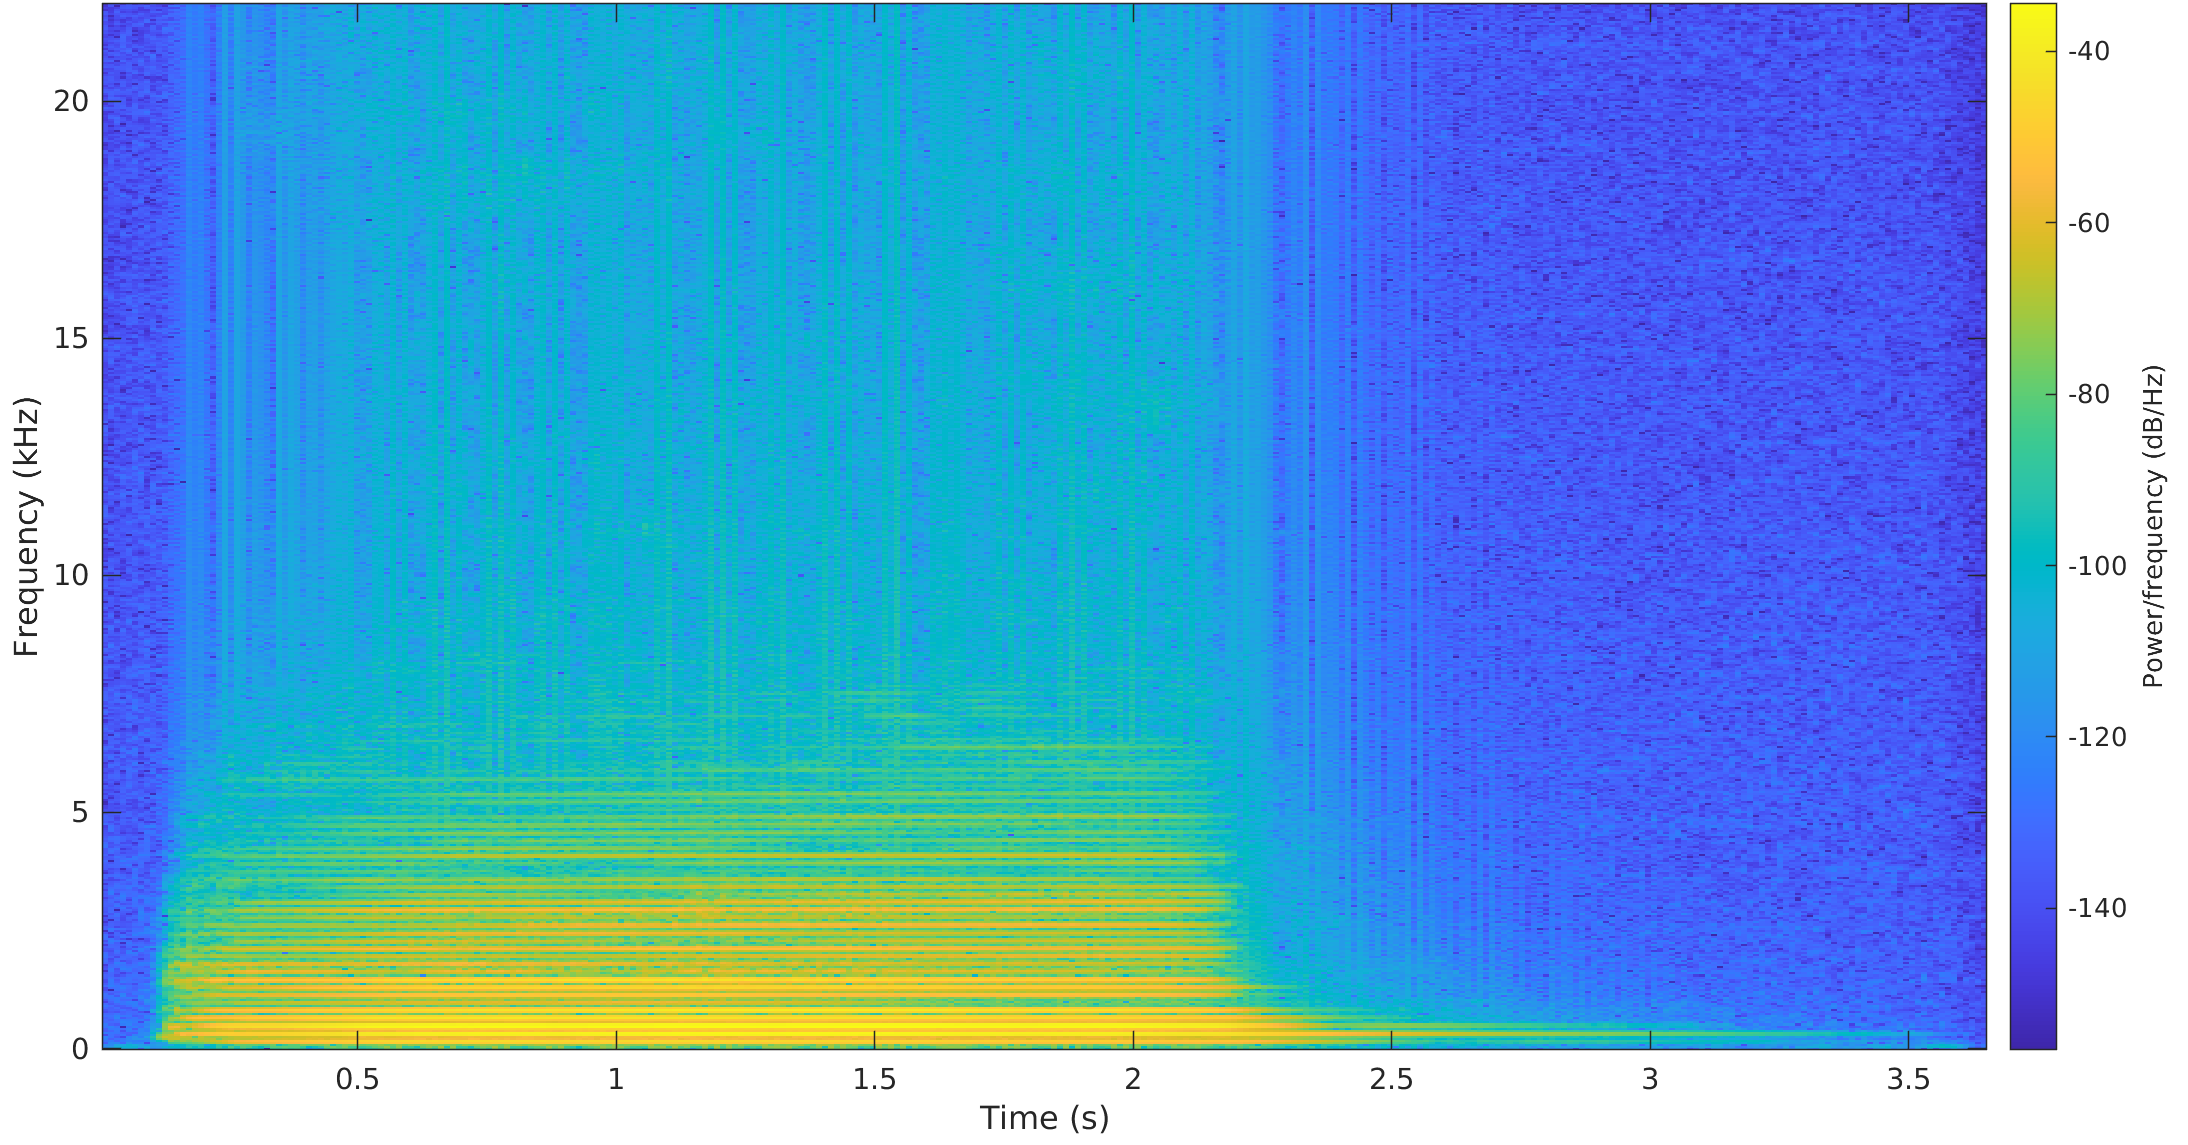
\includegraphics[height=5cm]{../images/violaspecgram.png}
		\caption{Harmonic spectrogram}
	\end{figure}
\end{frame}

\begin{frame}
	\frametitle{Harmonic sound}
	\href{run:../audio/viola.wav}{Click to listen}\\
	\begin{figure}
	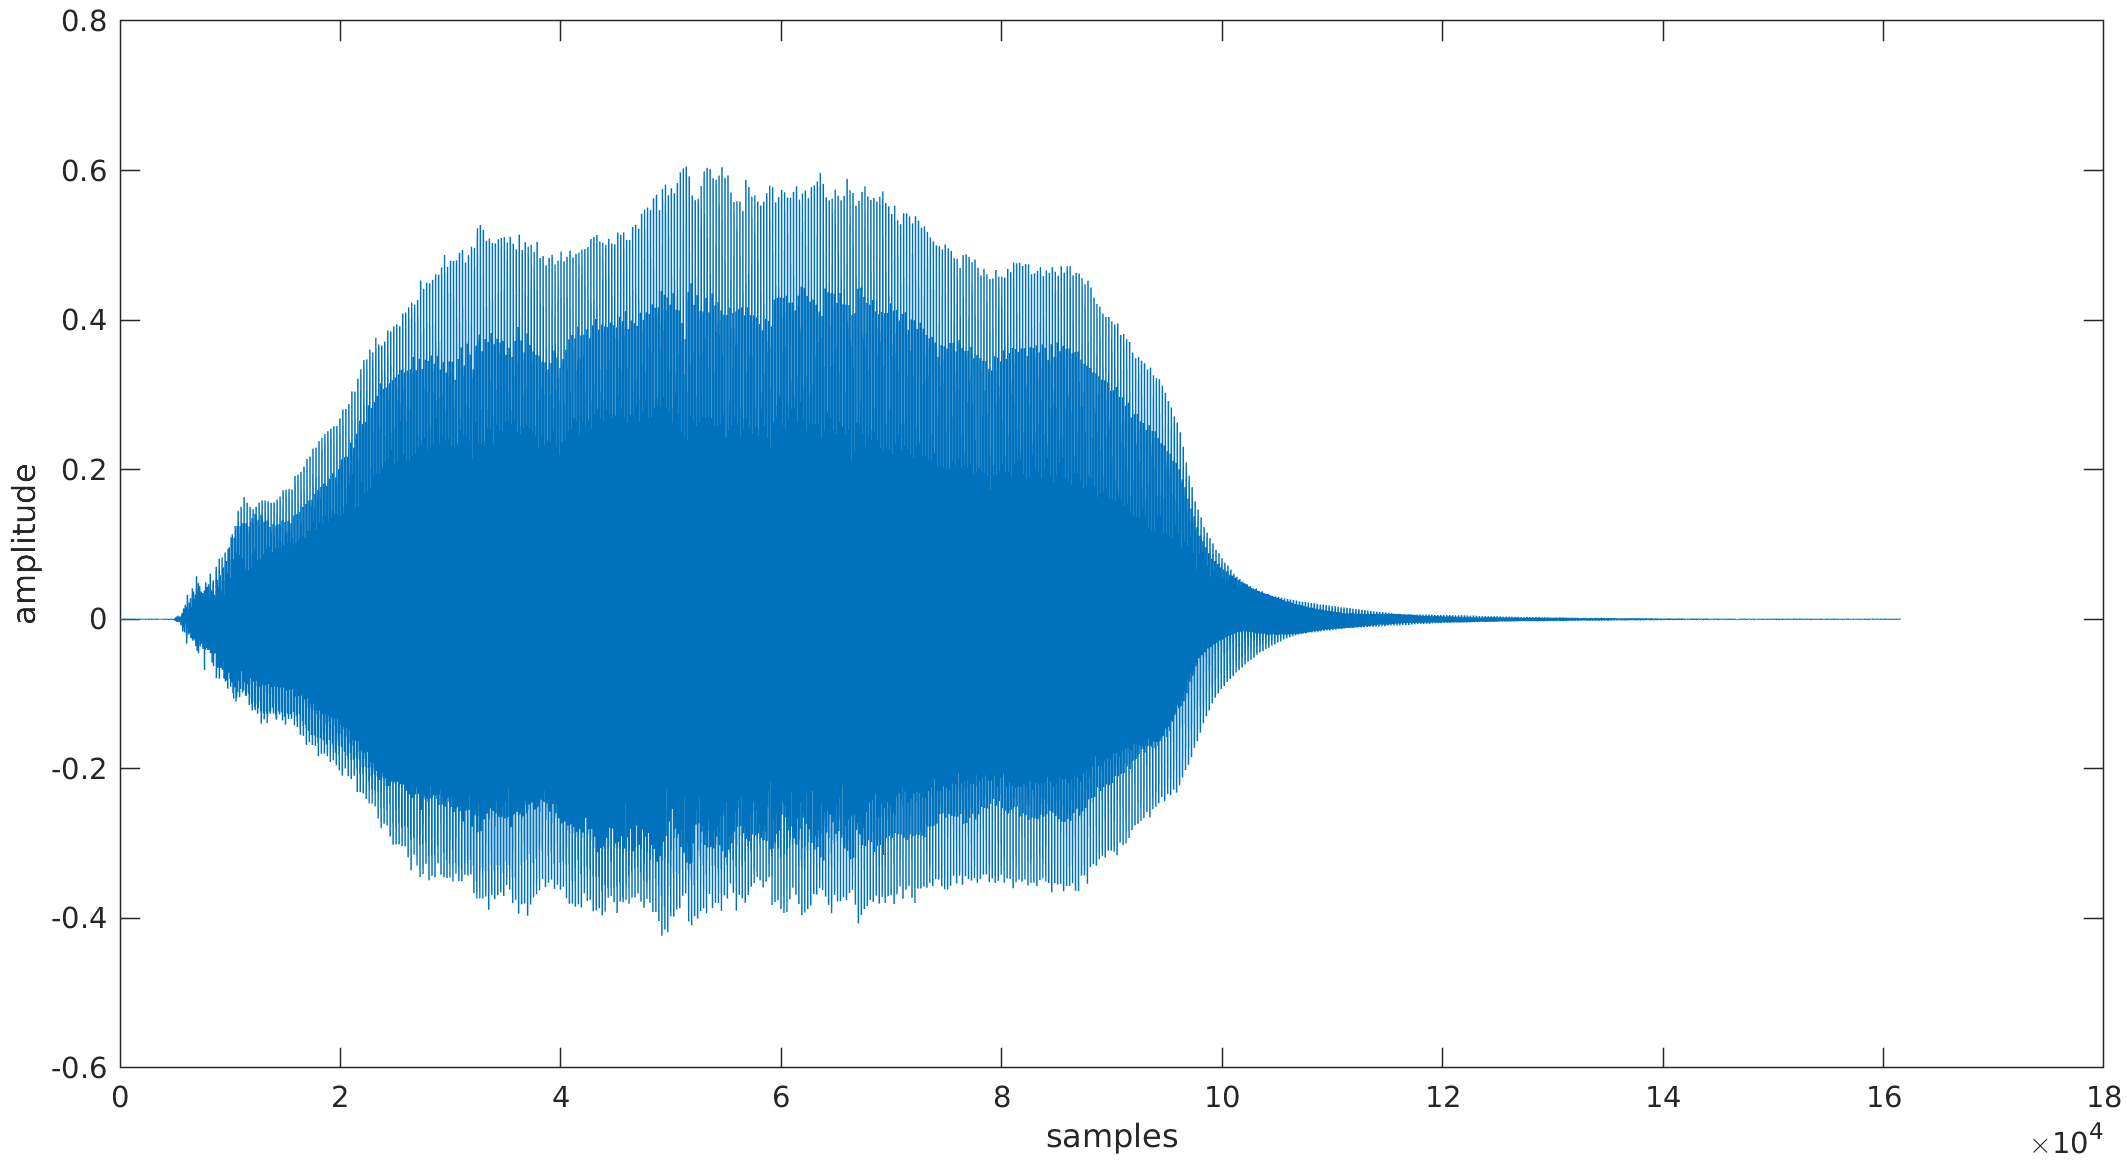
\includegraphics[width=10cm]{../images/viola_waveform.png}
		\caption{Harmonic time-domain waveform}
	\end{figure}
\end{frame}

\begin{frame}
	\frametitle{Percussive sound}
	Percussive sounds exhibit spectral smoothness (broadband sounds) and temporal sparseness (transient sounds) i.e. vertical lines\footfullcite{spectraldesc}\\
	\begin{figure}
	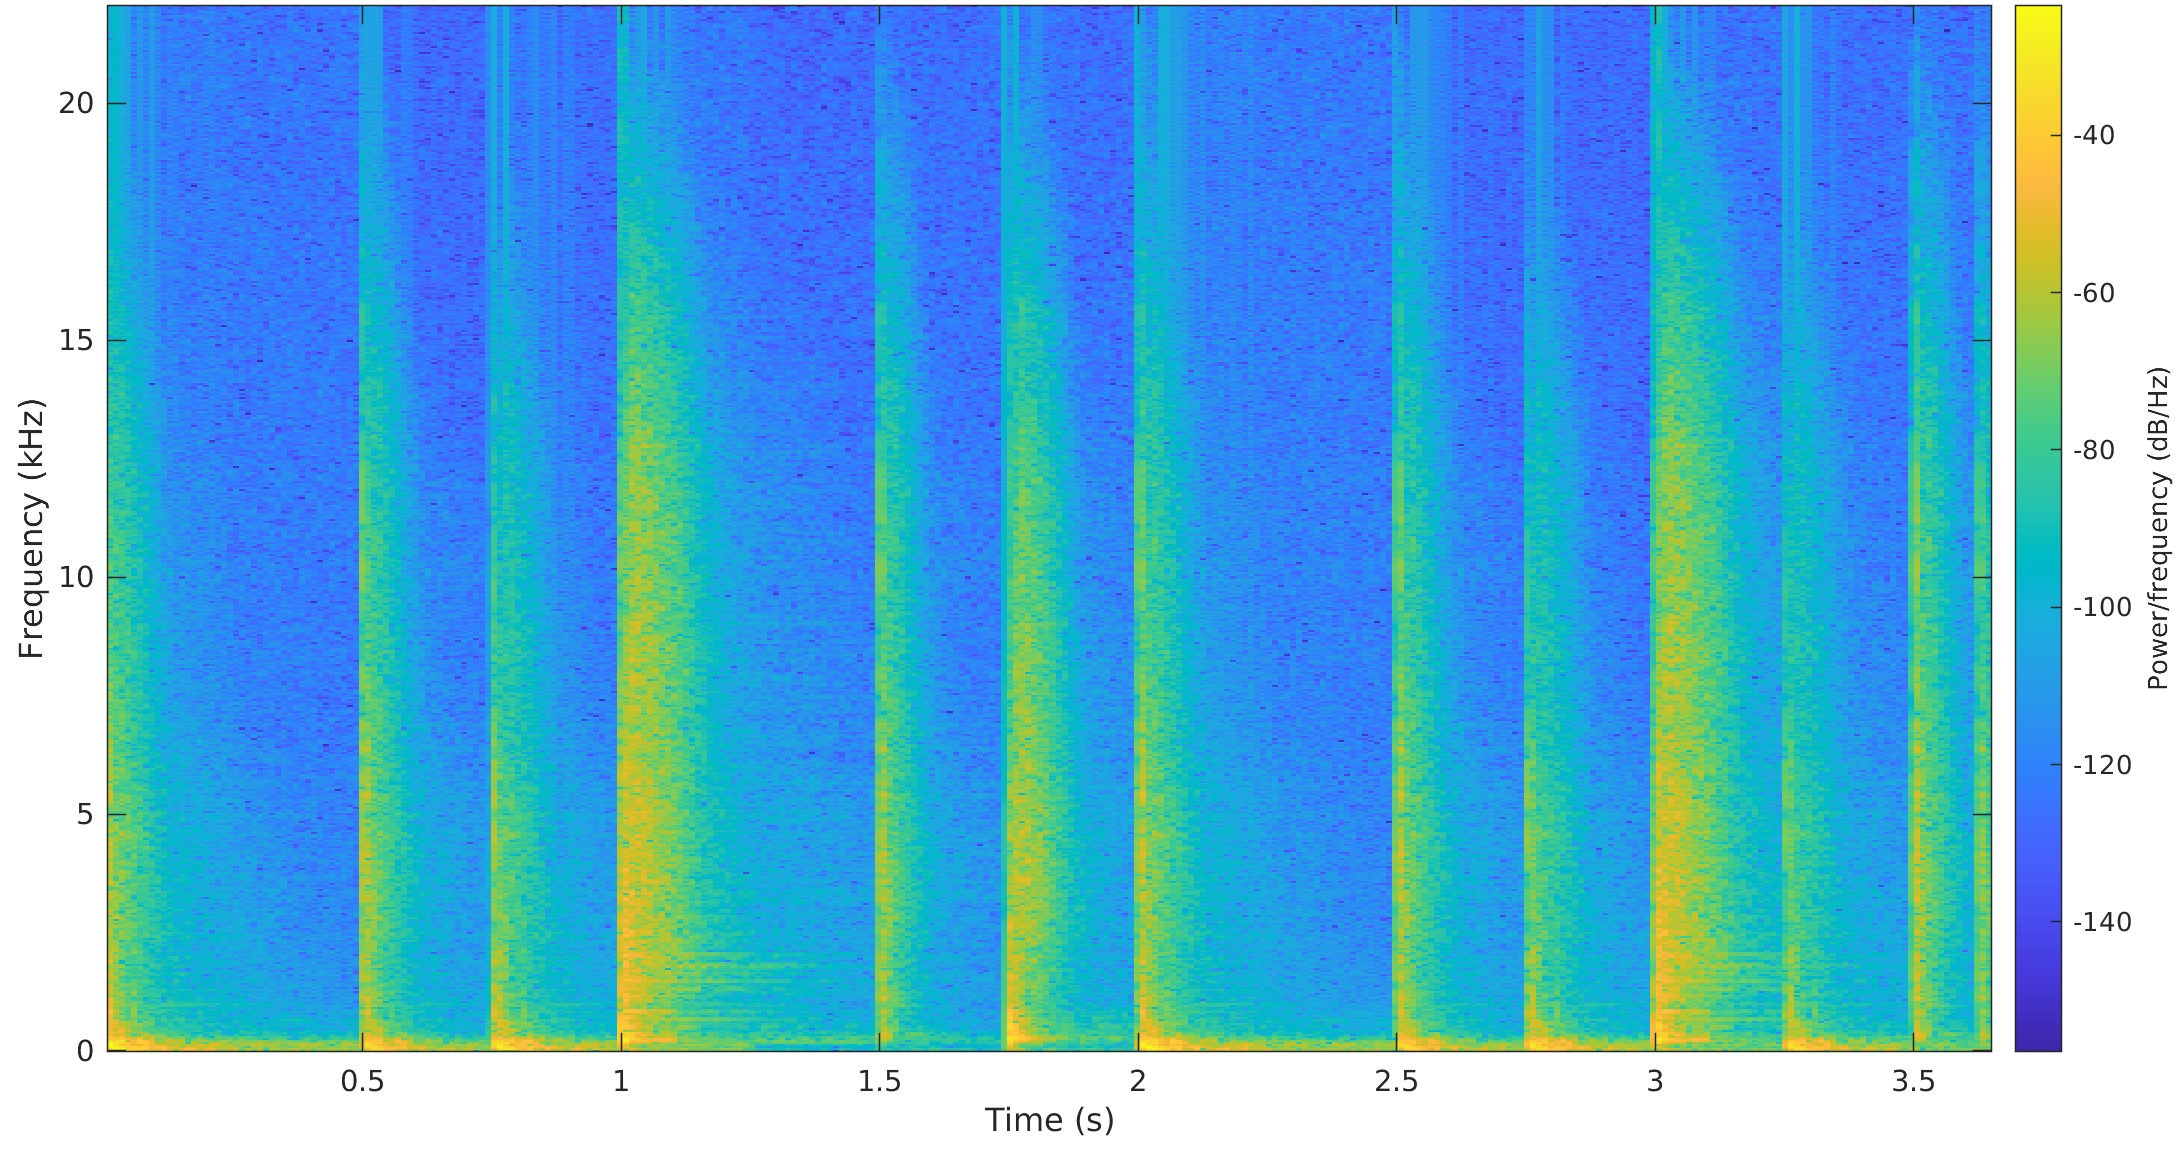
\includegraphics[height=5cm]{../images/drumspecgram.png}
		\caption{Percussive spectrogram}
	\end{figure}
\end{frame}

\begin{frame}
	\frametitle{Percussive sound}
	\href{run:../audio/drum.wav}{Click to listen}\\
	\begin{figure}
	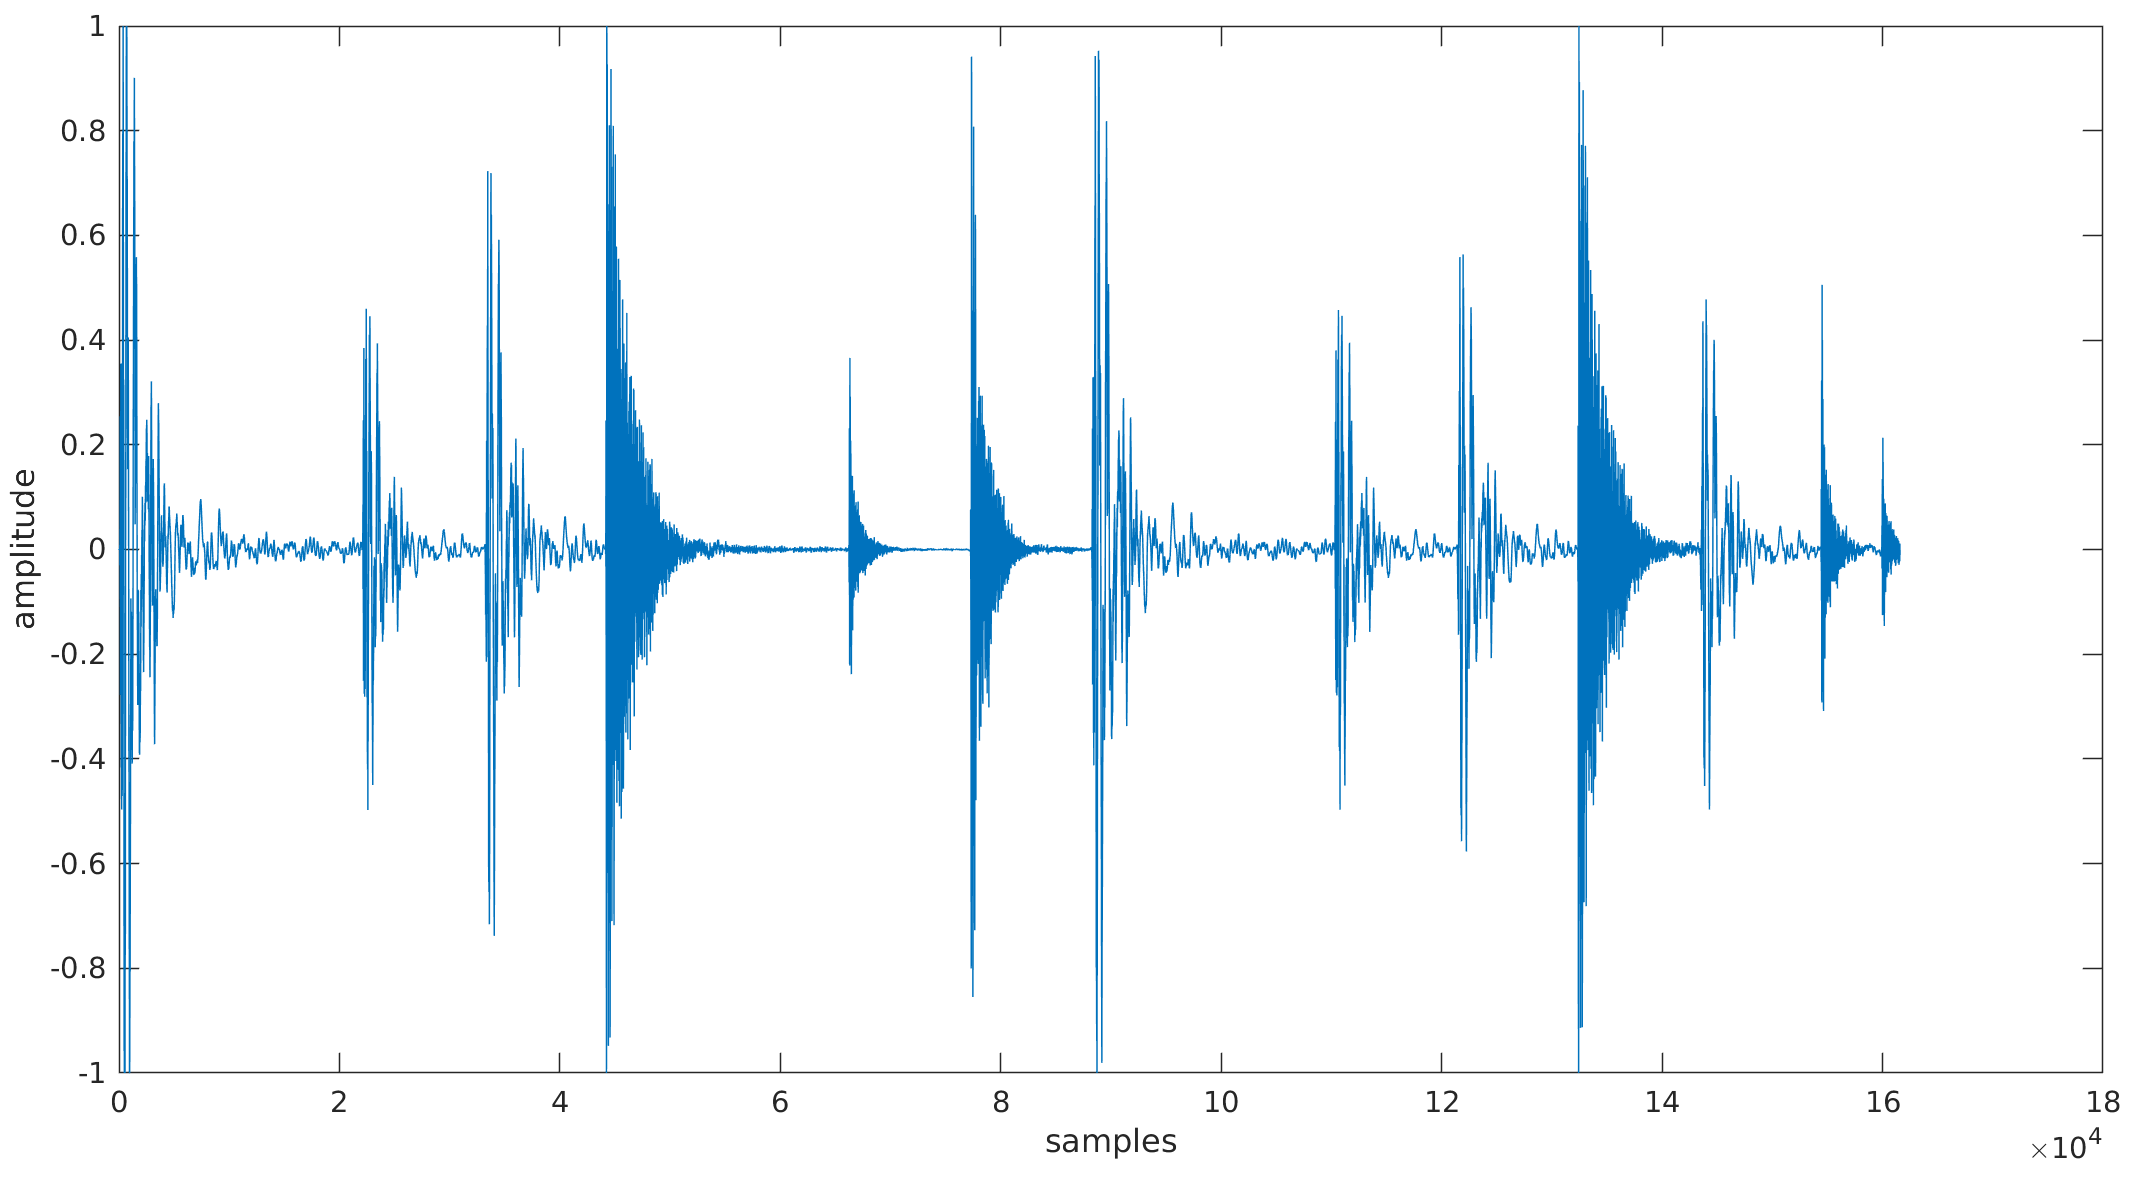
\includegraphics[height=5cm]{../images/drum_waveform.png}
		\caption{Percussive time-domain waveform}
	\end{figure}
\end{frame}

\begin{frame}
	\frametitle{Mixed sound}
	Combination of harmonic sound (horizontal lines) and percussive sound (vertical lines)\\
	\begin{figure}
	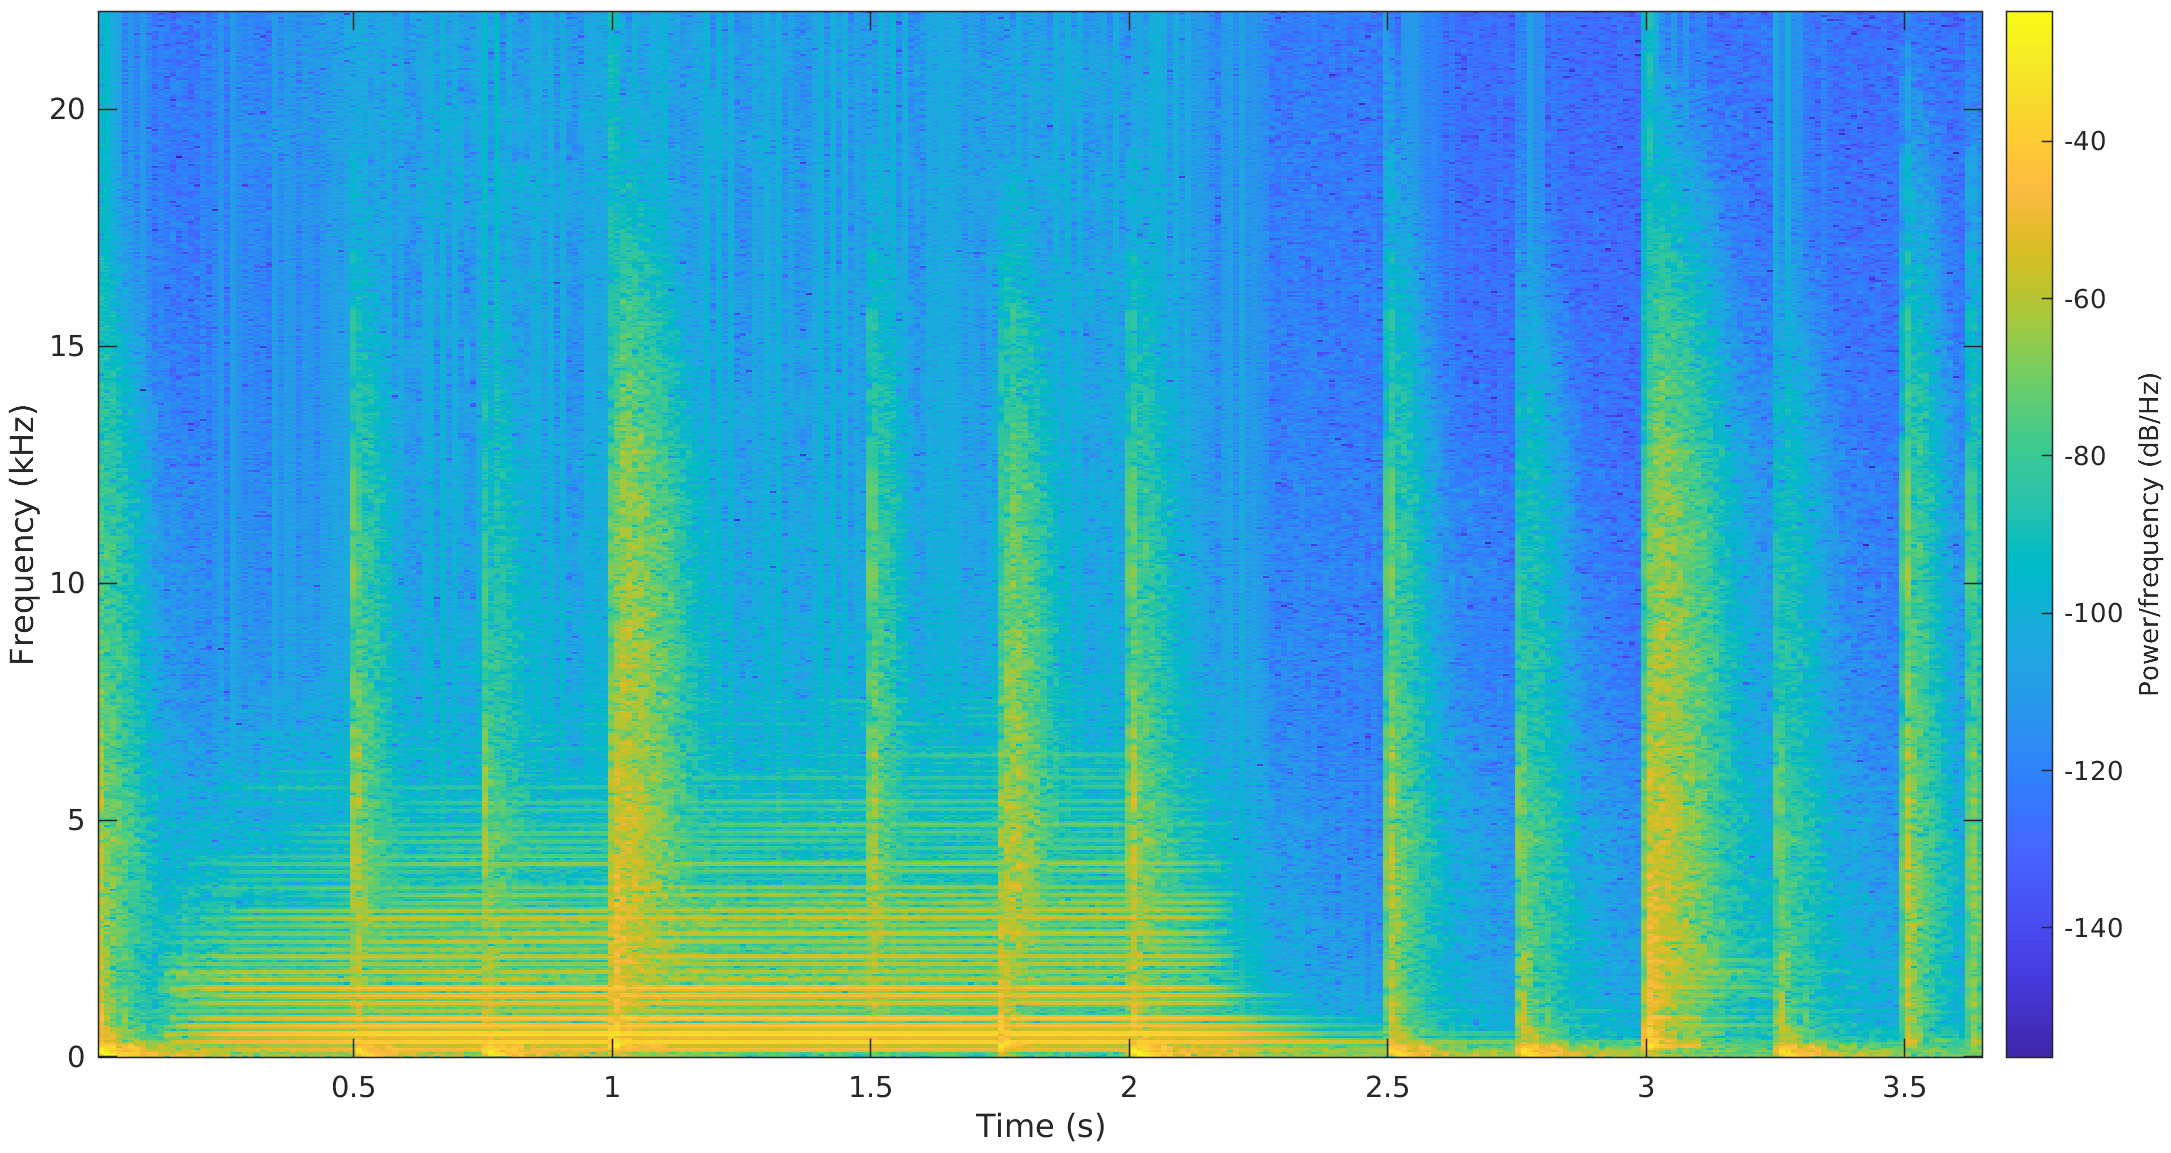
\includegraphics[height=5cm]{../images/mixedspecgram.png}
		\caption{Mixed spectrogram}
	\end{figure}
\end{frame}

\begin{frame}
	\frametitle{Mixed sound}
	\href{run:../audio/mixed.wav}{Click to listen}\\
	\begin{figure}
	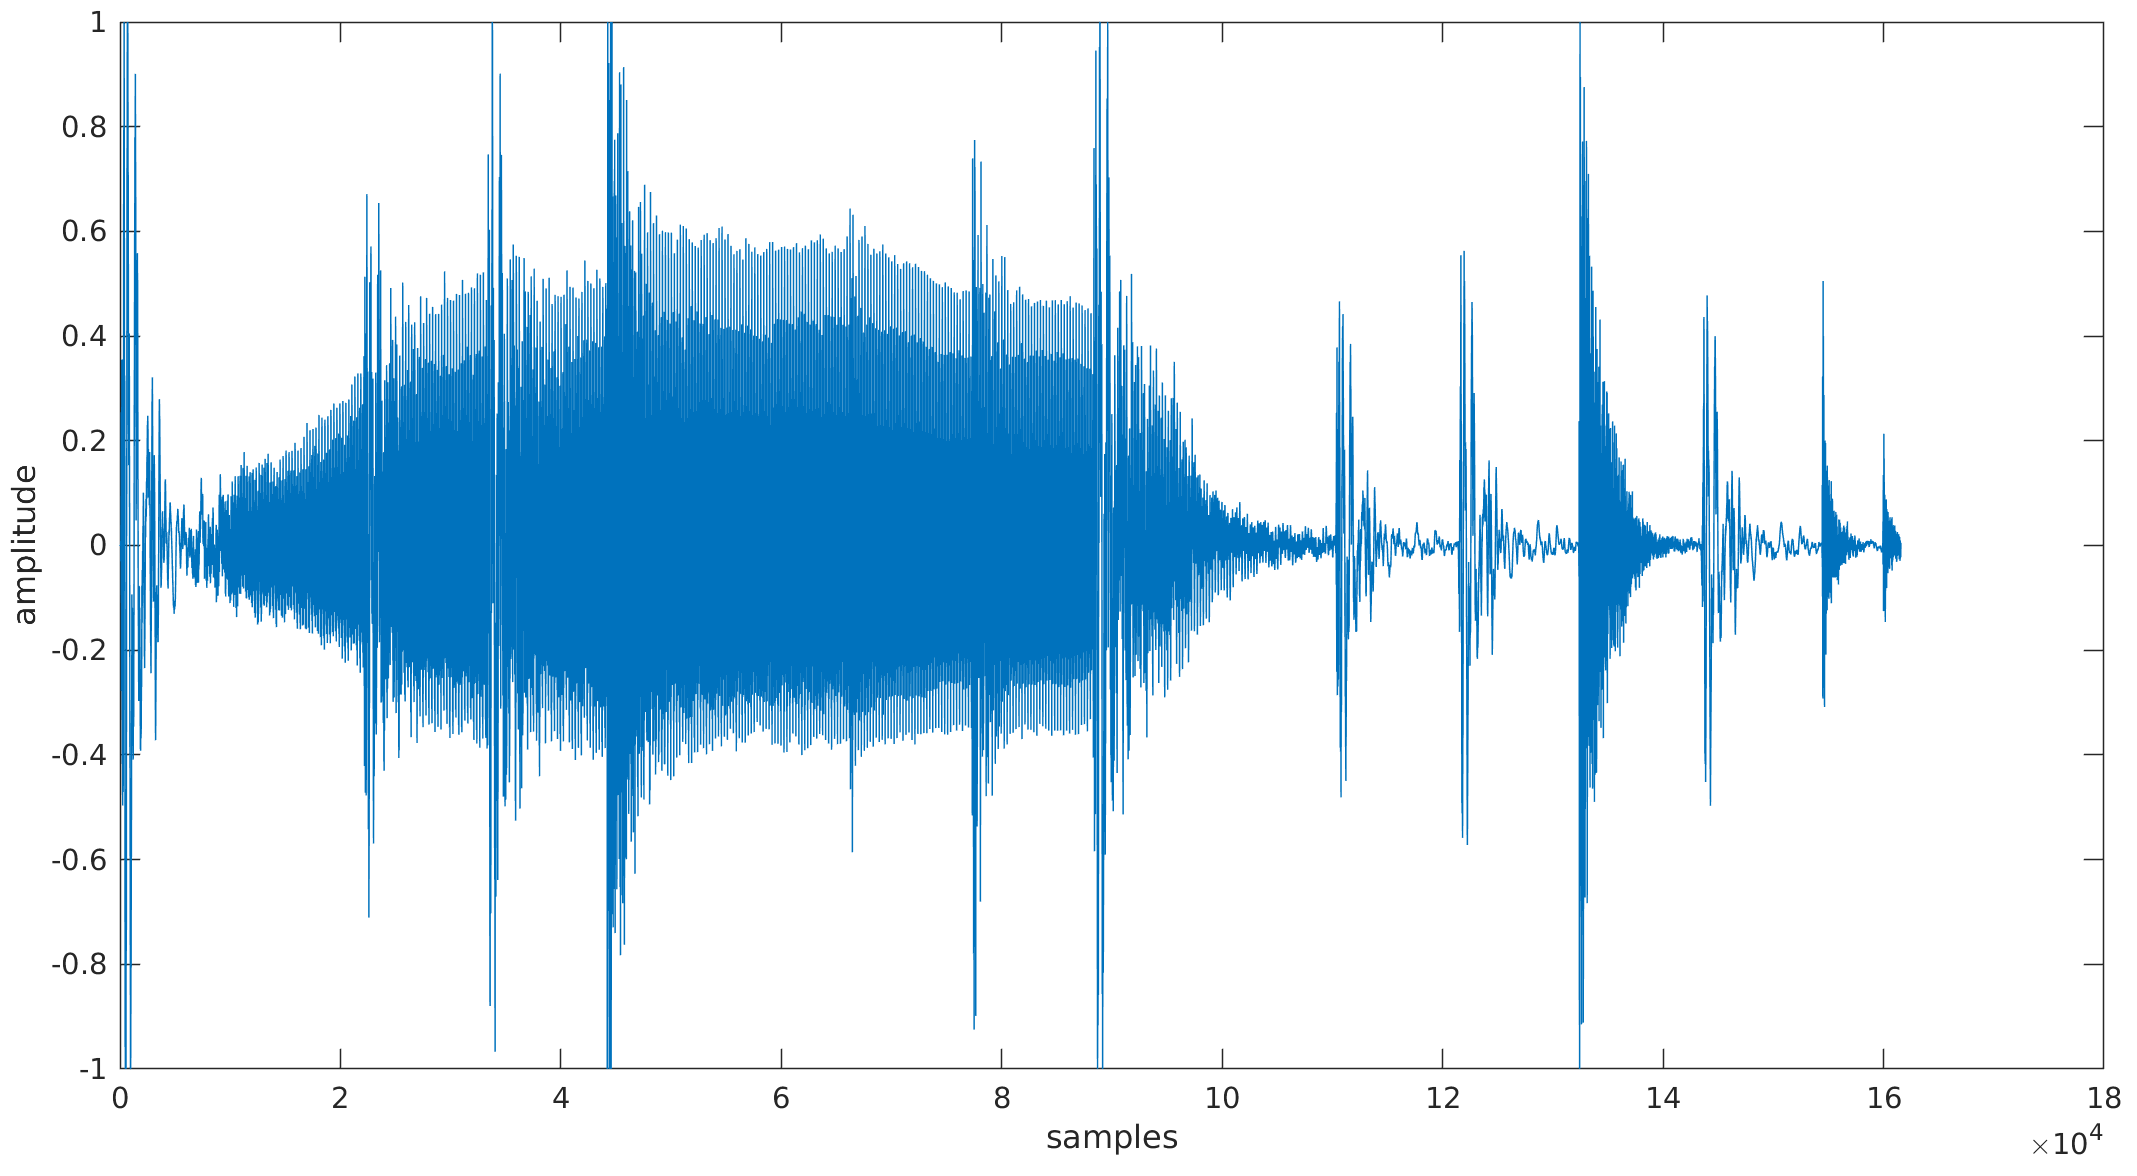
\includegraphics[height=5cm]{../images/mixed_waveform.png}
		\caption{Mixed time-domain waveform}
	\end{figure}
\end{frame}

\begin{frame}
	\frametitle{Median filtering images}
	Separate vertical and horizontal lines in the image domain with median filtering. Used in image denoising.\footfullcite{imagenoise}
	\begin{figure}
	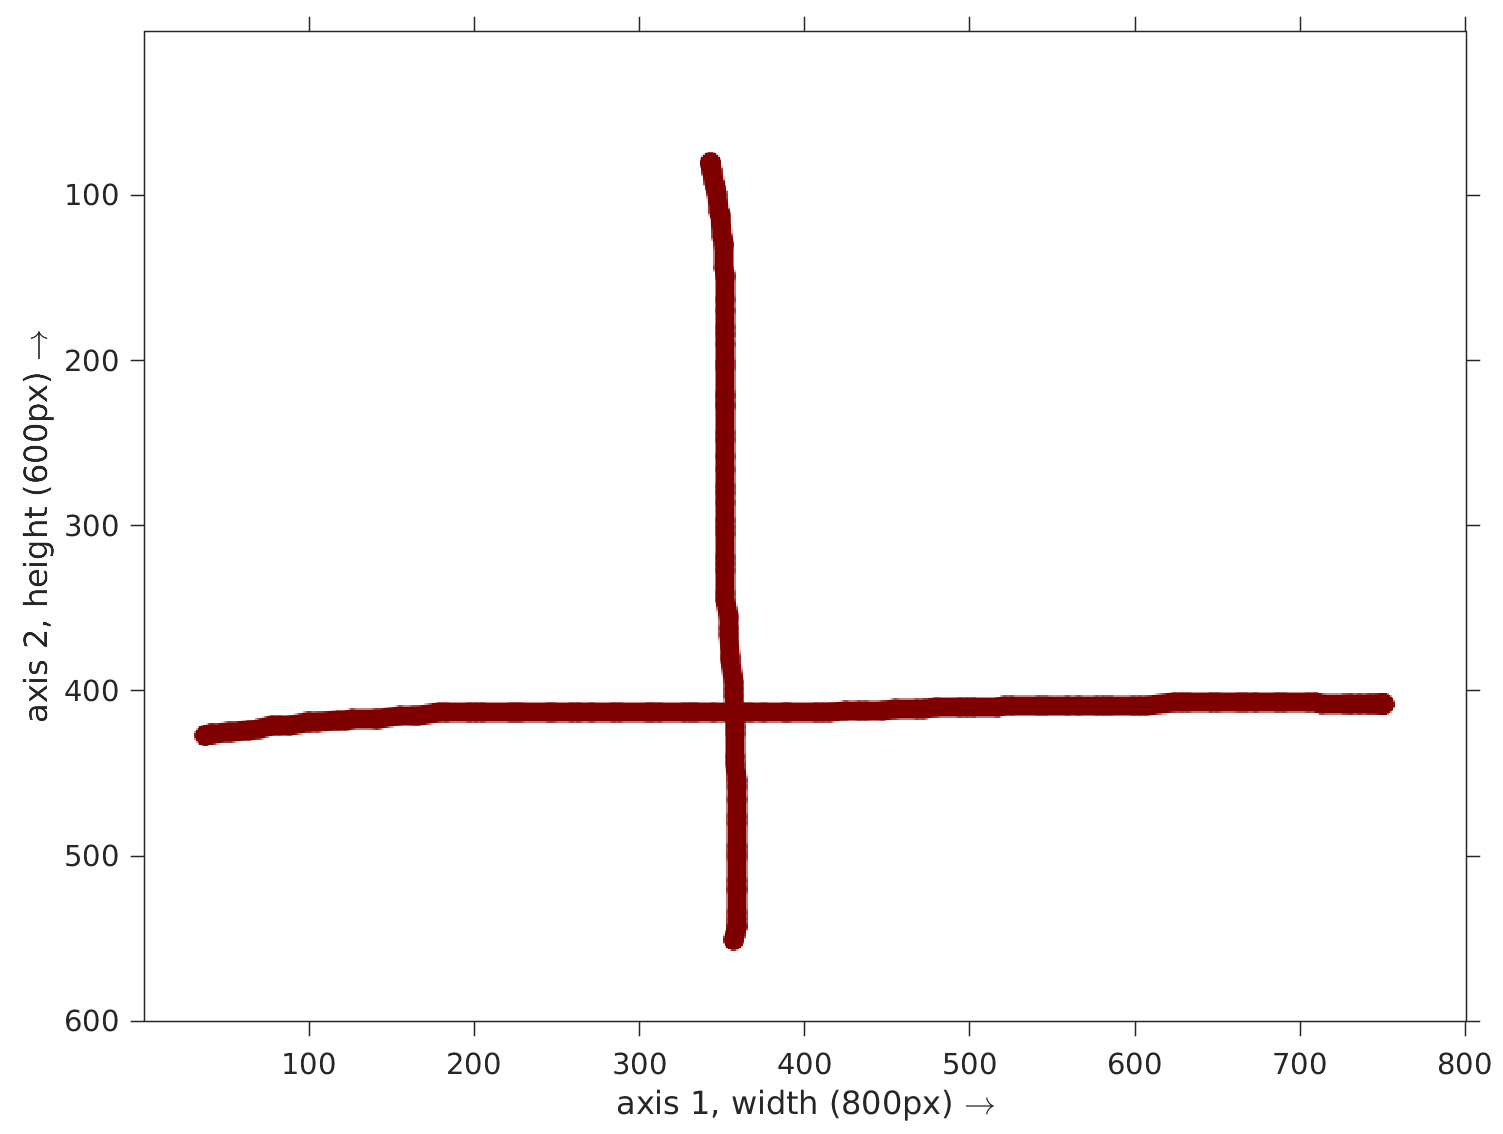
\includegraphics[width=6cm]{../images/medfilter_basic_with_axes.png}
		\caption{Mixed lines}
	\end{figure}
\end{frame}

\begin{frame}
	\frametitle{Median filtering images}
	movmedian(img, k, 1) = k-element sliding median for each column\\
	Emphasize vertical lines
	\begin{figure}
	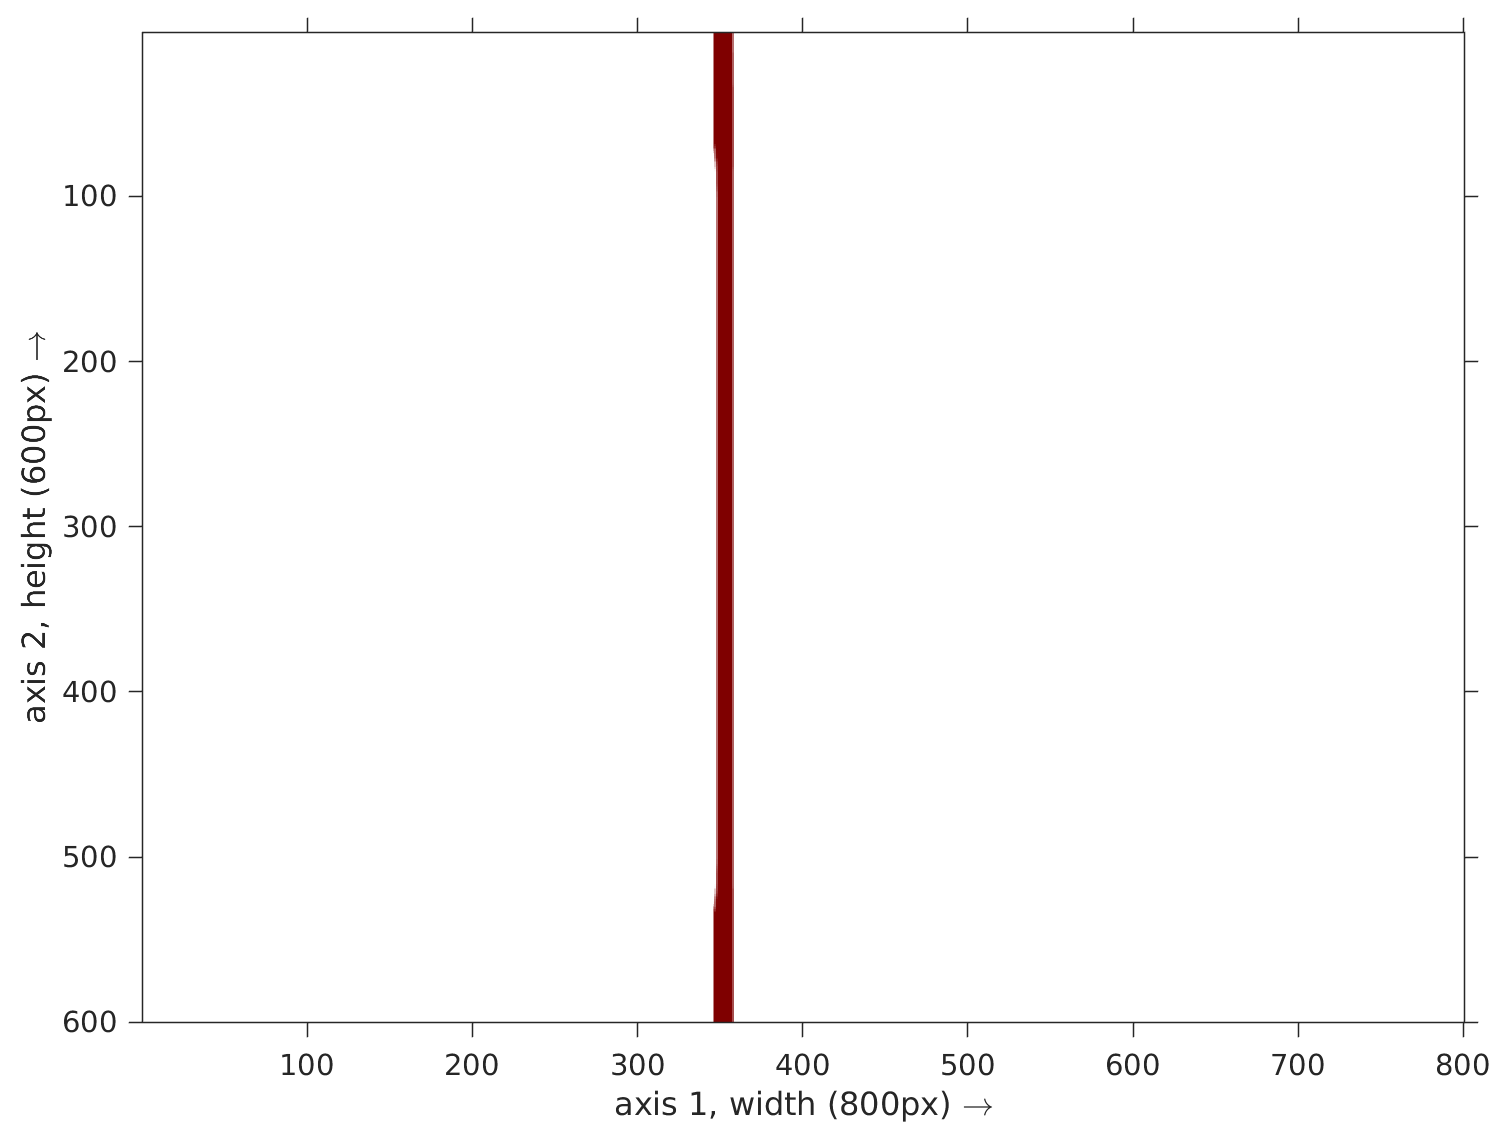
\includegraphics[width=6cm]{../images/medfilter_basic_axis1.png}
		\caption{vertical median filter}
	\end{figure}
\end{frame}

\begin{frame}
	\frametitle{Median filtering images}
	movmedian(img, k, 2) = k-element sliding median for each row\\
	Emphasize horizontal lines
	\begin{figure}
	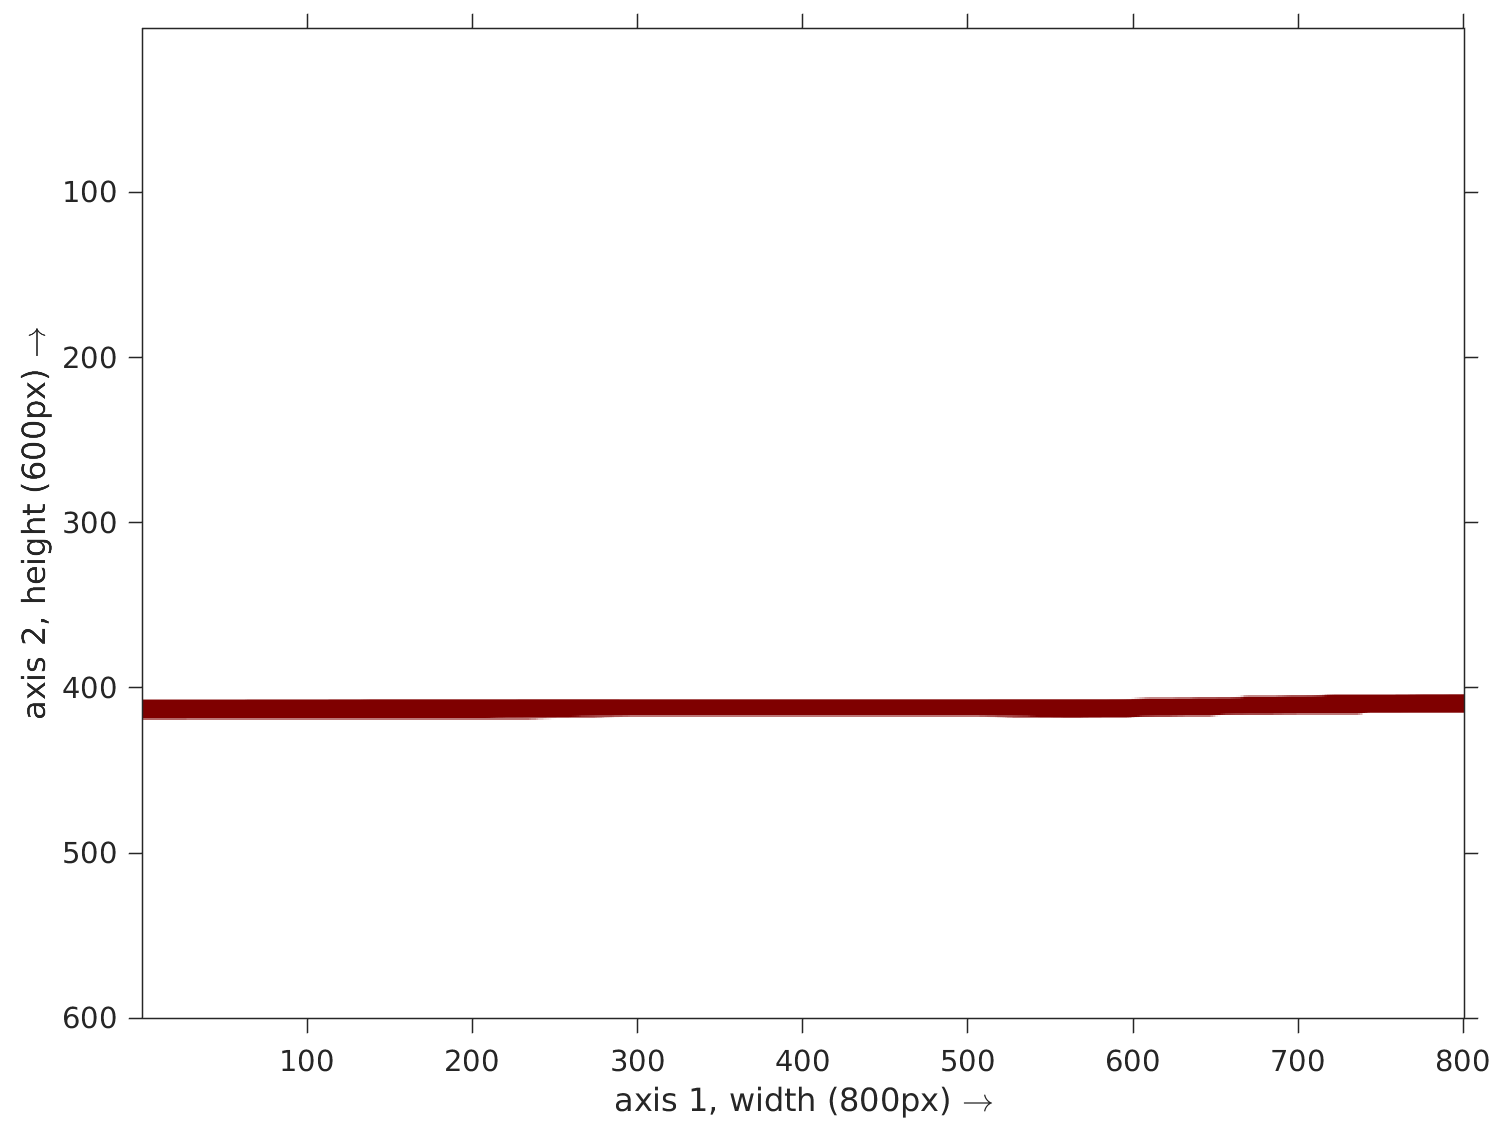
\includegraphics[width=6cm]{../images/medfilter_basic_axis2.png}
		\caption{horizontal median filter}
	\end{figure}
\end{frame}

\begin{frame}
	\frametitle{Median filtering spectrograms}
	Separate horizontal and vertical lines in the spectrogram
	\begin{figure}
	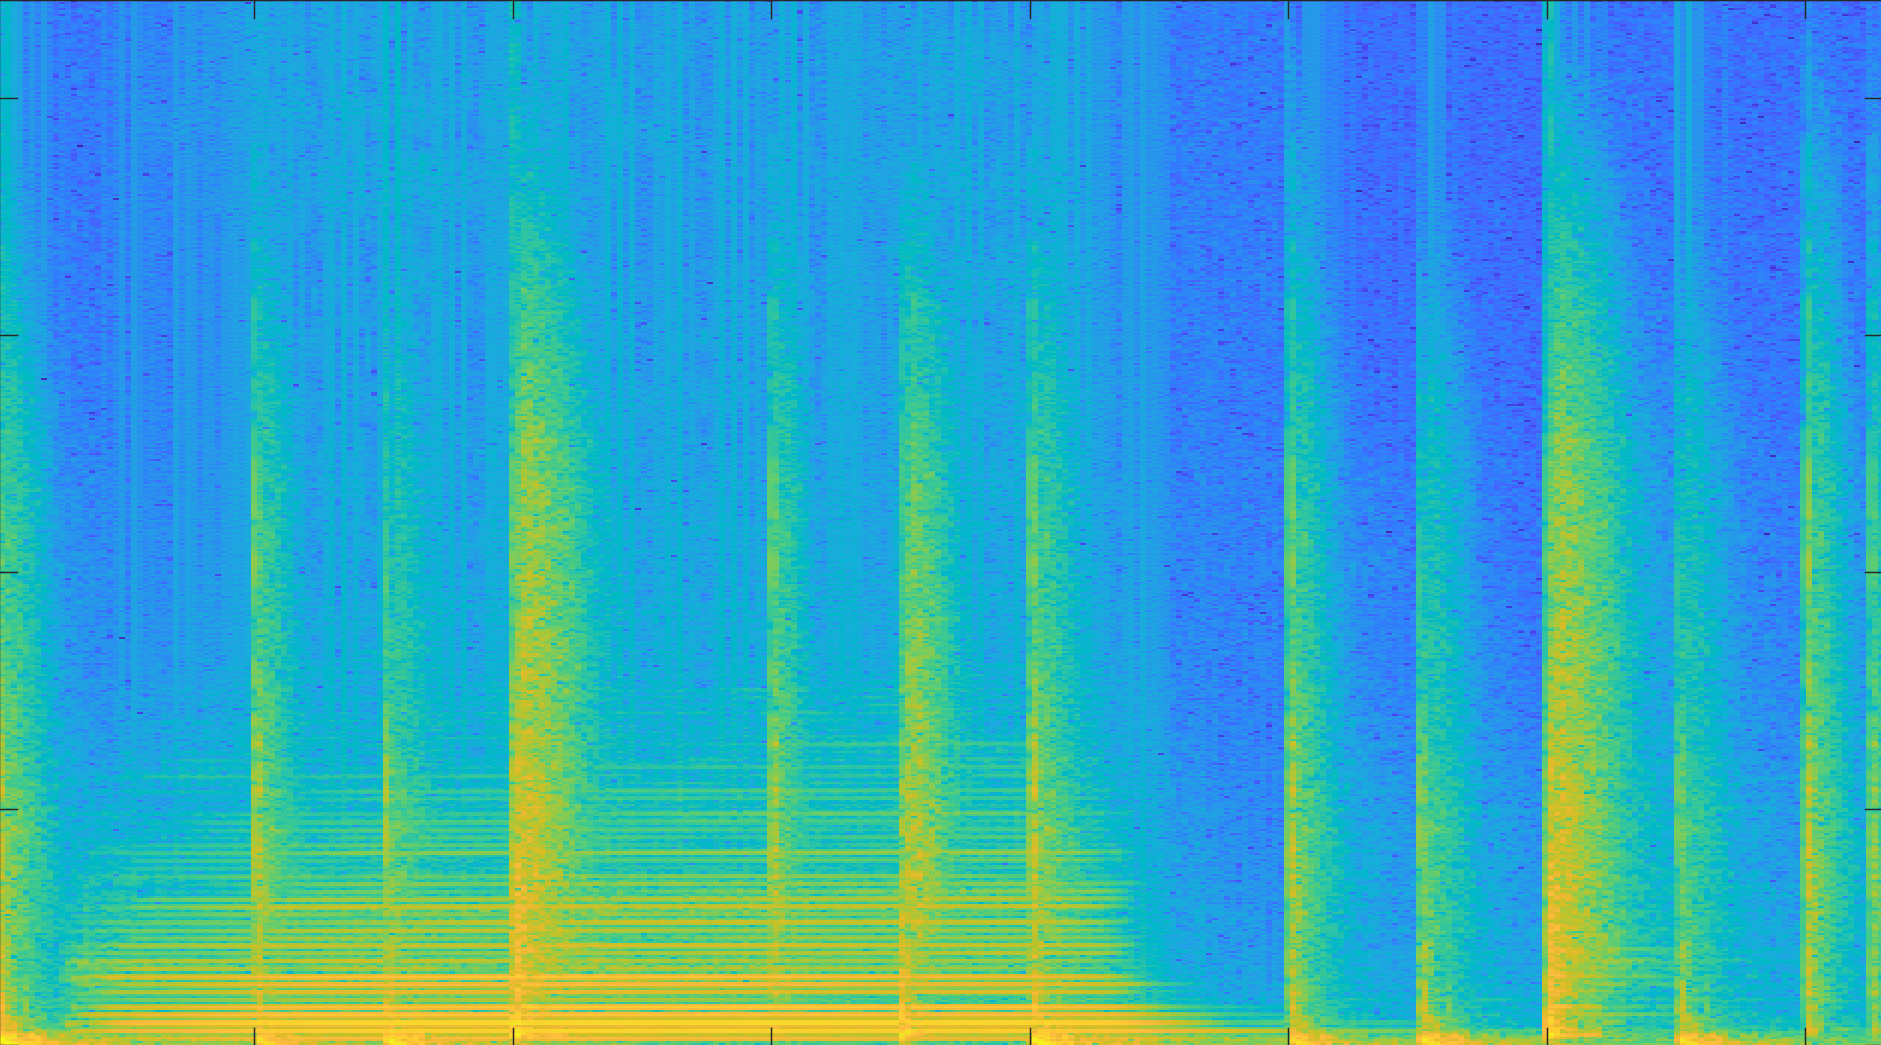
\includegraphics[height=5cm]{../images/mixedspecgram_cropped.png}
		\caption{Mixed spectrogram}
	\end{figure}
\end{frame}

\begin{frame}
	\frametitle{Median filtering spectrograms}
	Vertical median filter = ``percussive separation''
	\begin{figure}
	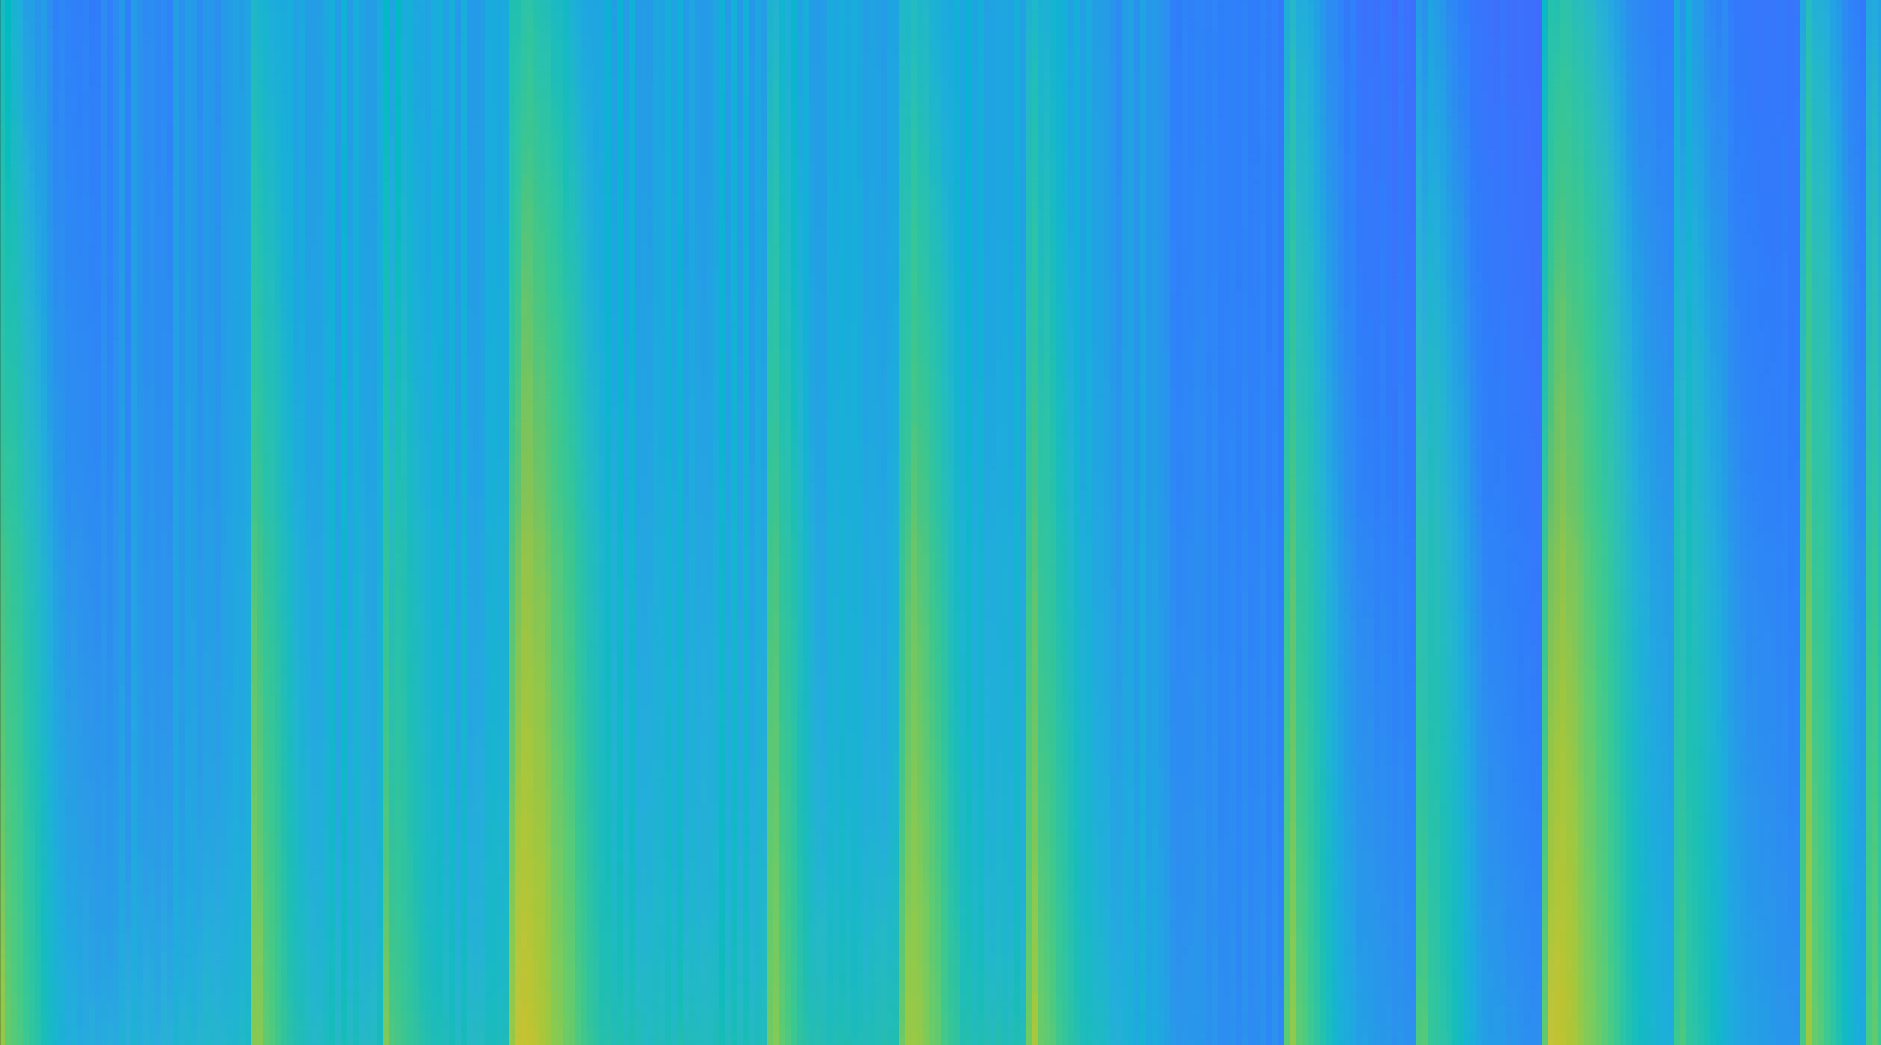
\includegraphics[height=5cm]{../images/medfilter_axis1.png}
		\caption{Mixed spectrogram + vertical median filter}
	\end{figure}
\end{frame}

\begin{frame}
	\frametitle{Median filtering spectrograms}
	Horizontal median filter = ``harmonic separation''
	\begin{figure}
	
\includegraphics[height=5cm]{../images/medfilter_axis2.png}
		\caption{Mixed spectrogram + horizontal median filter}
	\end{figure}
\end{frame}

\begin{frame}
	\frametitle{STFT -- short-time Fourier transform}
	``The STFT is a sequence of Fourier transforms of a windowed signal. STFT provides the time-localized frequency information for situations in which frequency components of a signal vary over time, whereas the standard Fourier transform provides the frequency information averaged over the entire signal time interval'' \footfullcite{timefreq}\\\ \\
	The MATLAB ``spectrogram'' function uses the STFT \footfullcite{specstft}
\end{frame}

\begin{frame}
	\frametitle{STFT -- spectral leakage}
	``The DFT implicitly assumes that the signal is periodic, i.e. that the time series of length N repeats itself infinitely in a cyclic manner. If the frequency of the sinusoidal input signal is not an exact multiple of the frequency resolution, this assumption is not true, and the DFT will see a discontinuity between the last sample and the first sample due to the cyclic continuation. That discontinuity spreads power all across the spectrum.'' \footfullcite{whyoverlap}
\end{frame}

\begin{frame}
	\frametitle{STFT -- spectral leakage}
	\begin{figure}
		\subfloat[Spectral leakage visualization \footfullcite{leakage}]{{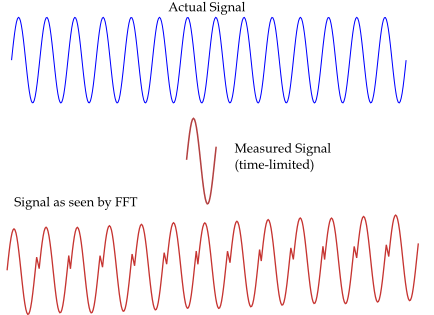
\includegraphics[width=5cm]{../images/spectral_leakage.png} }}
		\hspace{0.2em}
		\subfloat[Tapered von Hann window]{{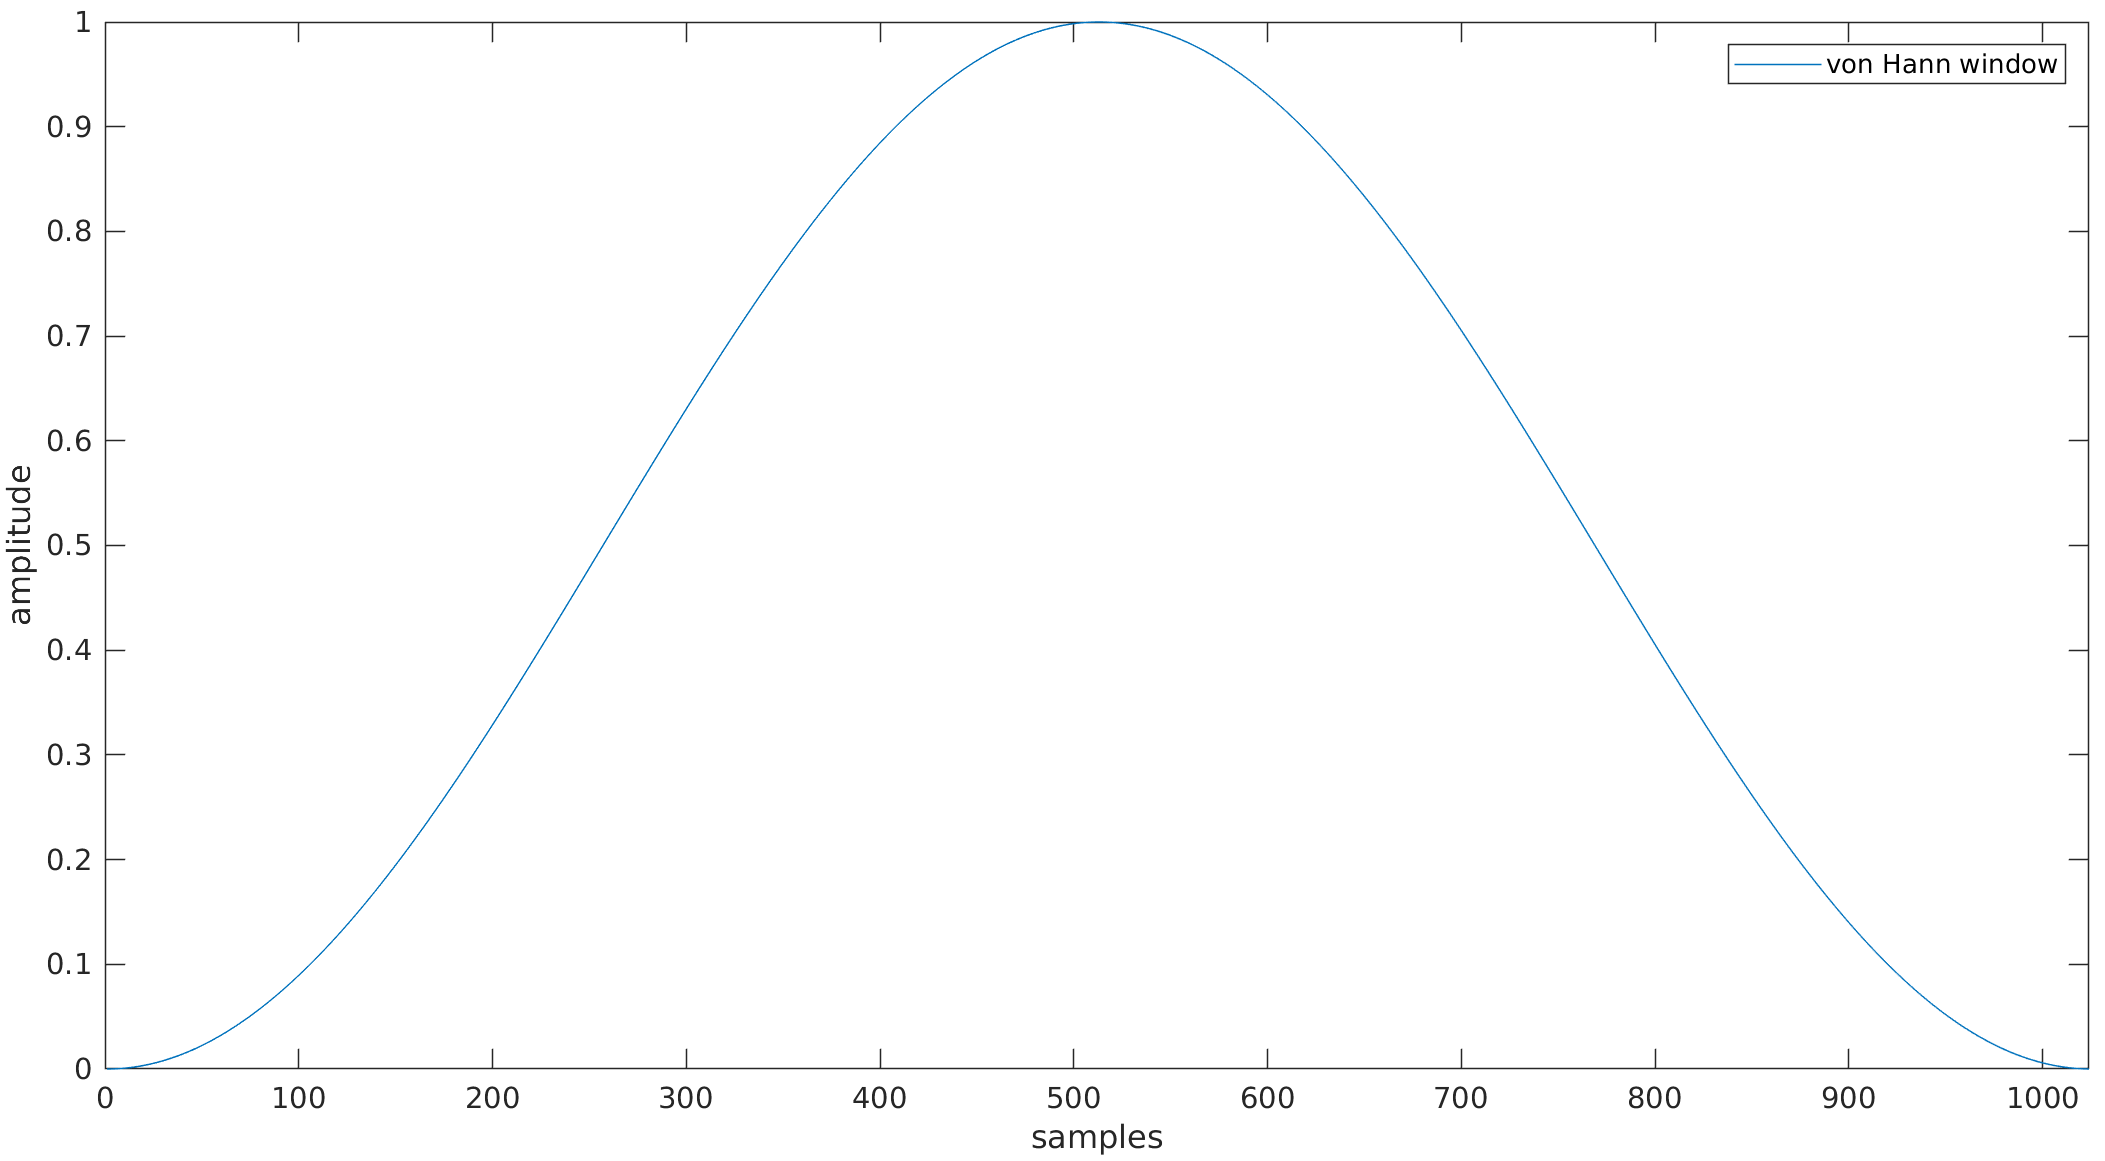
\includegraphics[width=5cm]{../images/hann_taper_window.png} }}
		\caption{Spectral leakage discontinuities and tapered windowing}
	\end{figure}
\end{frame}

\begin{frame}
	\frametitle{STFT -- window + overlap}
The reason there is windowing and overlapping in the STFT is to reduce the effect of spectral leakage. By applying a tapering window, we are losing data at the boundaries of the segment and eliminating the discontinuities of spectral leakage. However, we want segments to overlap to preserve the data that would be lost at the boundaries.
\end{frame}

\begin{frame}
	\frametitle{STFT -- window + overlap}
	\begin{figure}
		\subfloat[Data loss at boundaries]{{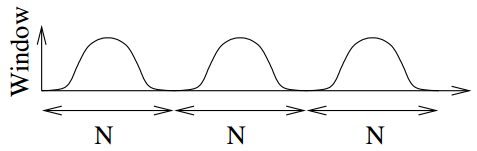
\includegraphics[width=5cm]{../images/whyoverlap1.png} }}
		\hspace{0.2em}
		\subfloat[Overlap to preserve data]{{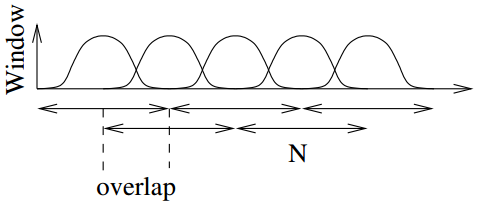
\includegraphics[width=5cm]{../images/whyoverlap2.png} }}
		\caption{Windowing and overlapping}
	\end{figure}
\end{frame}

\begin{frame}
	\frametitle{Time-frequency masking}

Time-frequency masking (T-F masking) is a common technique for source separation \footfullcite{wang2008time}, \footfullcite{timefreq2}.\\
	Create 2-dimensional masks to apply to the time-frequency representation of sound to separate the target signal from the interfering signals. If the mask coefficients are only 0 and 1, this is known as binary masking -- otherwise, the T-F mask is a ratio mask, soft mask, or Wiener filter.
\end{frame}

\begin{frame}
	\frametitle{Fitzgerald 2010 HPSS algorithm}
	Harmonic-percussive source separation based on median filtering\footfullcite{fitzgerald}, pseudocode:
	\vspace{0.75em}
	\begin{enumerate}
		\item $ s = \text{mixed audio}, \hat{S} = \text{STFT}(s), S = \text{abs}(\hat{S}) $
		\item $ H = \text{medianfilter}(S, l_{H}, \text{ax}=2), P = \text{medianfilter}(S, l_{P}, \text{ax}=1) $
		\item $ M_{H} = \frac{H^{p}}{H^{p} + P^{p}}, M_{P} = \frac{P^{p}}{H^{p} + P^{p}} $
		\item $ \hat{H} = \hat{S} \cdot M_{H}, \hat{P} = \hat{S} \cdot M_{P} $
		\item $ h = \text{ISTFT}(\hat{H}), p = \text{ISTFT}(\hat{P}) $
	\end{enumerate}
	Params: $l_{h}$ = $l_{p}$ = 17, $p$th mask power = 2\\
	STFT params: frame size = window size = 1024, overlap = 512, window = sqrt(hann)
\end{frame}

\begin{frame}
	\frametitle{Fitzgerald 2010 HPSS algorithm}
	What is \[ M_{H} = \frac{H^{p}}{H^{p} + P^{p}}, M_{P} = \frac{P^{p}}{H^{p} + P^{p}} \]
	Soft mask, Wiener filter. Used for image denoising.\footfullcite{wienernoise}\\
	Consider that the mixed spectrogram is a sum of harmonic and percussive components:
	\[ \hat{S} = \hat{H} + \hat{P} \]
	We ``denoise'' P from S using $M_{H}$ to get H, and vice-versa
\end{frame}

\begin{frame}
	\frametitle{Mixed sound}
	\href{run:../audio/mixed.wav}{Recall from earlier}\
	\begin{figure}
	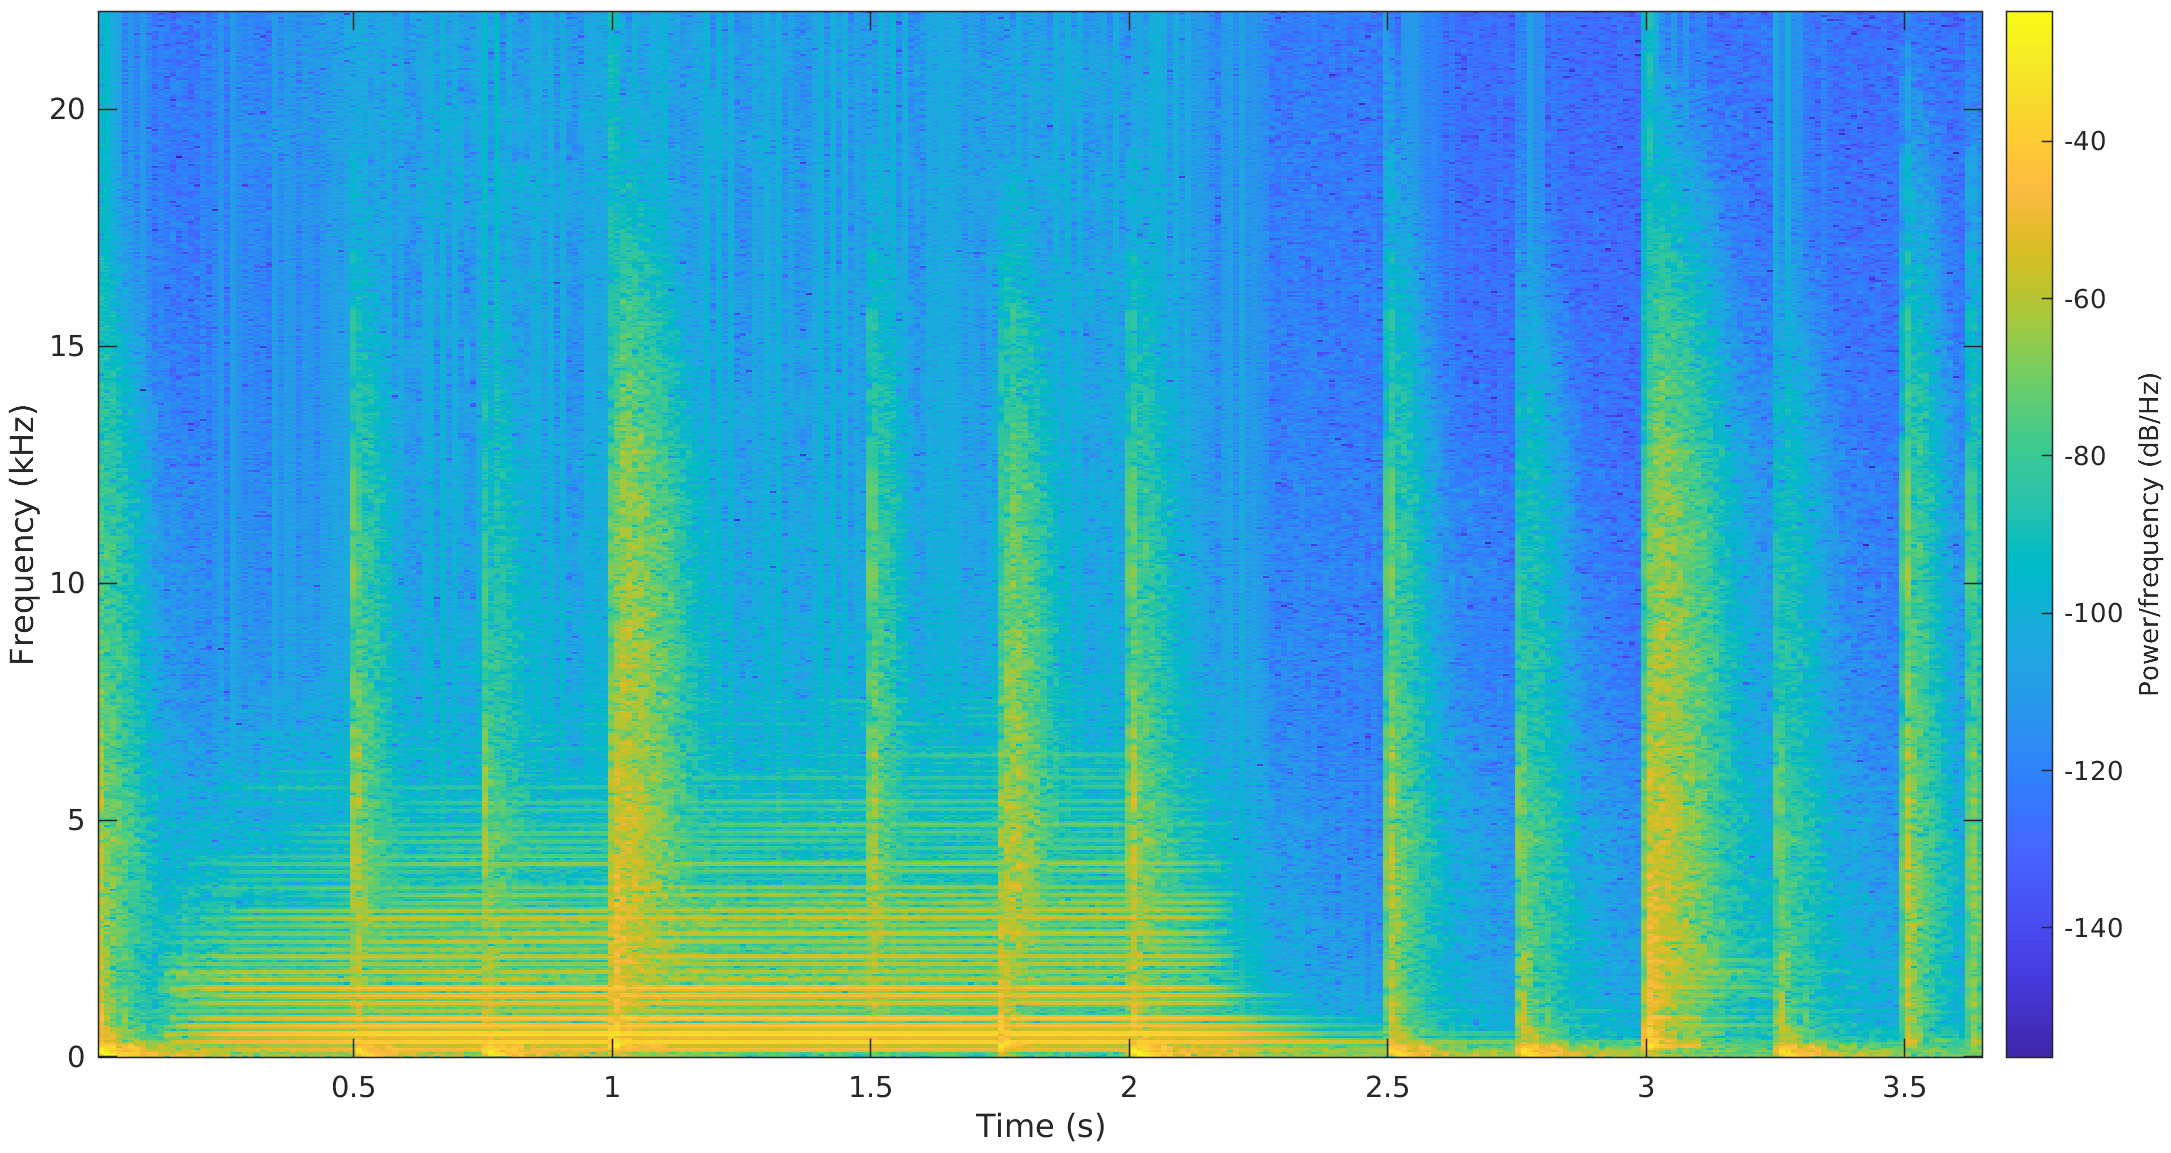
\includegraphics[height=5cm]{../images/mixedspecgram.png}
		\caption{Mixed spectrogram}
	\end{figure}
\end{frame}

\begin{frame}
	\frametitle{Fitzgerald 2010 HPSS algorithm}
	\begin{figure}
	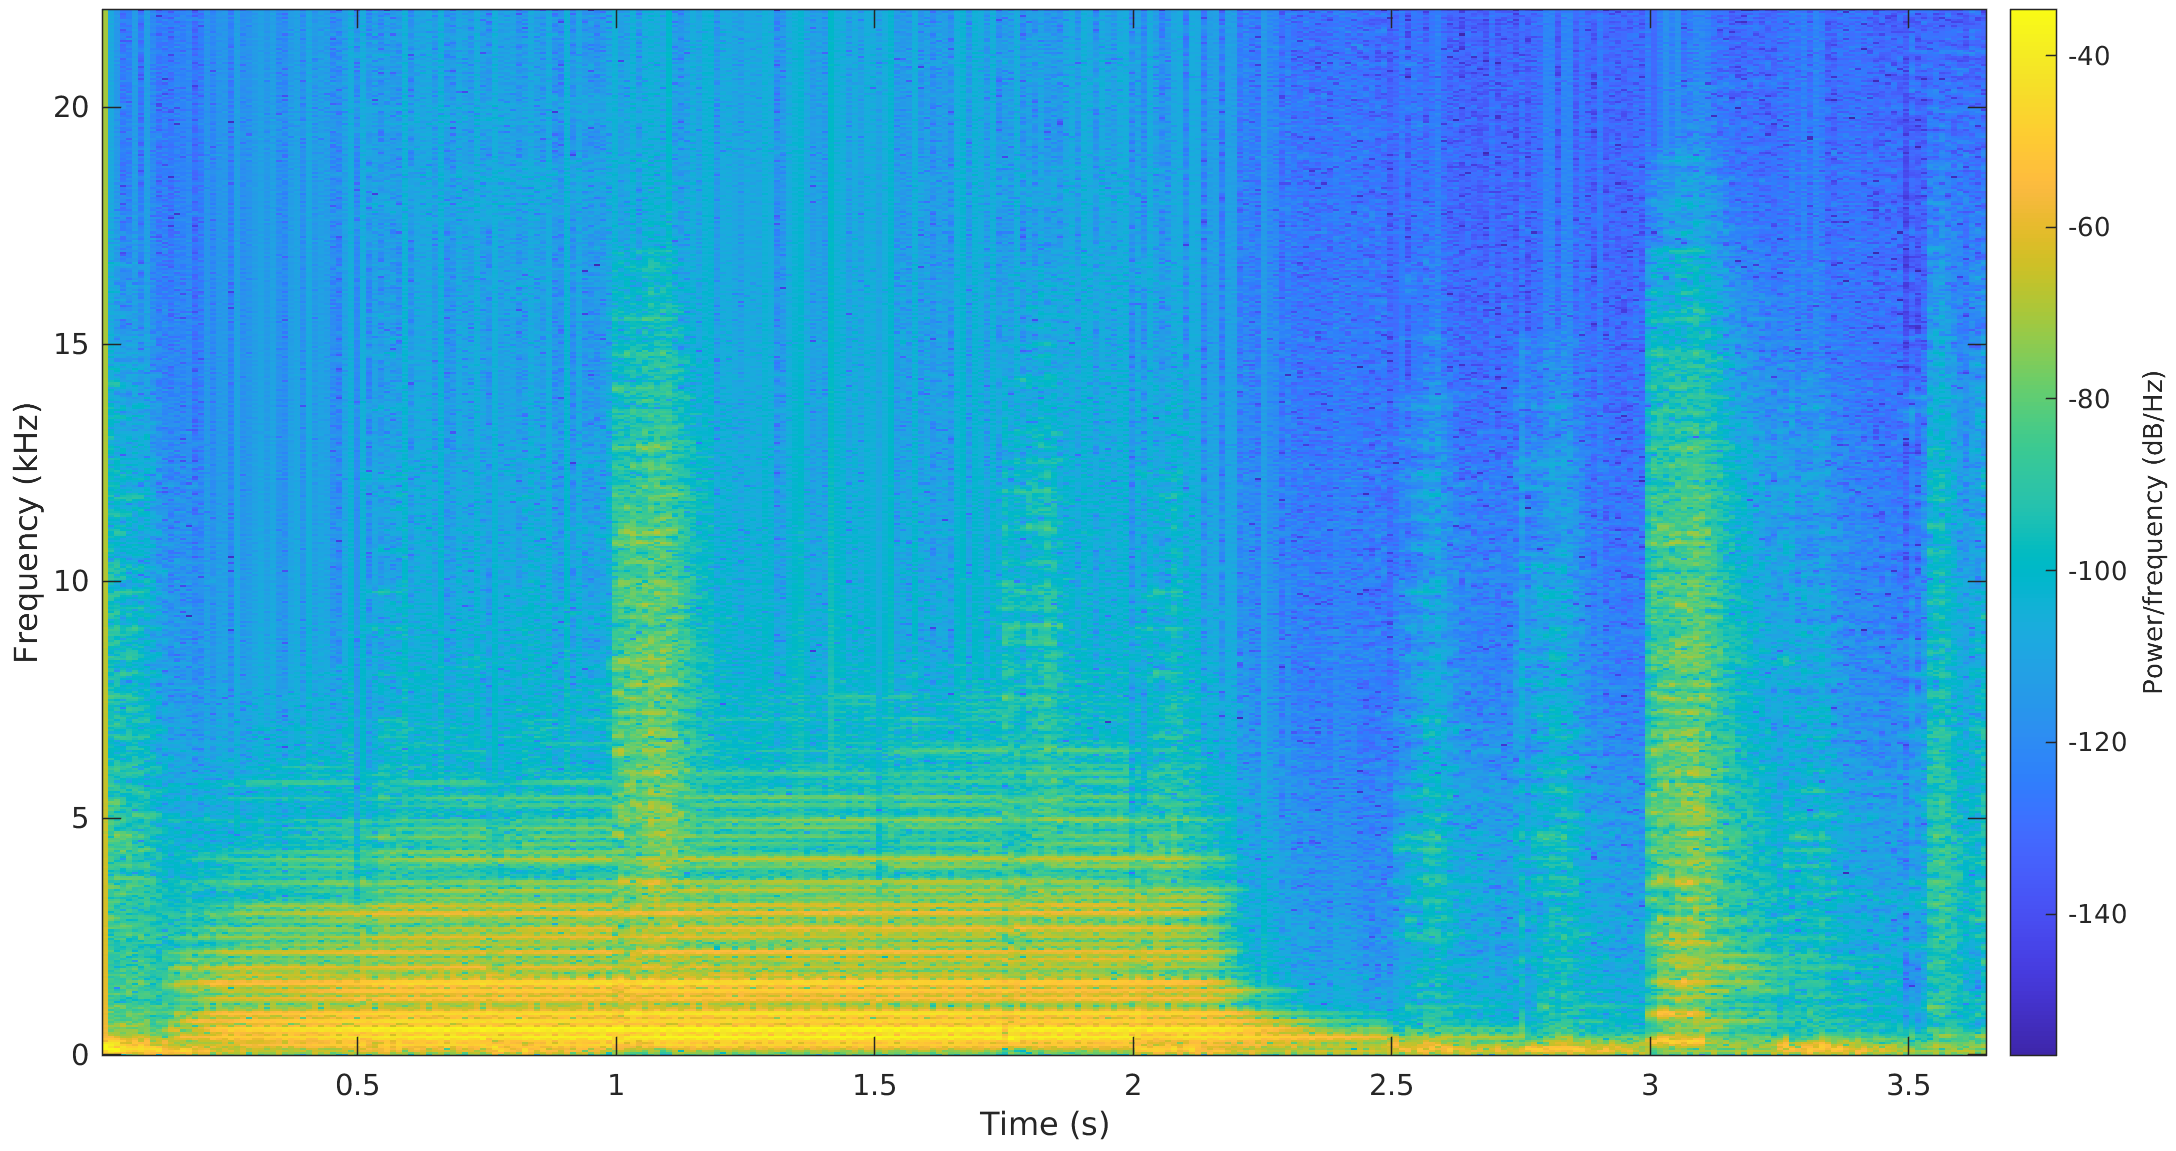
\includegraphics[height=5cm]{../images/harm_soft.png}
		\caption{Separated harmonic spectrogram}
	\end{figure}
\end{frame}

\begin{frame}
	\frametitle{Fitzgerald 2010 HPSS algorithm}
	\href{run:../audio/harm_fitzgerald_nonrealtime.wav}{Click to listen}\\
	\begin{figure}
	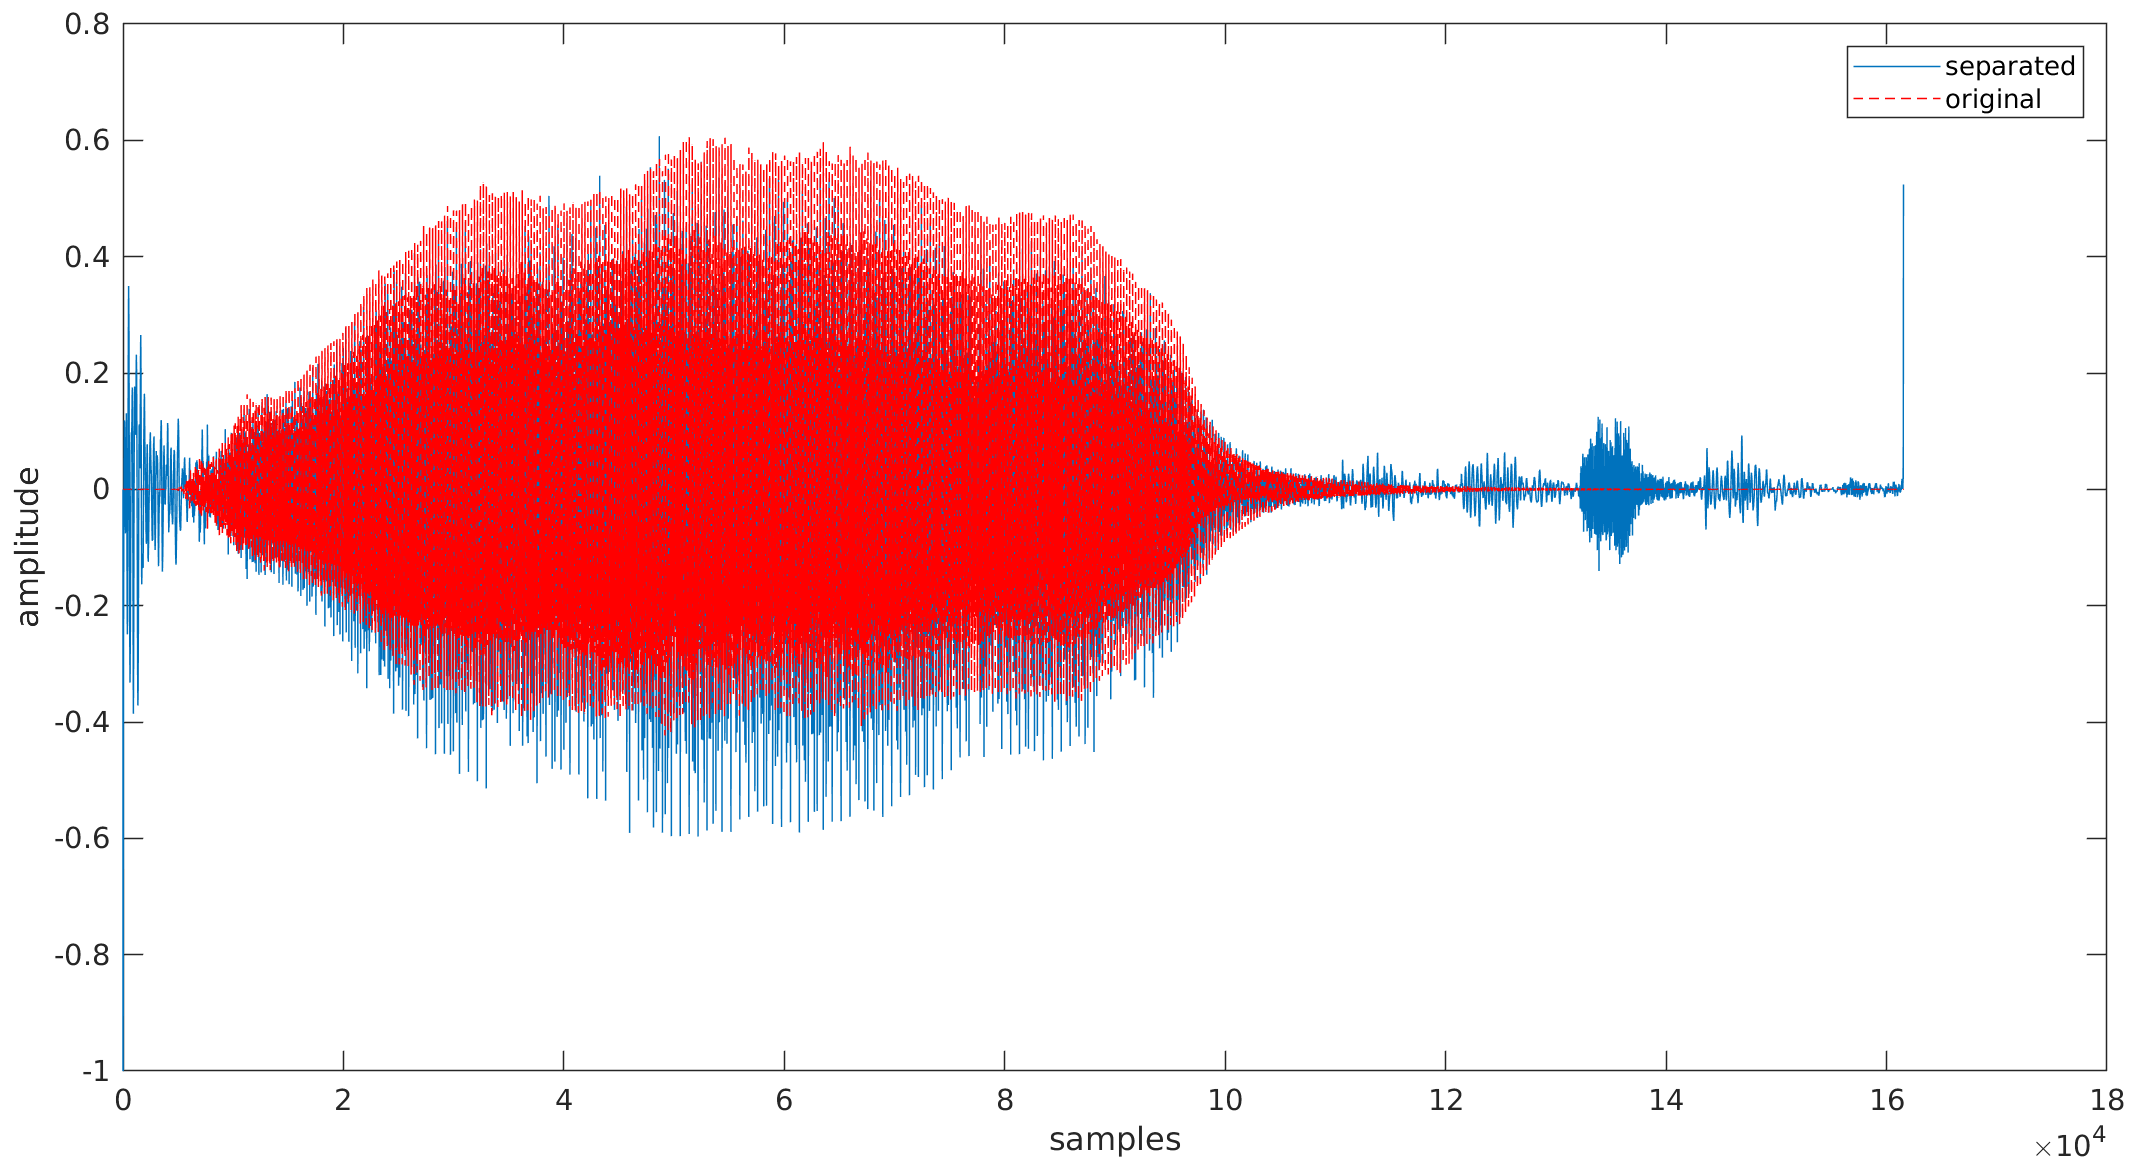
\includegraphics[height=5cm]{../images/harm_fitzgerald_cmp.png}
		\caption{Harmonic waveform comparison}
	\end{figure}
\end{frame}

\begin{frame}
	\frametitle{Fitzgerald 2010 HPSS algorithm}
	\begin{figure}
	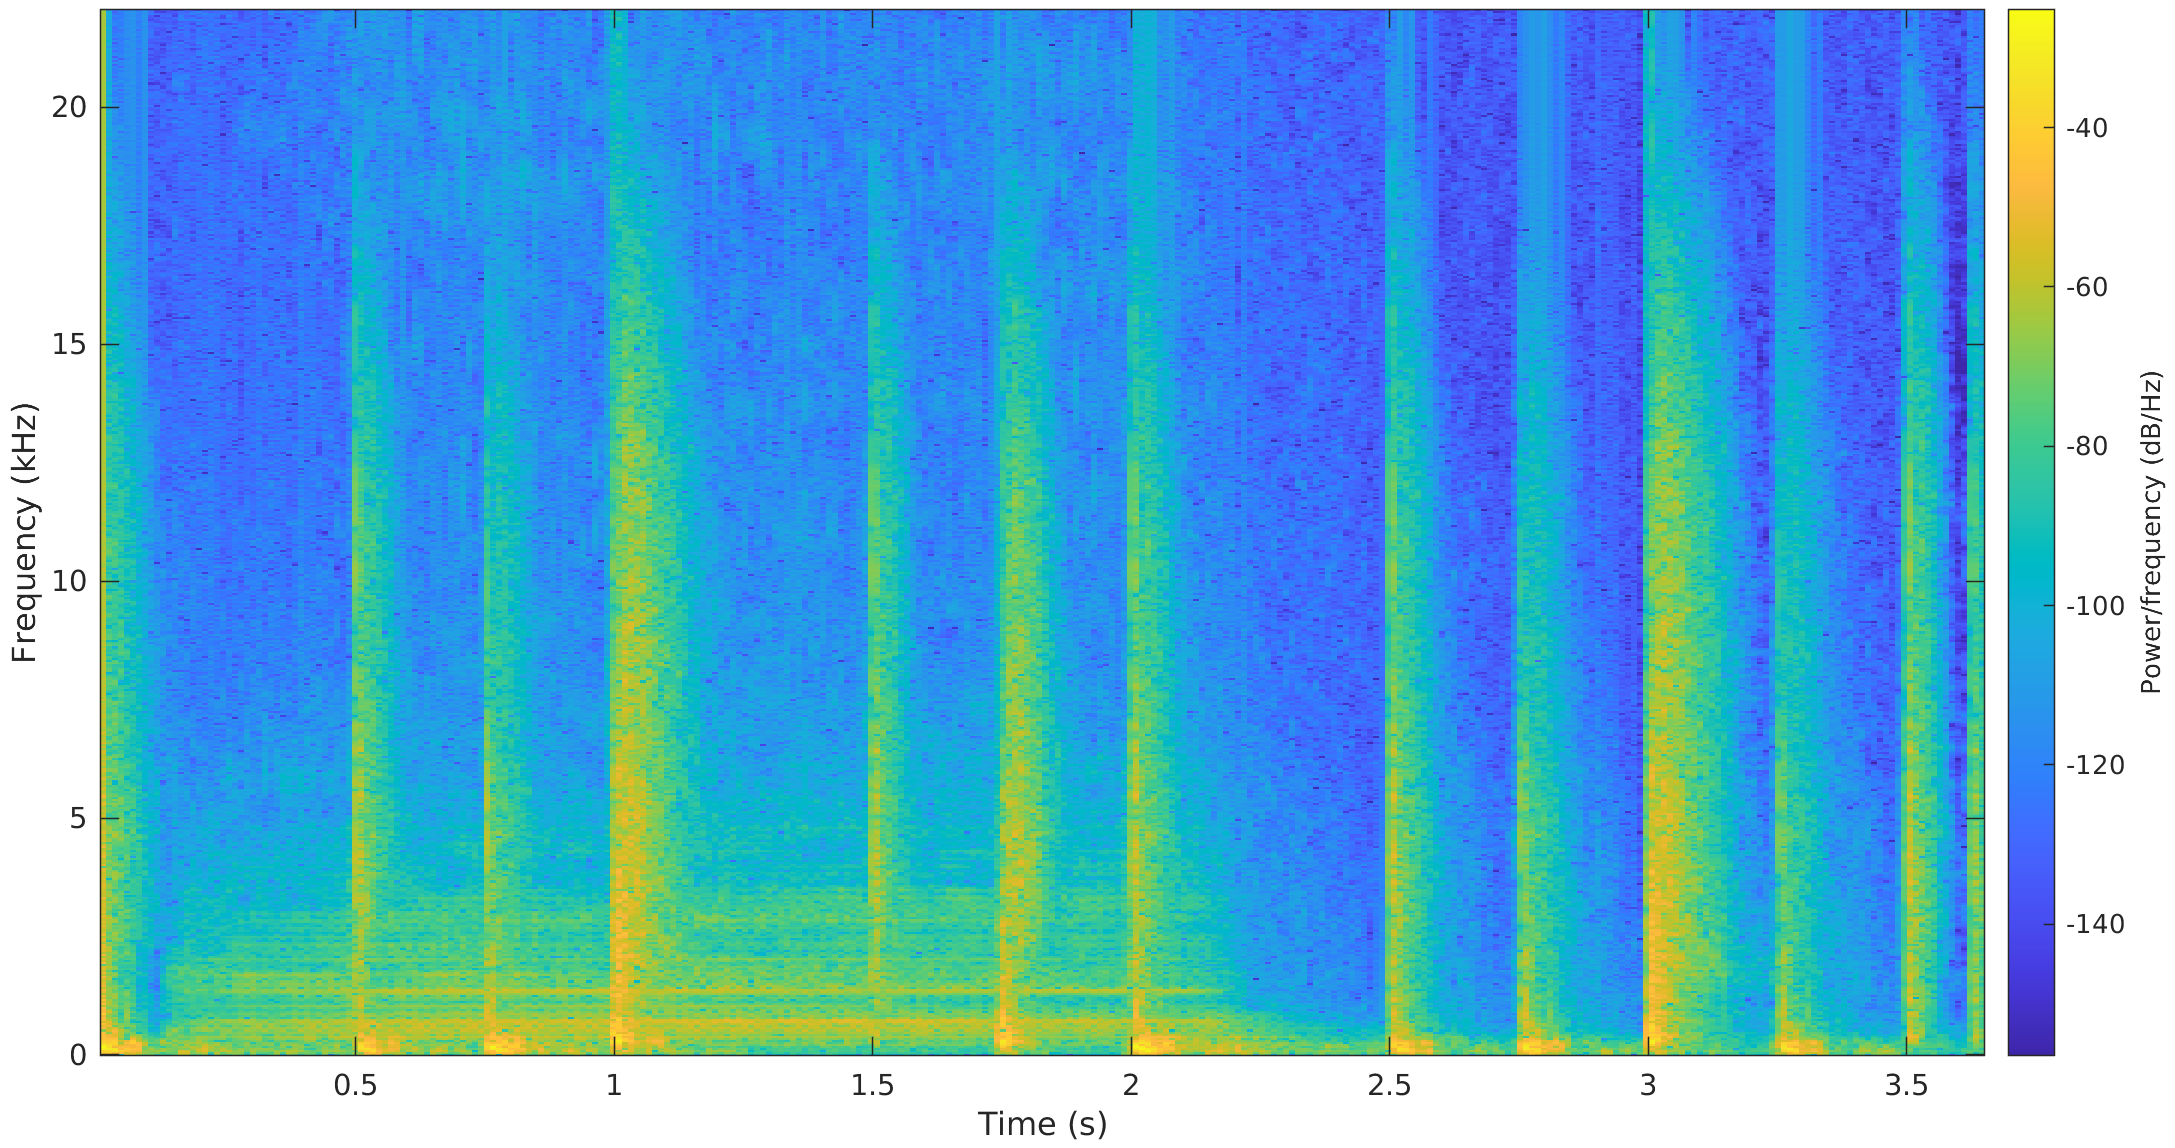
\includegraphics[height=5cm]{../images/perc_soft.png}
		\caption{Separated percussive spectrogram}
	\end{figure}
\end{frame}

\begin{frame}
	\frametitle{Fitzgerald 2010 HPSS algorithm}
	\href{run:../audio/perc_fitzgerald_nonrealtime.wav}{Click to listen}\\
	\begin{figure}
	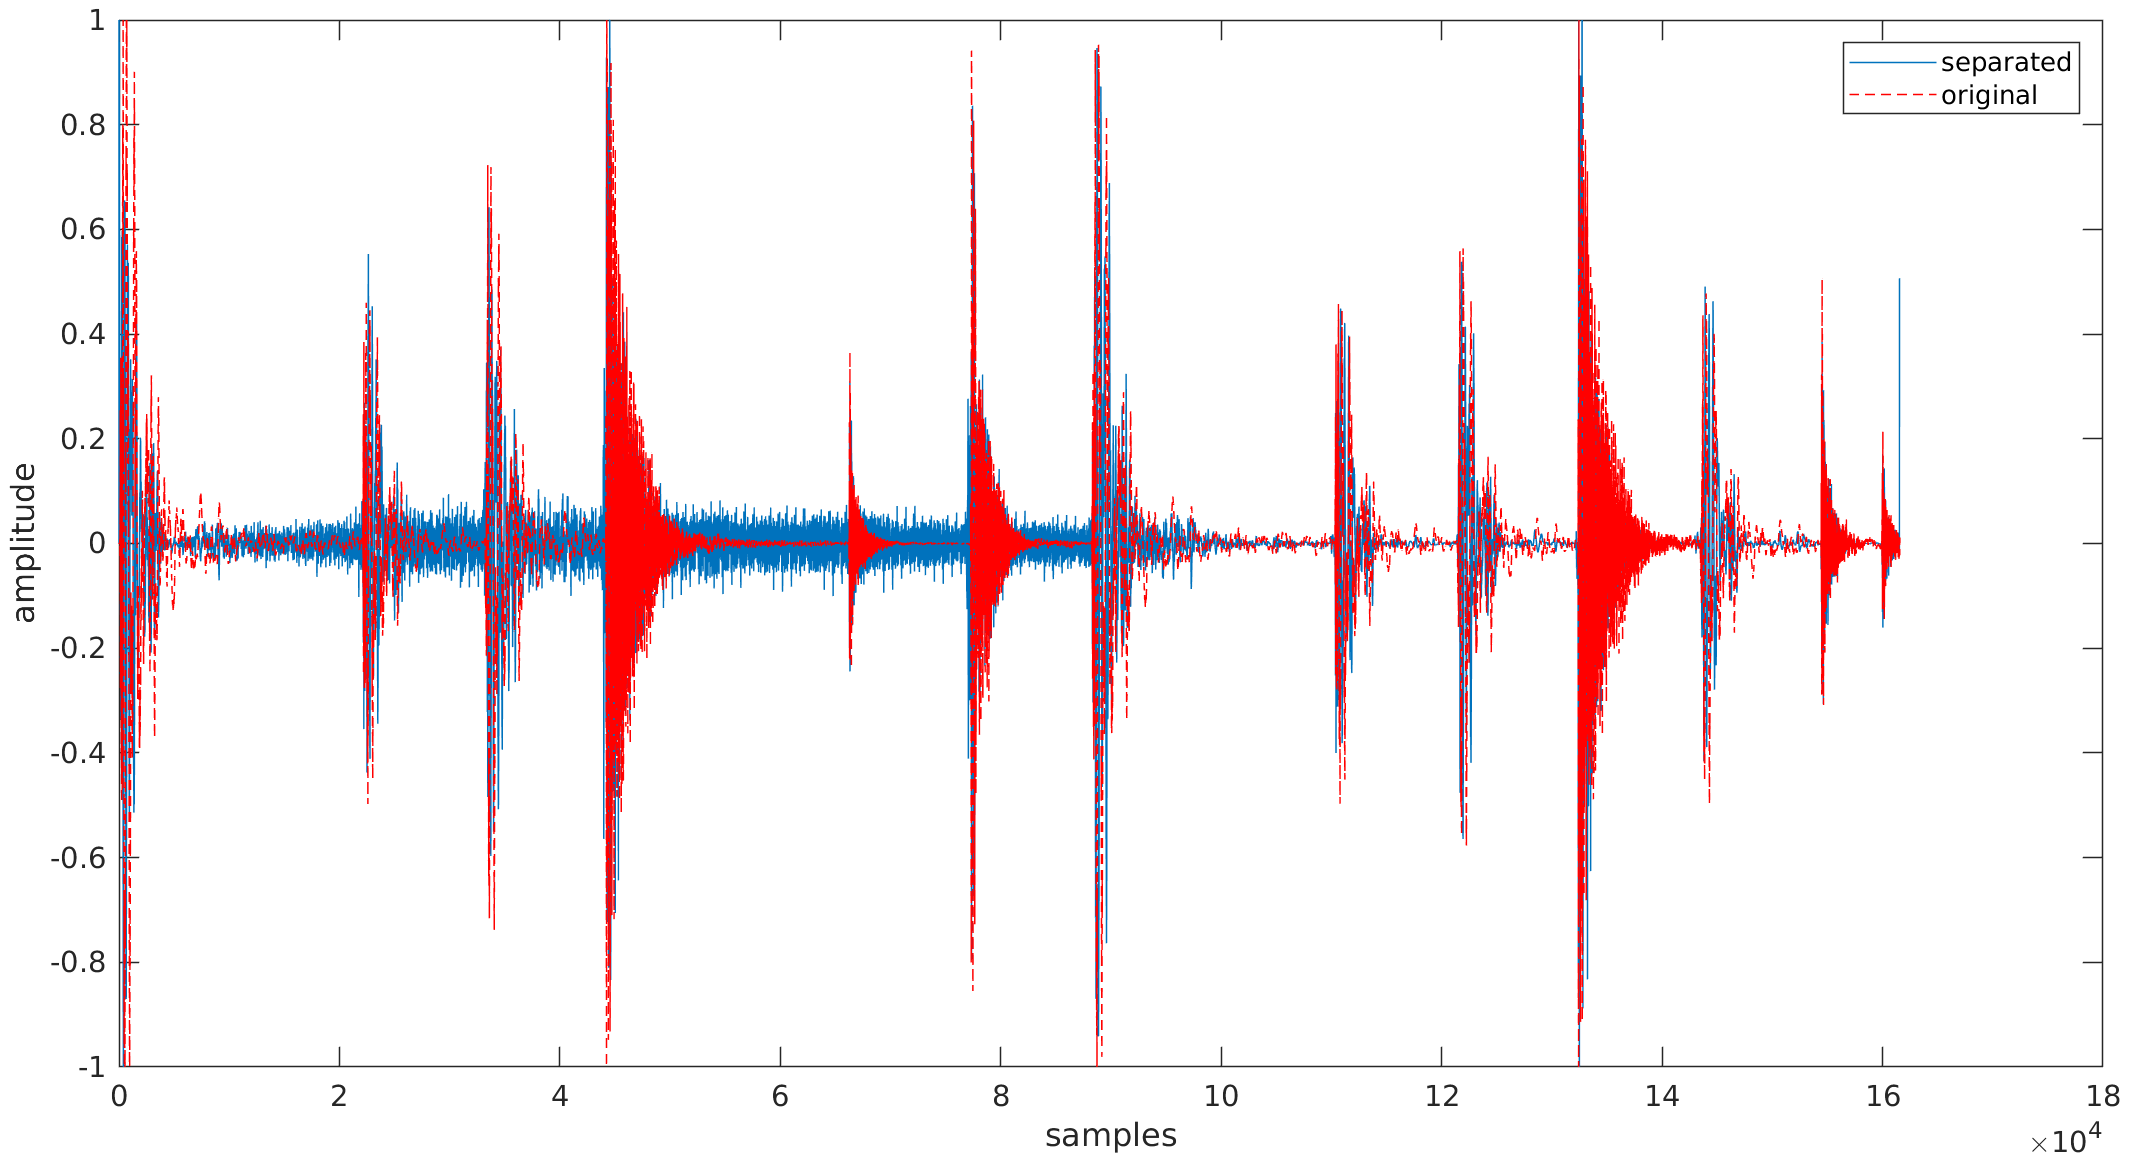
\includegraphics[height=5cm]{../images/perc_fitzgerald_cmp.png}
		\caption{Percussive waveform comparison}
	\end{figure}
\end{frame}

\begin{frame}
	\frametitle{Driedger et al. 2014 improvement}
	New component, the residual -- neither harmonic nor percussive\footfullcite{driedger}
	\[ \hat{S} = \hat{H} + \hat{P} + \hat{X} \]
	Introduced with parameter $beta$, the \textit{separation factor}\\
	Previous soft masks now become binary masks
	\[ M_{H} = \frac{H}{P + \epsilon} > \beta, M_{P} = \frac{P}{H + \epsilon} \ge \beta \]
	Stronger separation of H and P even if we don't care about X. Recommended $\beta$ = 2.
\end{frame}

\begin{frame}
	\frametitle{Mixed sound}
	\href{run:../audio/mixed.wav}{Recall from earlier}\
	\begin{figure}
	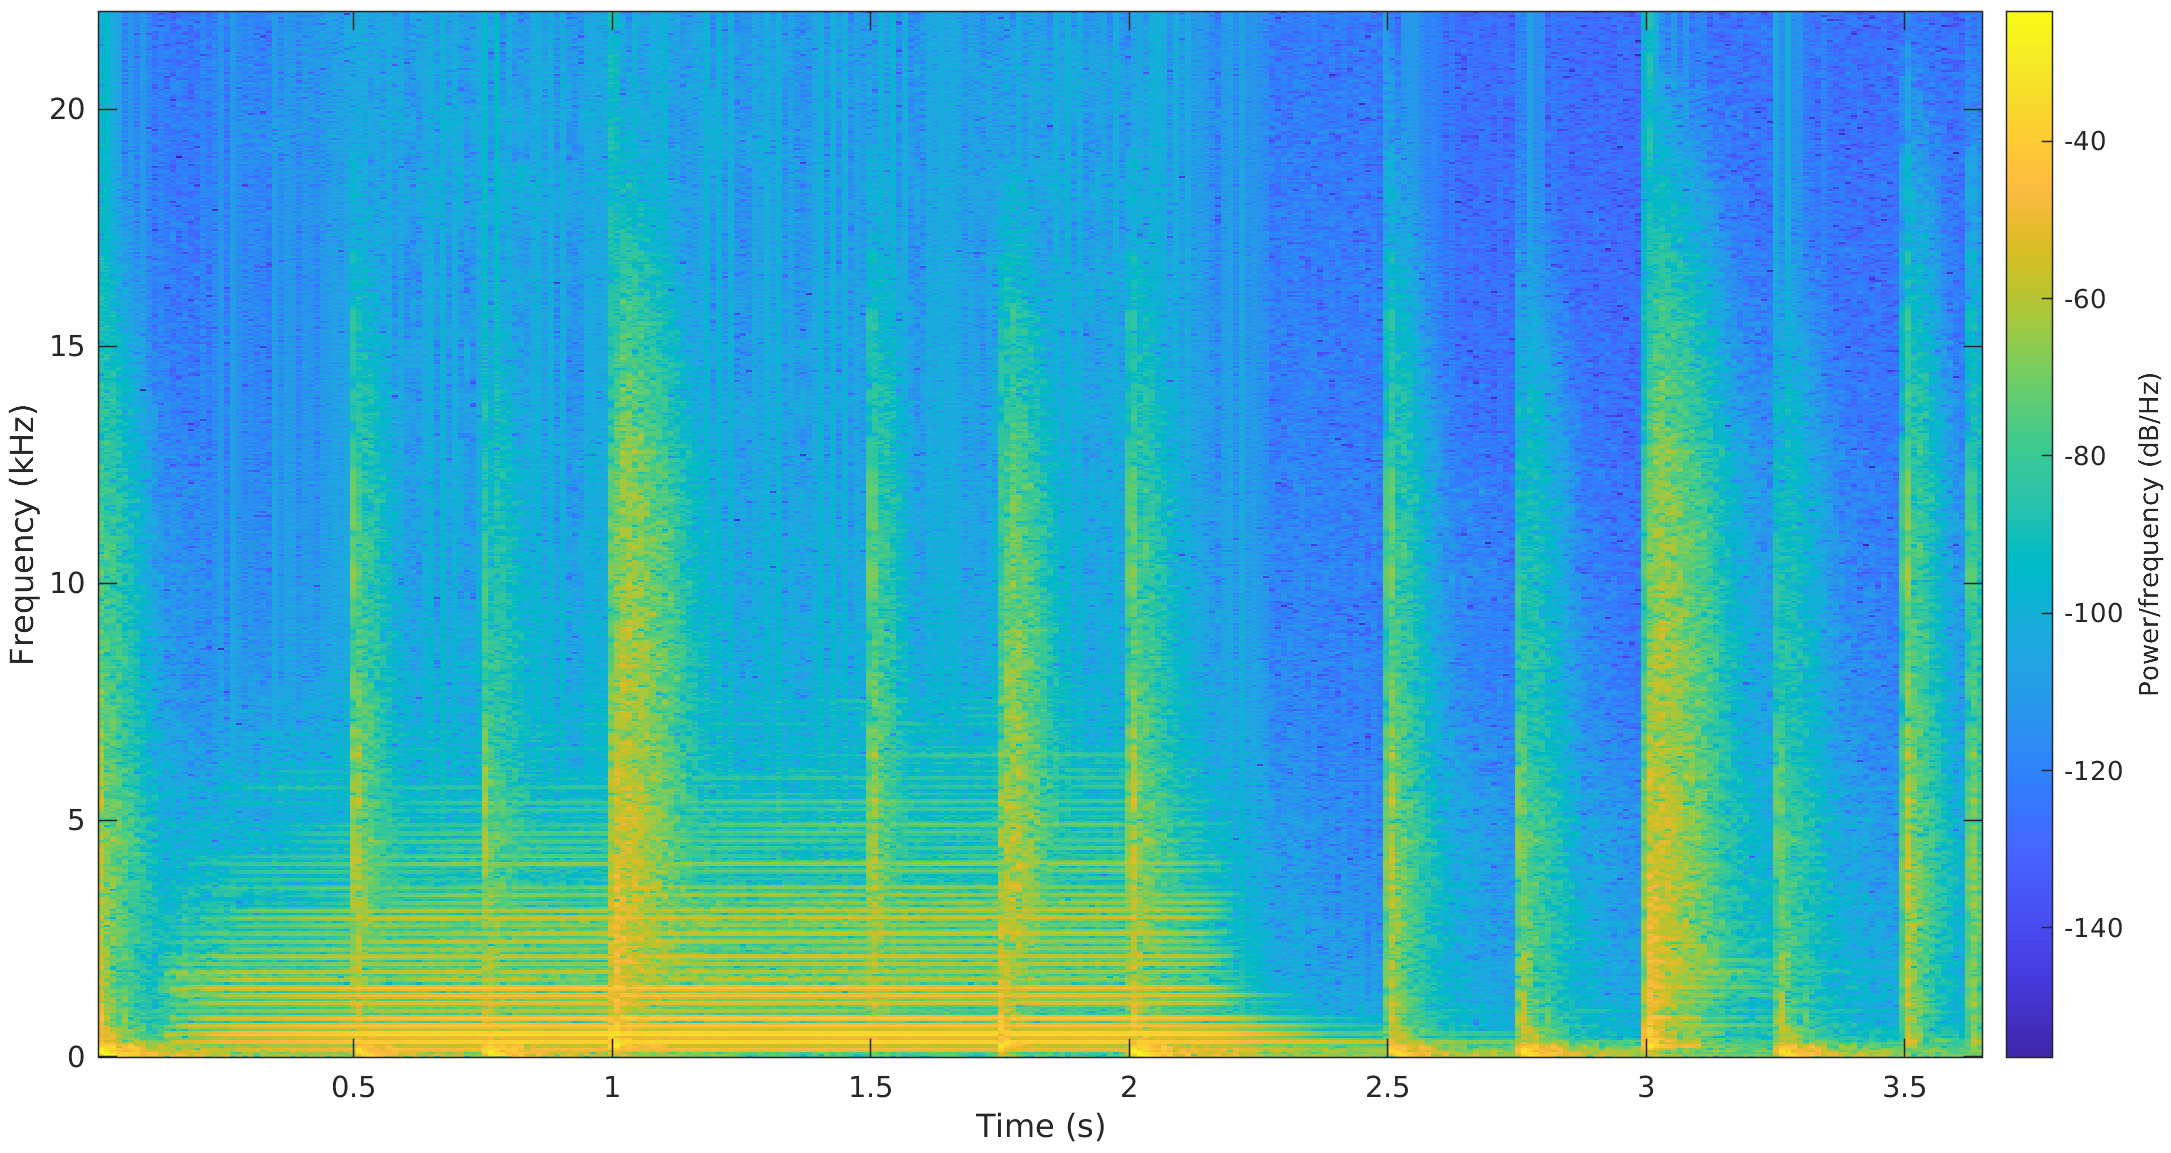
\includegraphics[height=5cm]{../images/mixedspecgram.png}
		\caption{Mixed spectrogram}
	\end{figure}
\end{frame}

\begin{frame}
	\frametitle{Driedger et al. 2014 improvement}
	\begin{figure}
	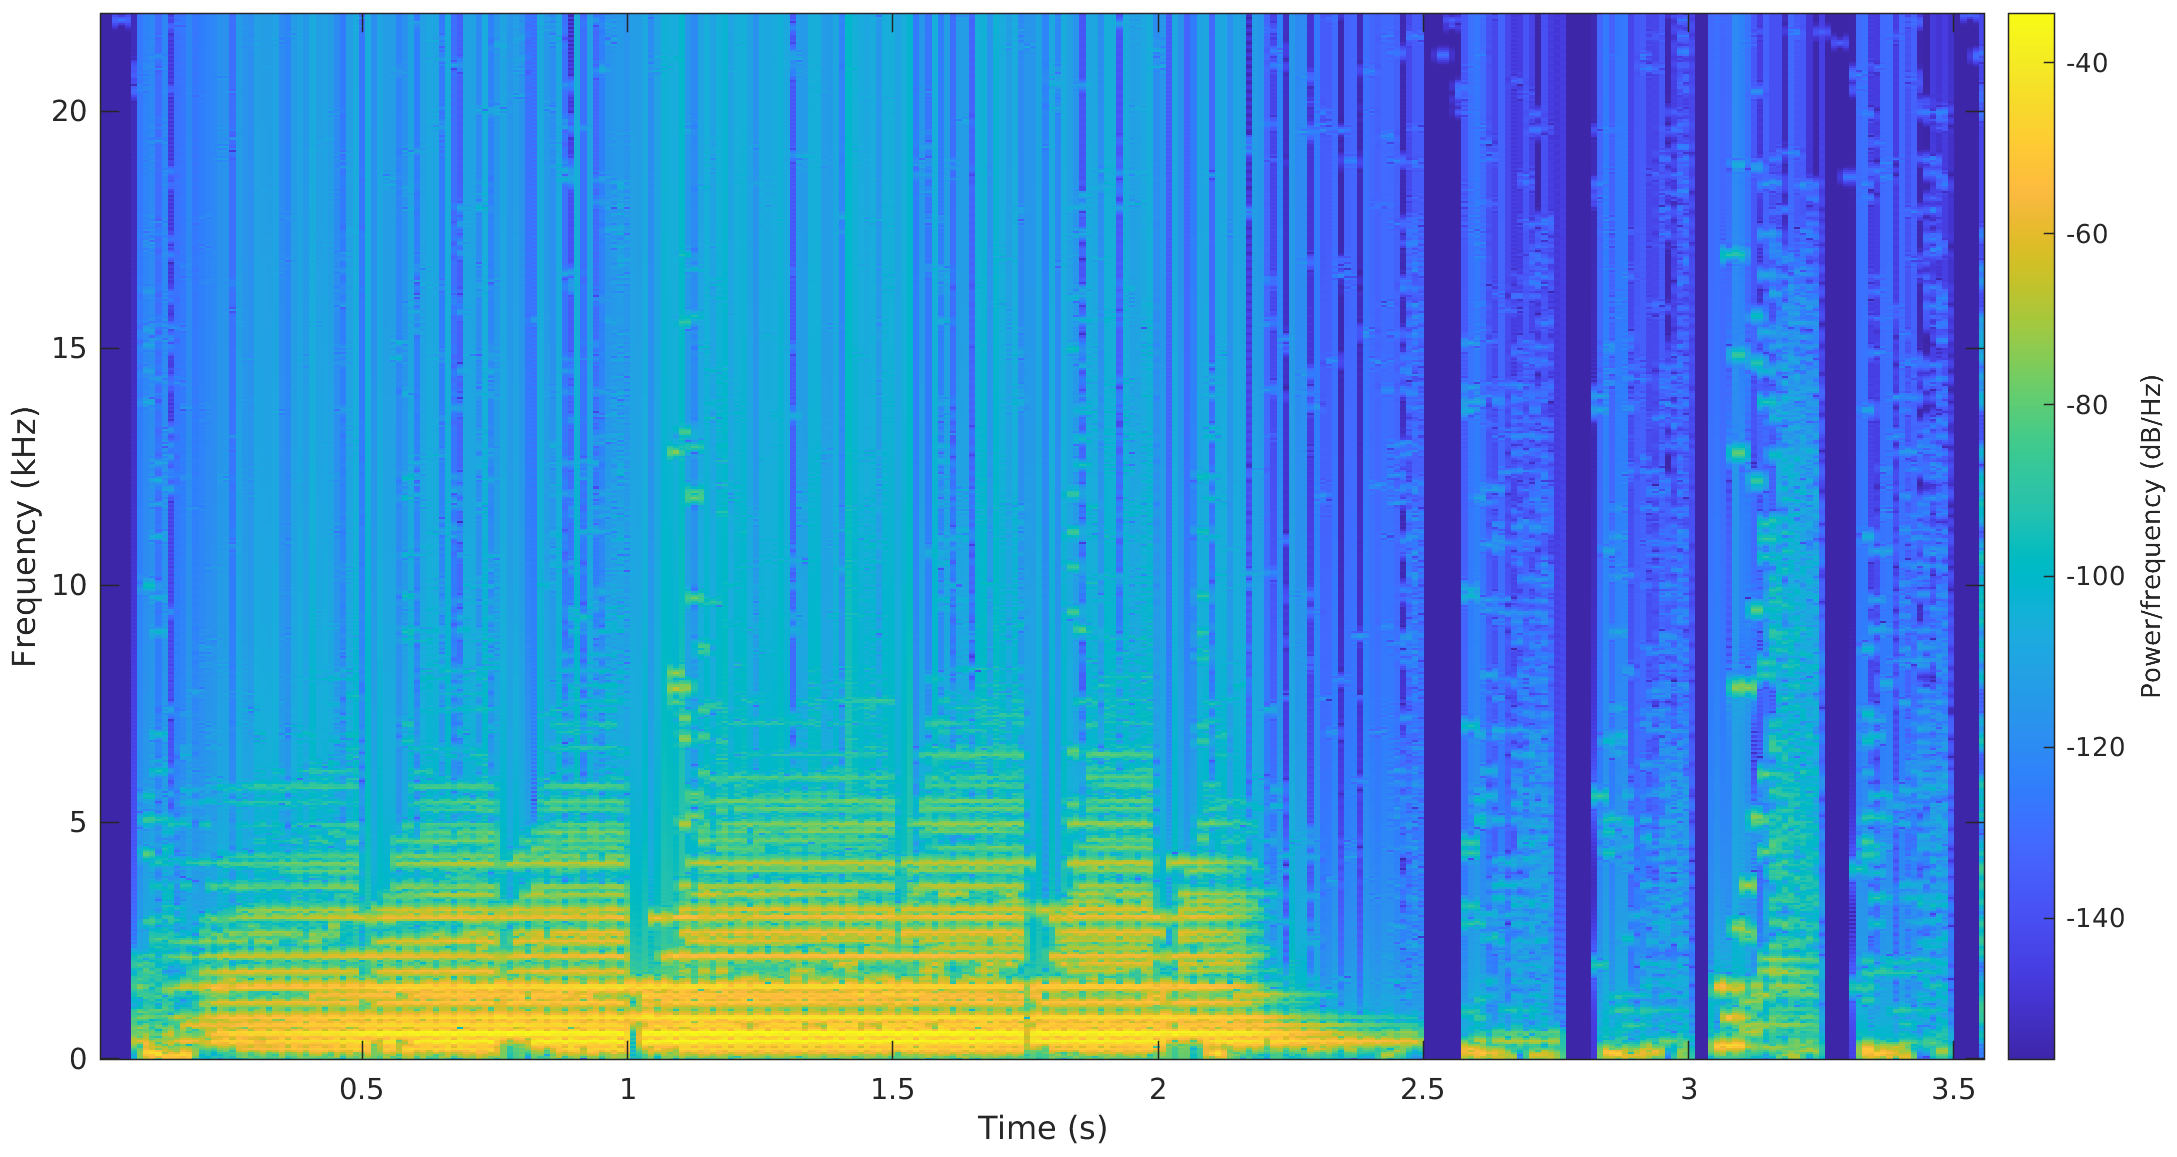
\includegraphics[height=5cm]{../images/harm_binary.png}
		\caption{Separated harmonic spectrogram}
	\end{figure}
\end{frame}

\begin{frame}
	\frametitle{Driedger et al. 2014 improvement}
	\href{run:../audio/harm_driedger_nonrealtime.wav}{Click to listen}\\
	Note the audible silences where percussion was removed.
	\begin{figure}
	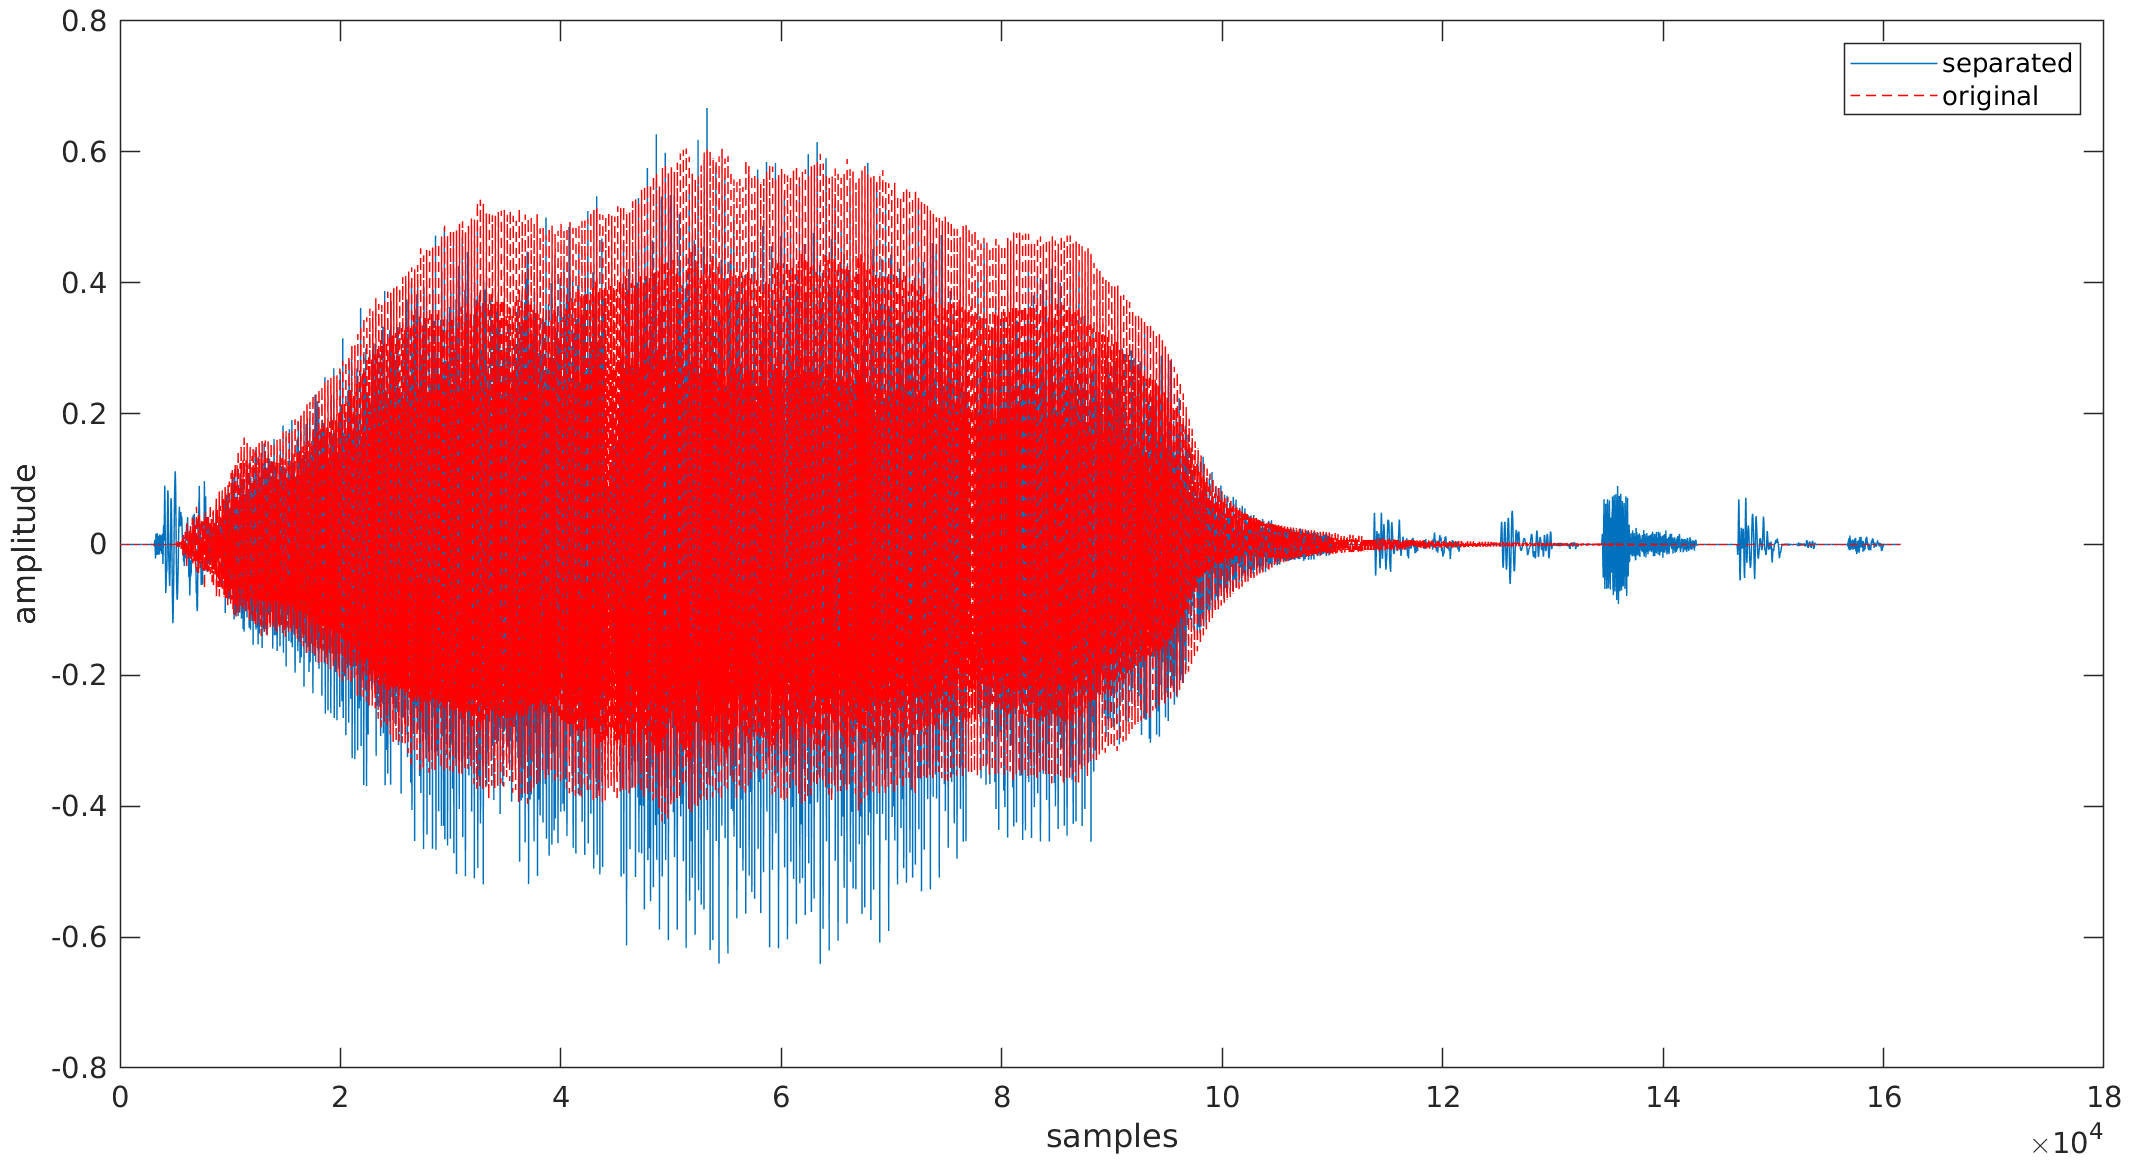
\includegraphics[height=5cm]{../images/harm_driedger_cmp.png}
		\caption{Harmonic waveform comparison}
	\end{figure}
\end{frame}

\begin{frame}
	\frametitle{Driedger et al. 2014 improvement}
	\begin{figure}
	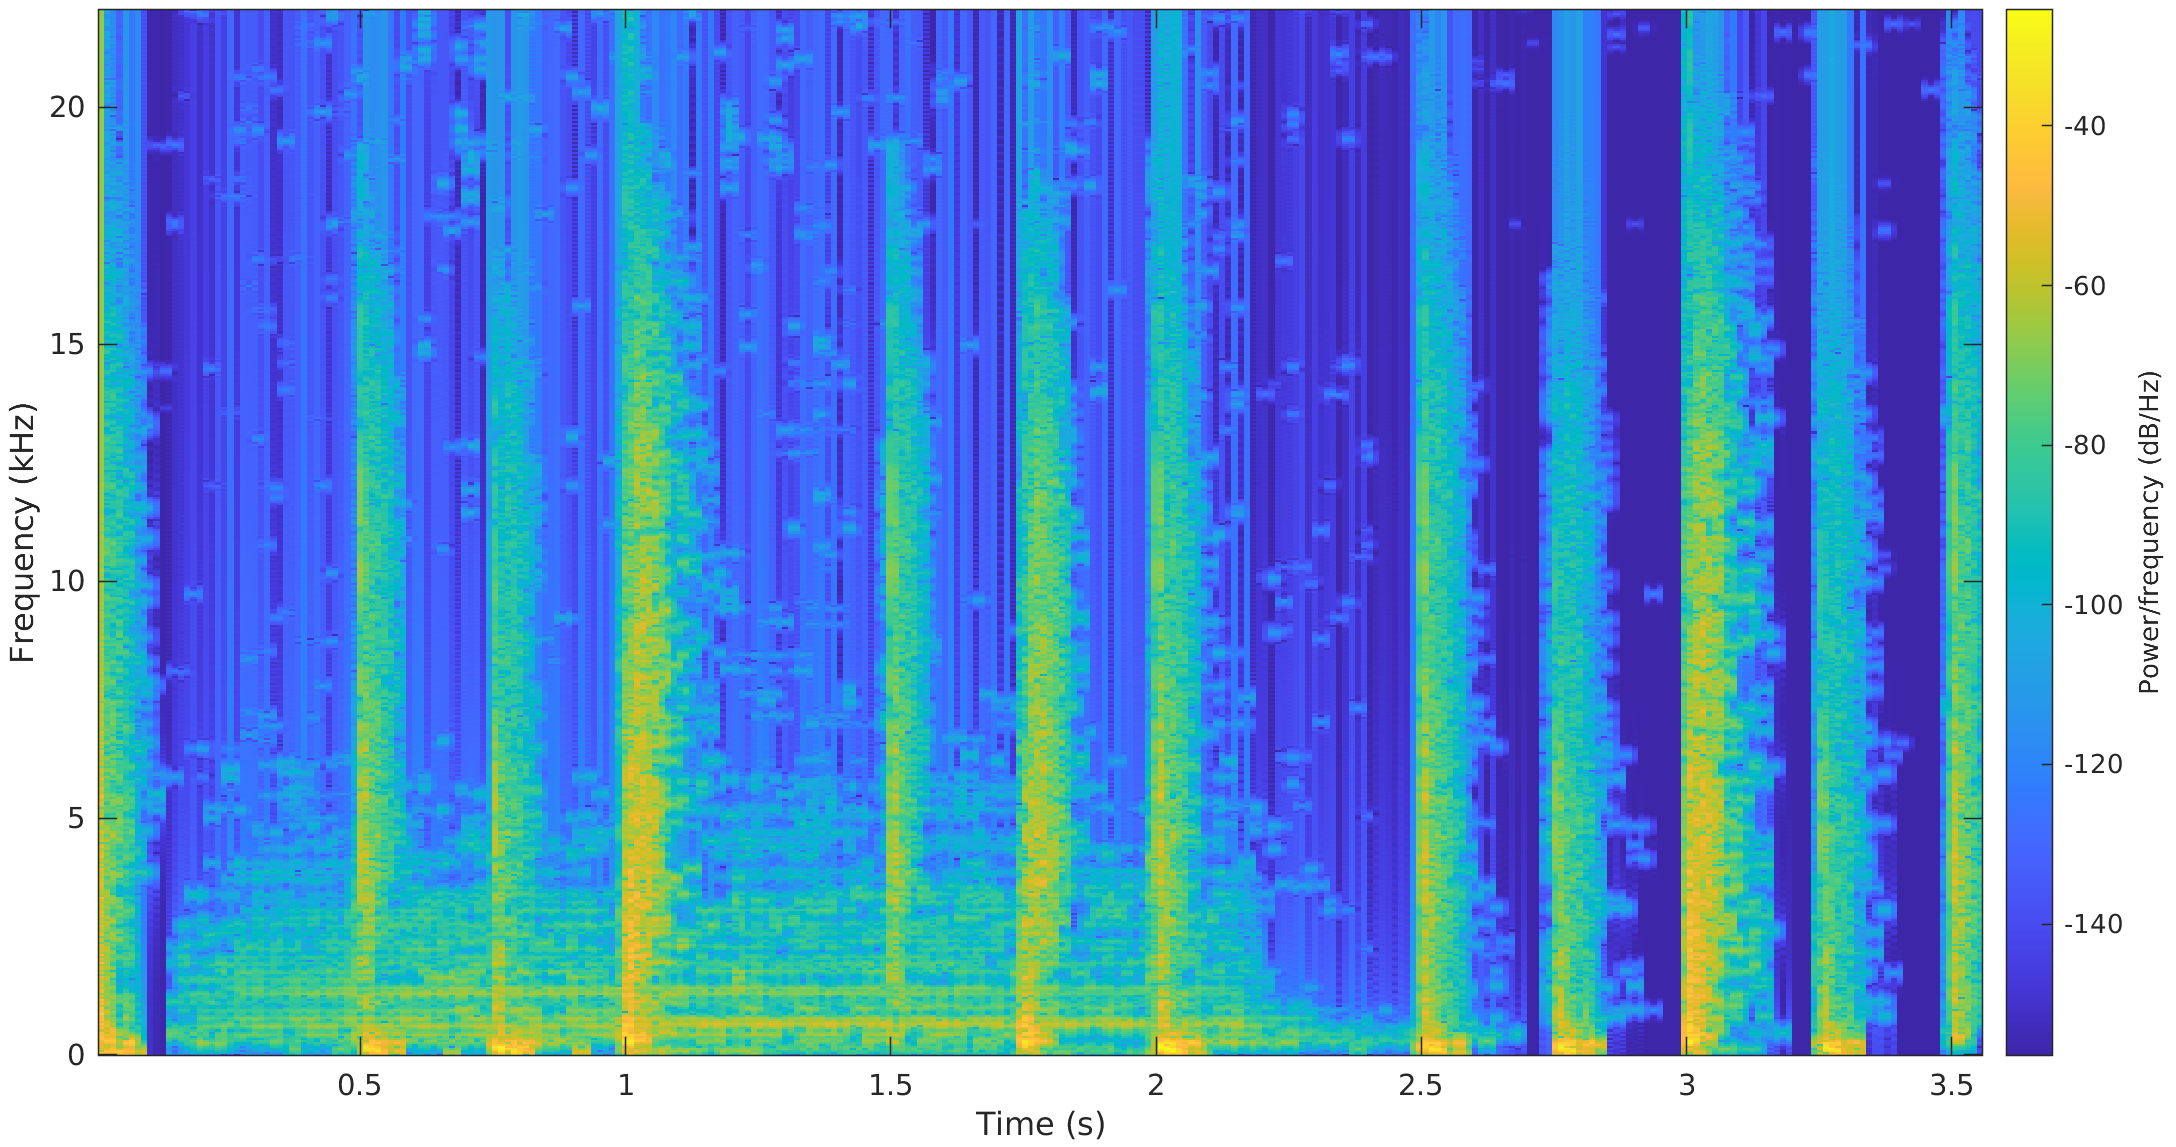
\includegraphics[height=5cm]{../images/perc_binary.png}
		\caption{Separated percussive spectrogram}
	\end{figure}
\end{frame}

\begin{frame}
	\frametitle{Driedger et al. 2014 improvement}
	\href{run:../audio/perc_driedger_nonrealtime.wav}{Click to listen}\\
	\begin{figure}
	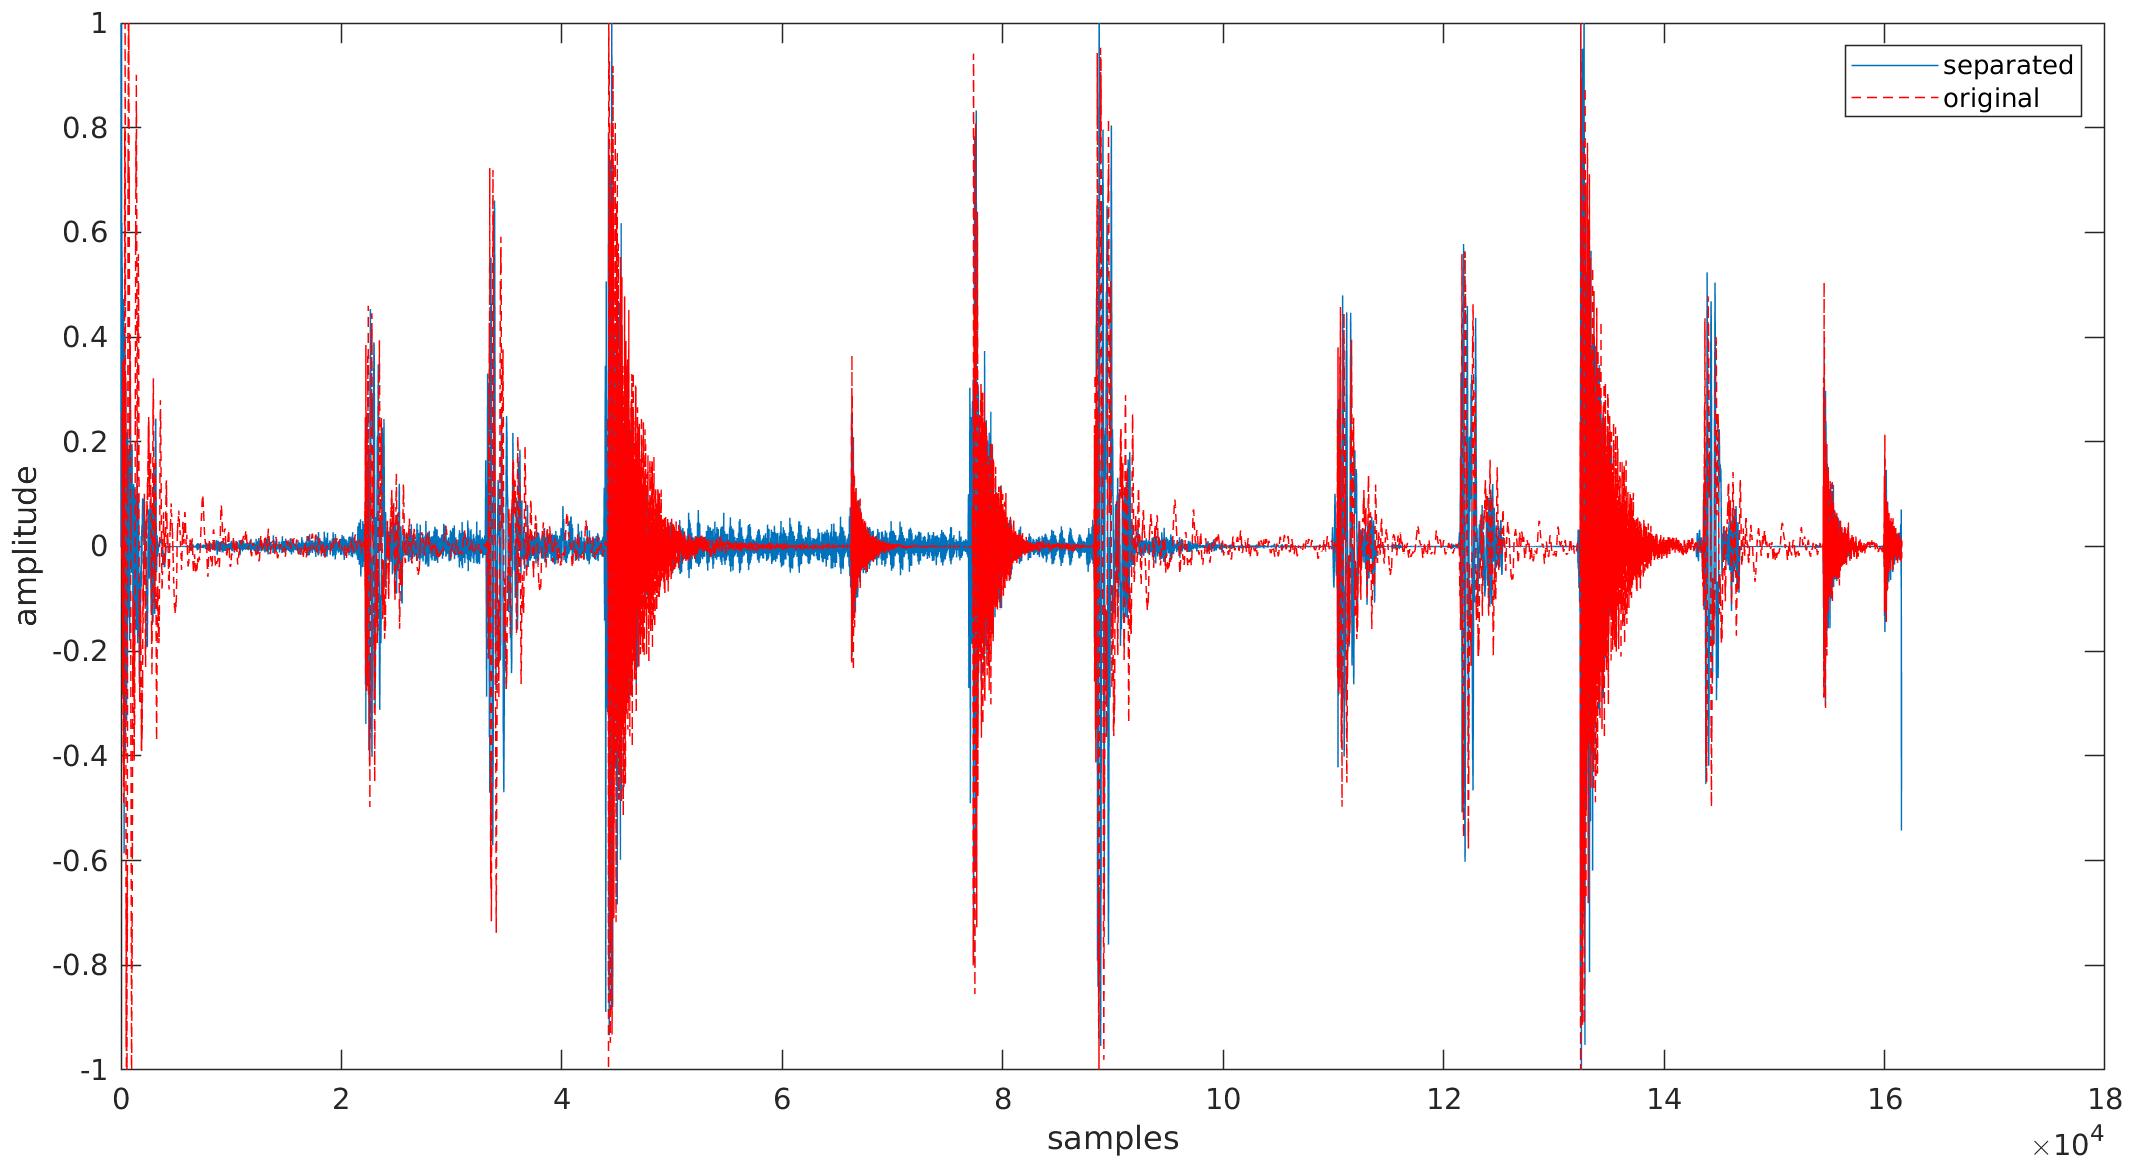
\includegraphics[height=5cm]{../images/perc_driedger_cmp.png}
		\caption{Percussive waveform comparison}
	\end{figure}
\end{frame}

\begin{frame}
	\frametitle{Implementation details 1}
	STFT parameters: square-root von Hann window with $L = 1024$, \textit{overlap} = $512$, \textit{NFFT} = $2048$\footfullcite{god}\\\ \\
	Window and overlap verified to be COLA (Constant Overlap-Add)-compliant with the ``iscola'' function in MATLAB \footfullcite{cola} -- ``ensure that the inverse short-time Fourier transform results in perfect reconstruction for nonmodified spectra.''
\end{frame}

\begin{frame}[fragile]
	\frametitle{Implementation details 2}
	The masks are computed with the magnitude of half of the STFT:
	\begin{small}
	\begin{verbatim}
	    halfIdx = 1:ceil(size(S,1)/2); % only half the STFT matters
	    Shalf = S(halfIdx, :);
	    Smag = abs(Shalf); % use the magnitude STFT for creating masks
	\end{verbatim}
	\end{small}
	Half of the DFT is redundant. Magnitude has more important information than phase for the human ear \footfullcite{zafar}.
\end{frame}

\begin{frame}
	\frametitle{STFT, ISTFT}
	\begin{figure}
	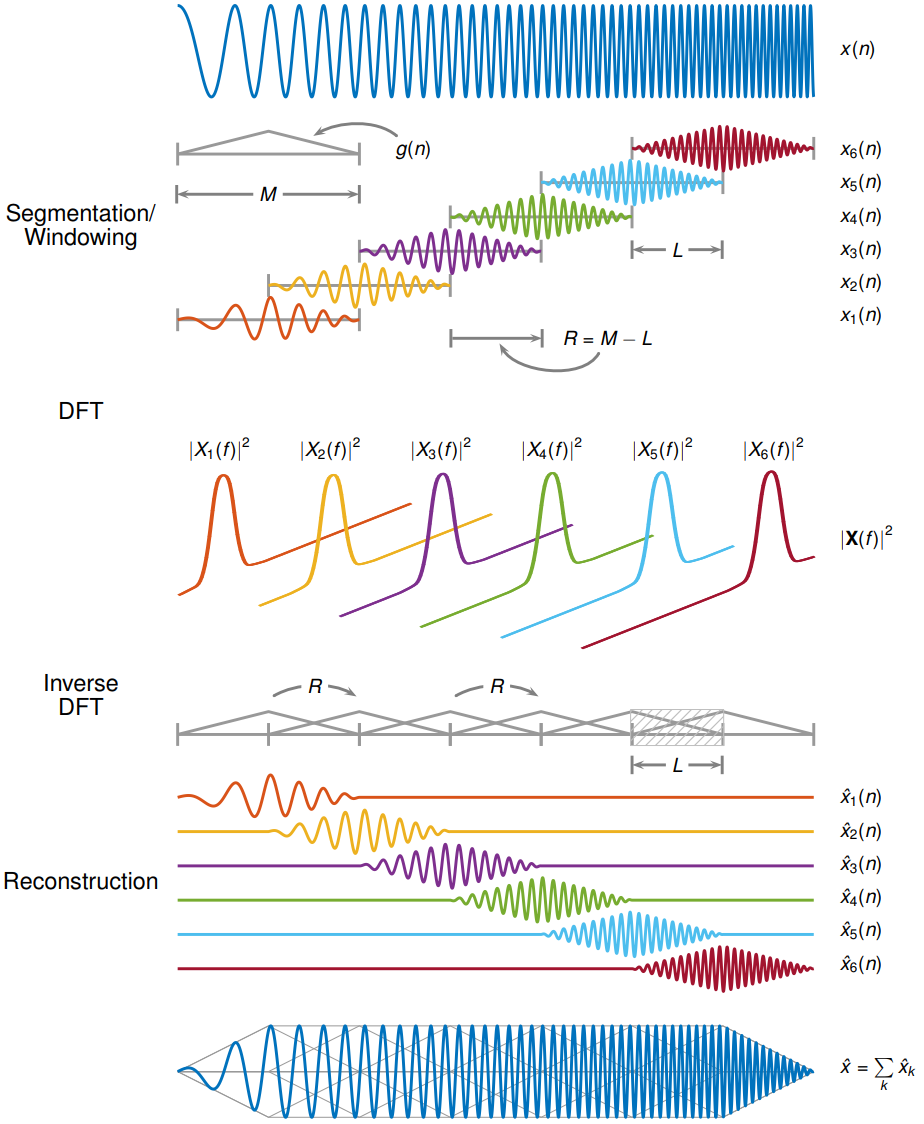
\includegraphics[height=8cm]{../images/iscola0111.png}
	\end{figure}
\end{frame}

\begin{frame}
	\frametitle{STFT, ISTFT}
	\begin{figure}
	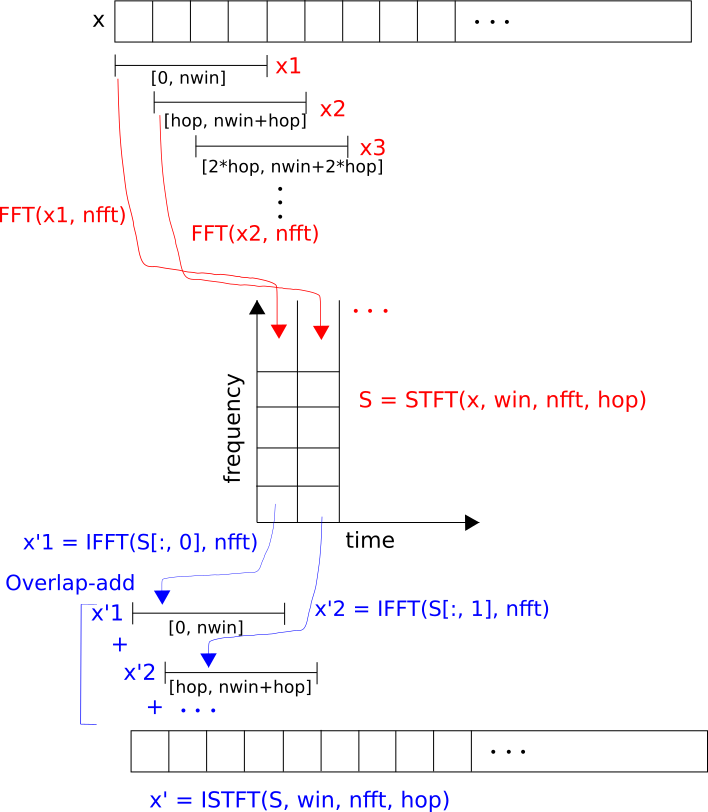
\includegraphics[height=8cm]{../images/stft_diagram.png}
	\end{figure}
\end{frame}

\begin{frame}
	\frametitle{``Round-trip'' through STFT}
	\begin{figure}
	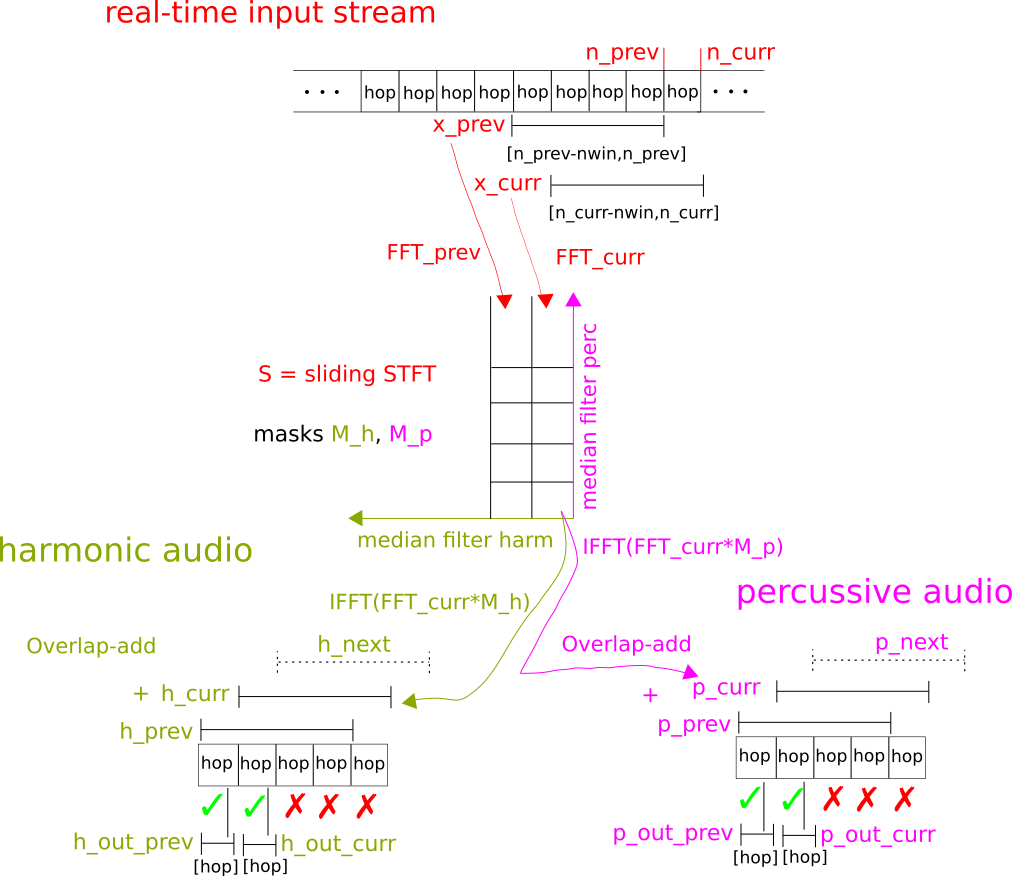
\includegraphics[height=8cm]{../images/rt_hpss_diagram.png}
	\end{figure}
\end{frame}

\begin{frame}
	\frametitle{Real-time HPSS}
	Input buffer \textit{x[1024]}, output buffers \textit{h[1024]}, \textit{p[1024]}, overlap = 512
	\begin{enumerate}
		\item Receive a chunk of 512 samples, \textit{x\_current}, from input stream
		\item Append to right of buffer \textit{x}: \textit{x = x[512:1024] + x\_current}
		\item Calculate FFT of \textit{x} and append to sliding STFT matrix
		\item Calculate harmonic, percussive masks with median filtering
		\item Apply IFFT to masked FFT to get \textit{h\_current}, \textit{p\_current}
		\item Weighted overlap-add: \textit{h = h + h\_current}, \textit{p = p + p\_current}
		\item \textit{h[0:512]}, \textit{p[0:512]} represent the correct, final harmonic/percussive separation of \textit{x\_current}
		\item Shift h, p left: \textit{h = h[512:1024] + zeros(512)}, \textit{p = p[512:1024] + zeros(512)} for future weighted overlap-add
		\item Repeat
	\end{enumerate}
\end{frame}

\begin{frame}[fragile]
	\frametitle{Sliding STFT}
	How big should the sliding STFT be? Median filter lengths vary slightly in the 2010 and 2014 variants:
	\begin{enumerate}
		\item $l_{\text{harm}}$ = $l_{\text{perc}}$ = 17
		\item $l_{\text{harm}}$ = 200ms in samples $\approx$ 12, $l_{\text{perc}}$ = 500Hz in samples $\approx$ 12
	\end{enumerate}
	k-point movmedian (median filter) in MATLAB \footfullcite{movmedian} uses a window centered at the current pixel extending $\frac{k}{2}$ to the left and to the right. For harmonic/horizontal median filter, we only need a history of $\frac{17}{2}$ or $\frac{12}{2}$ STFT columns to median-filter the current FFT/STFT column:
	\begin{small}
	\begin{verbatim}
	    STFT = zeros(nfft, ceil(lHarm/2));  % preallocate sliding stft
	    STFT = STFT(:, 2:size(STFT, 2)); % remove oldest stft frame 
	    STFT(:, size(STFT, 2)+1) = FFT_current; % append latest FFT
	\end{verbatim}
	\end{small}
	For percussive/vertical median filter, the current FFT/STFT column contains all of the necessary points.
\end{frame}

\begin{frame}
	\frametitle{Sliding STFT causality}
	The horizontal/harmonic median filtering doesn't have future STFT frames available in the real-time algorithm, so harmonic separation quality will most likely suffer. Given this, prefer binary masking in real-time implementation for the better separation quality.
	\begin{figure}
	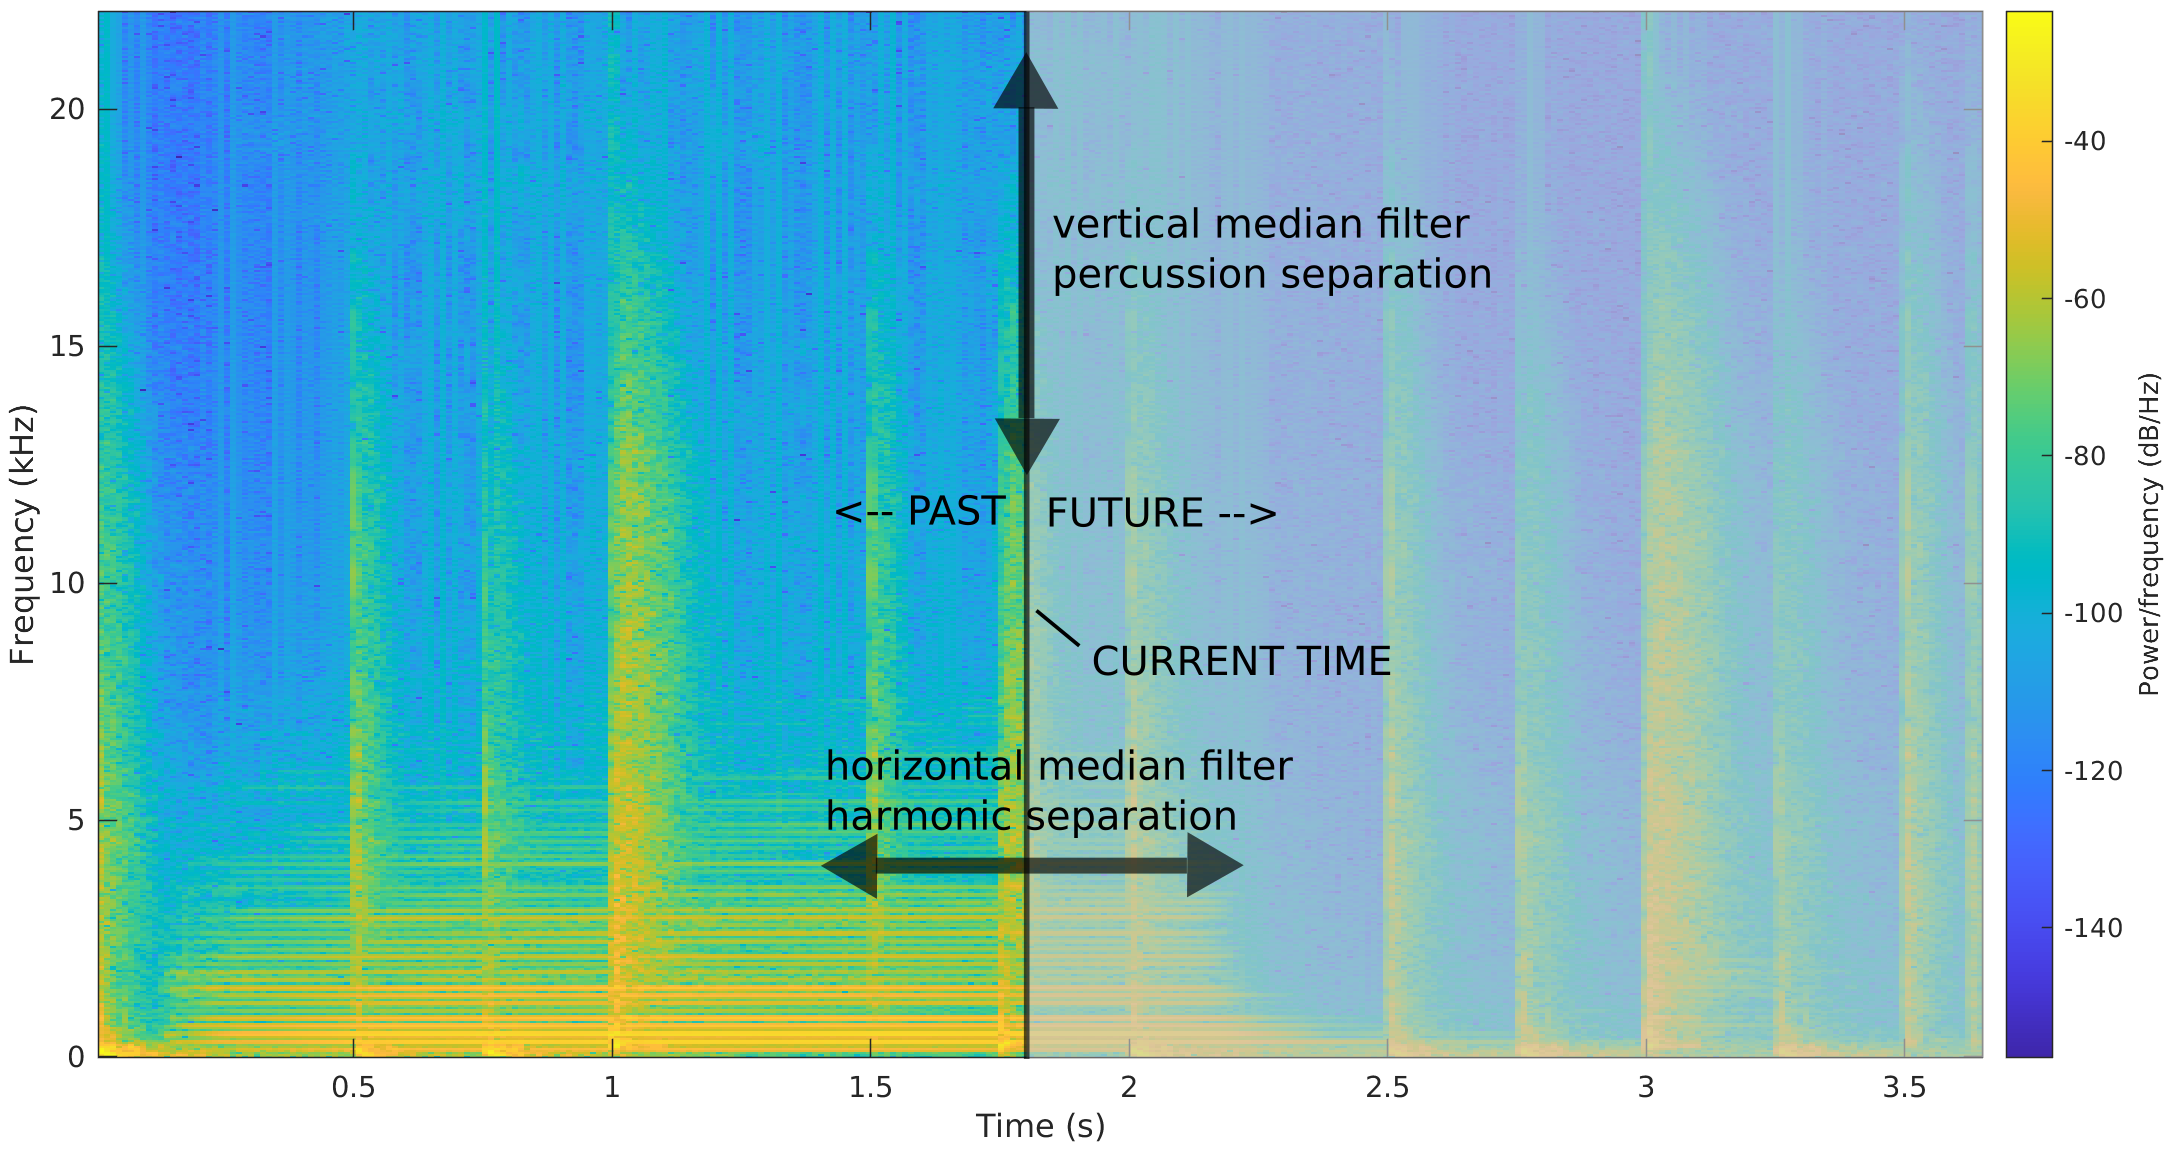
\includegraphics[height=5cm]{../images/hpss_causality.png}
		\caption{Causality problem of real-time HPSS}
	\end{figure}
\end{frame}

\begin{frame}
	\frametitle{Mixed sound}
	\href{run:../audio/mixed.wav}{Recall from earlier}\
	\begin{figure}
	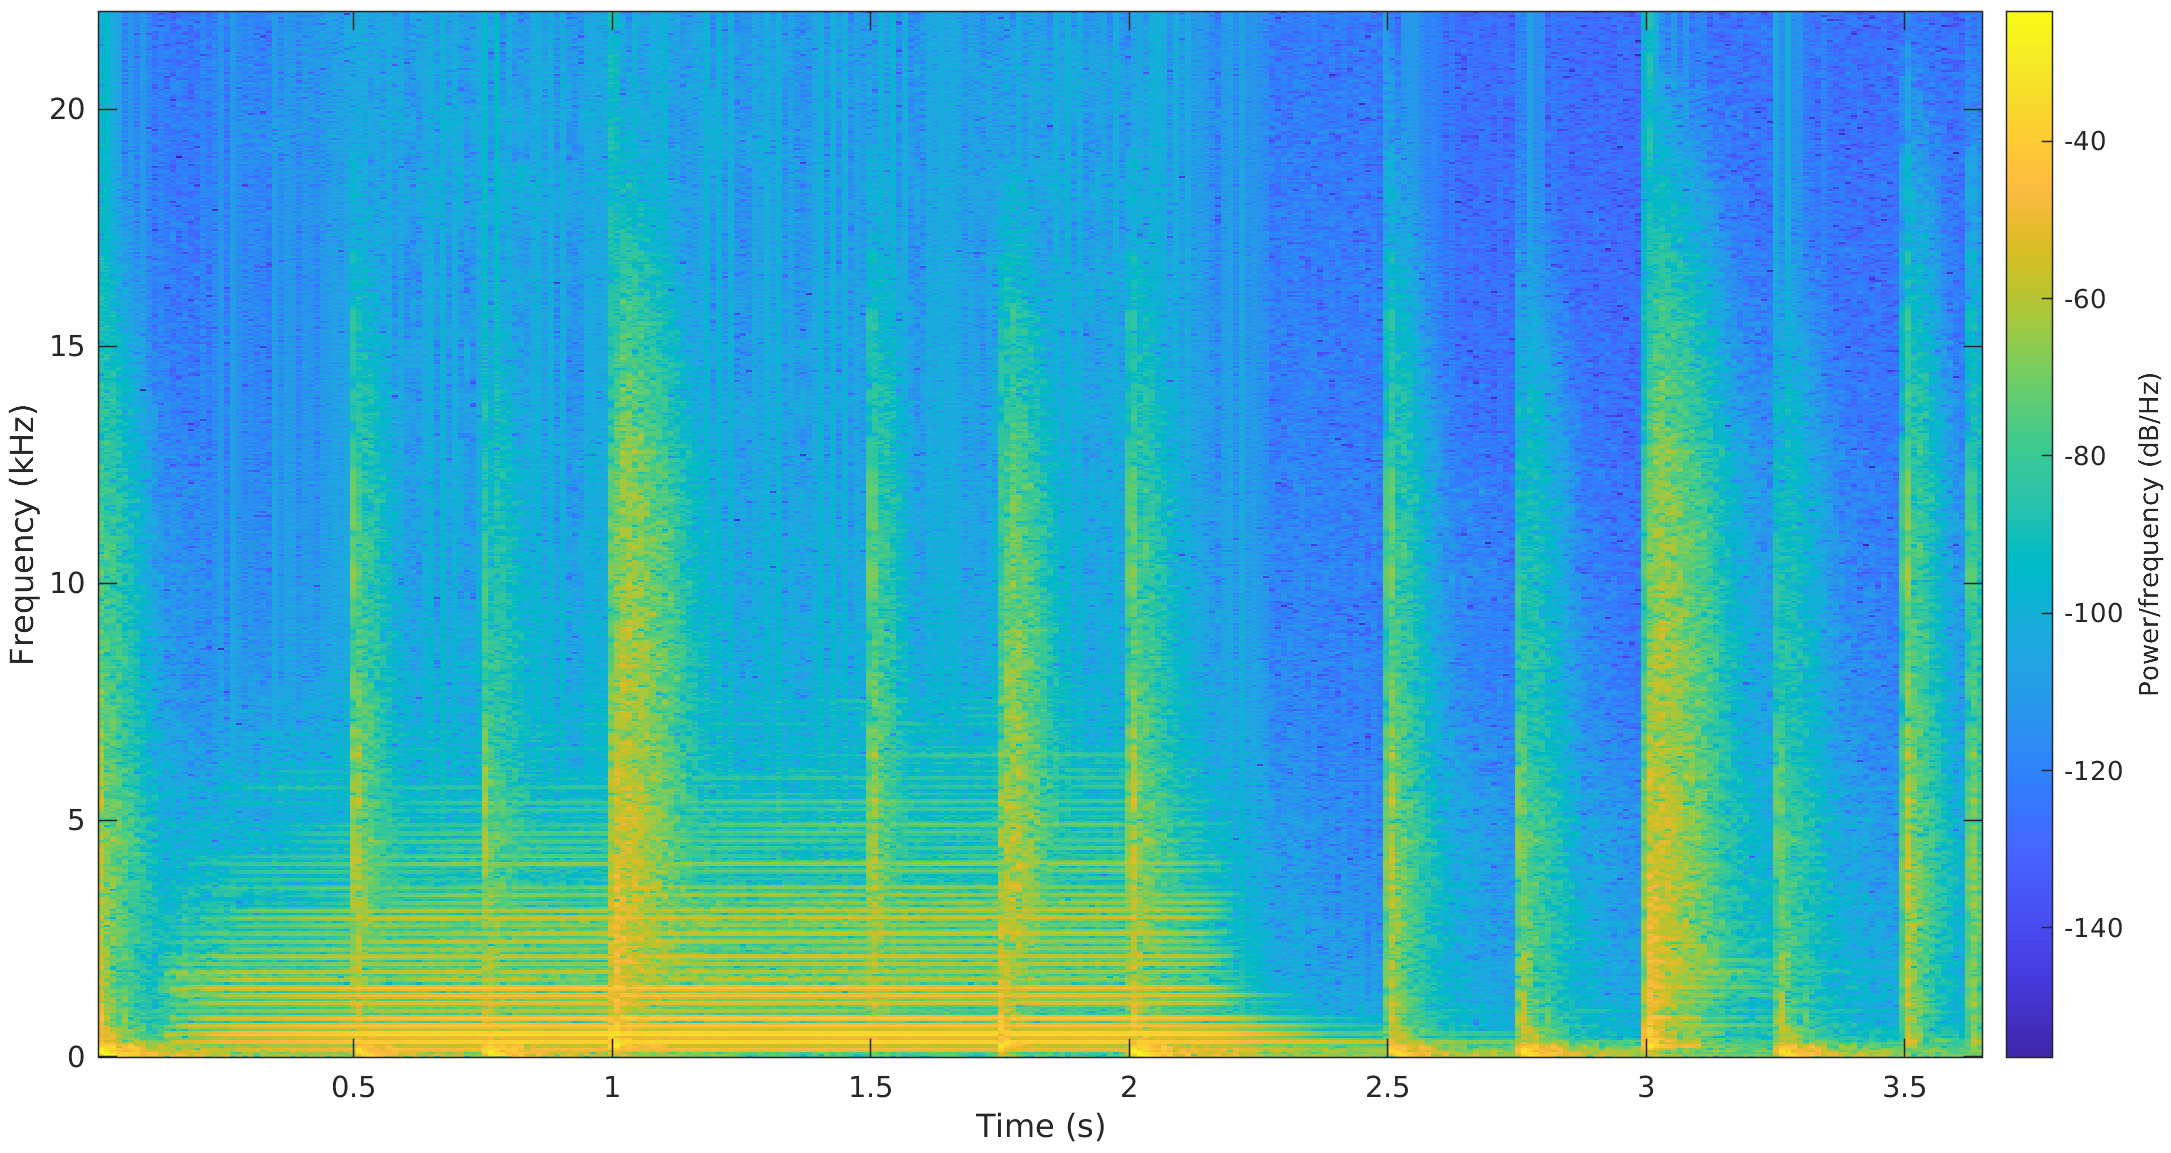
\includegraphics[height=5cm]{../images/mixedspecgram.png}
		\caption{Mixed spectrogram}
	\end{figure}
\end{frame}

\begin{frame}
	\frametitle{Real-time HPSS}
	\begin{figure}
	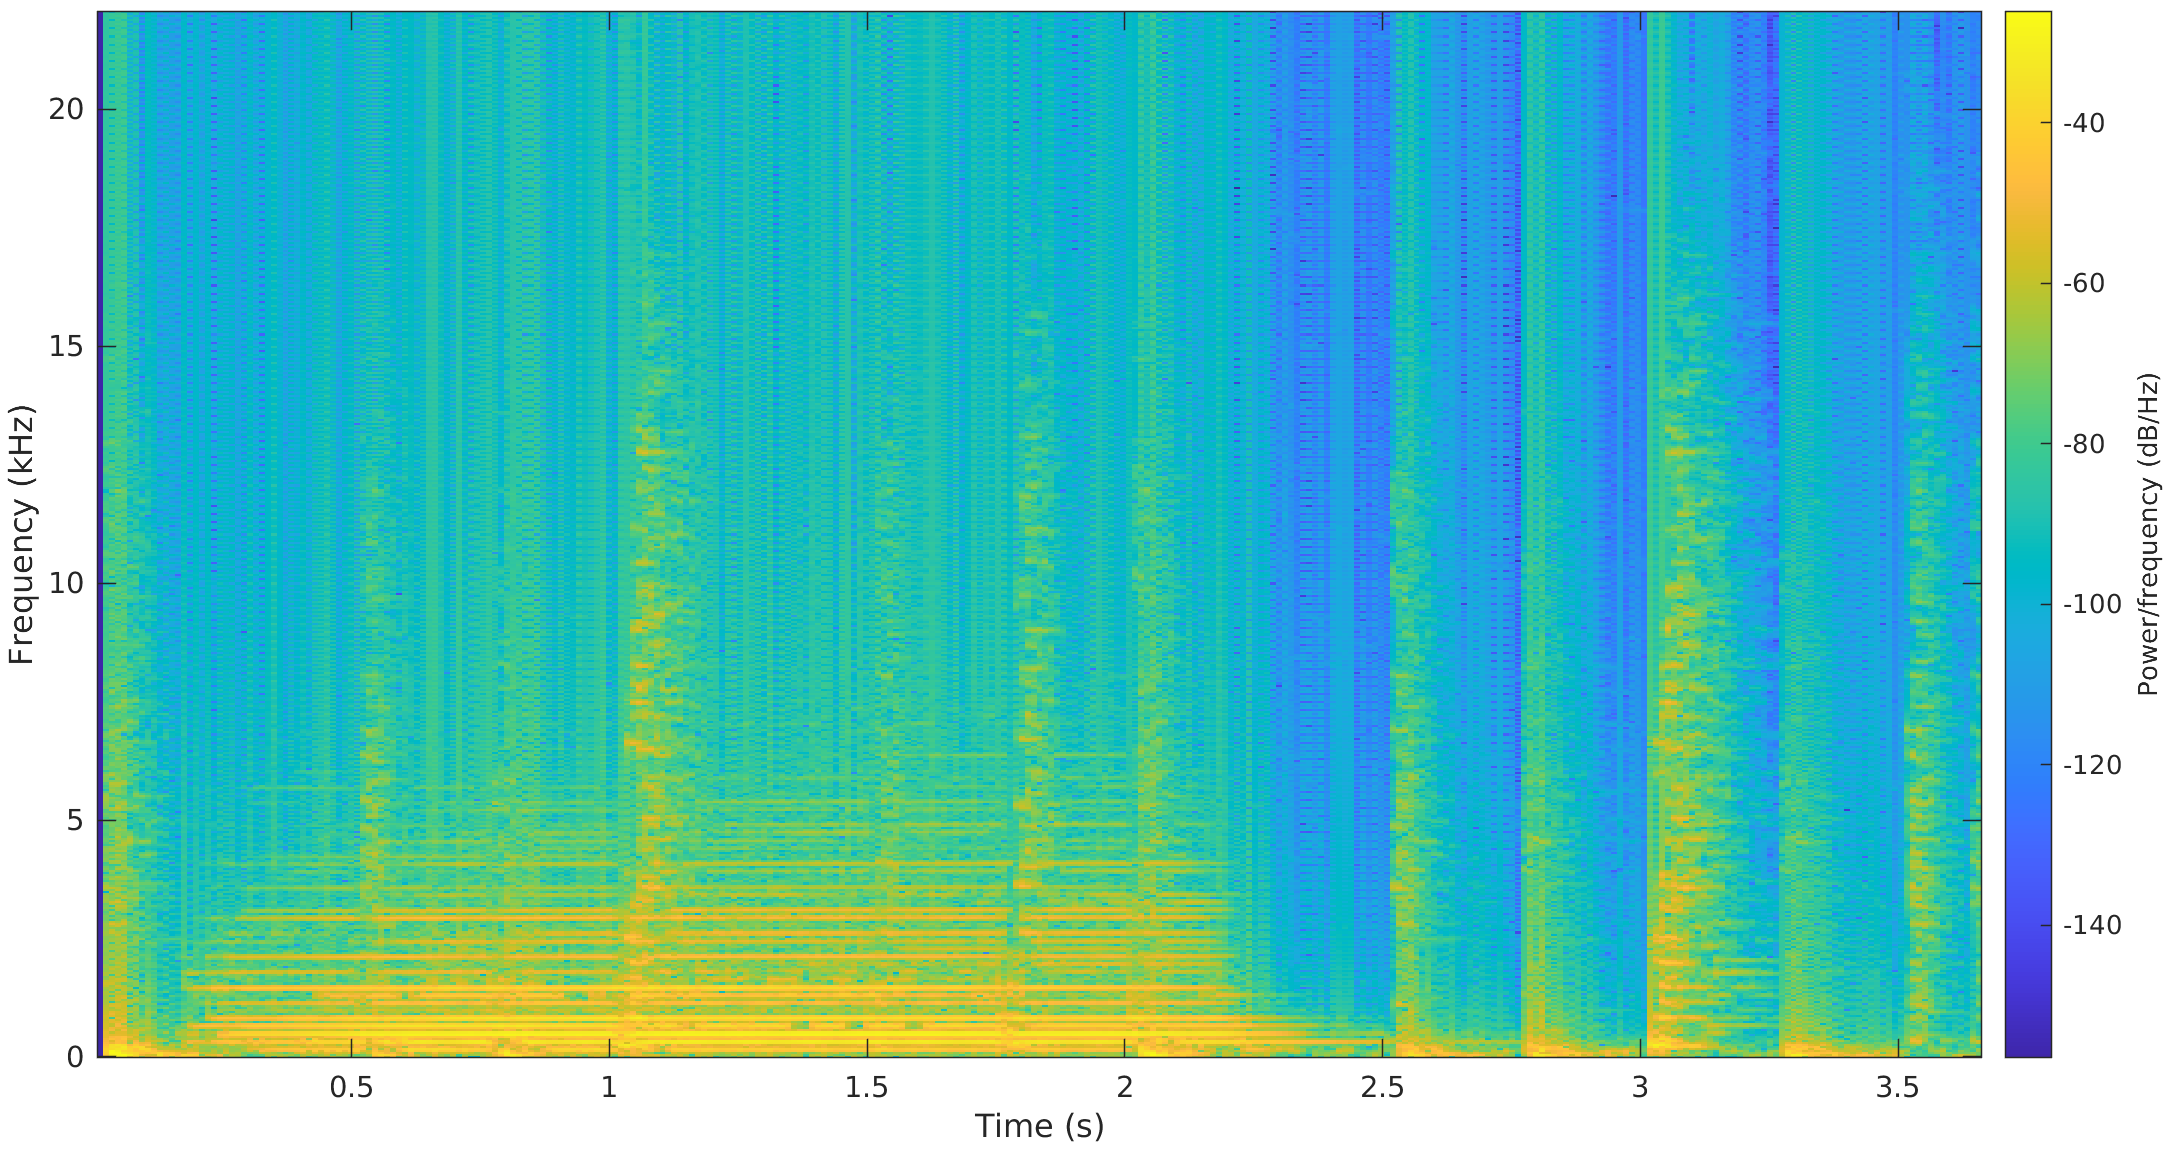
\includegraphics[height=5cm]{../images/harm_realtime.png}
		\caption{Separated harmonic spectrogram}
	\end{figure}
\end{frame}

\begin{frame}
	\frametitle{Real-time HPSS}
	\href{run:../audio/harm_rt.wav}{Click to listen}\\
	\begin{figure}
	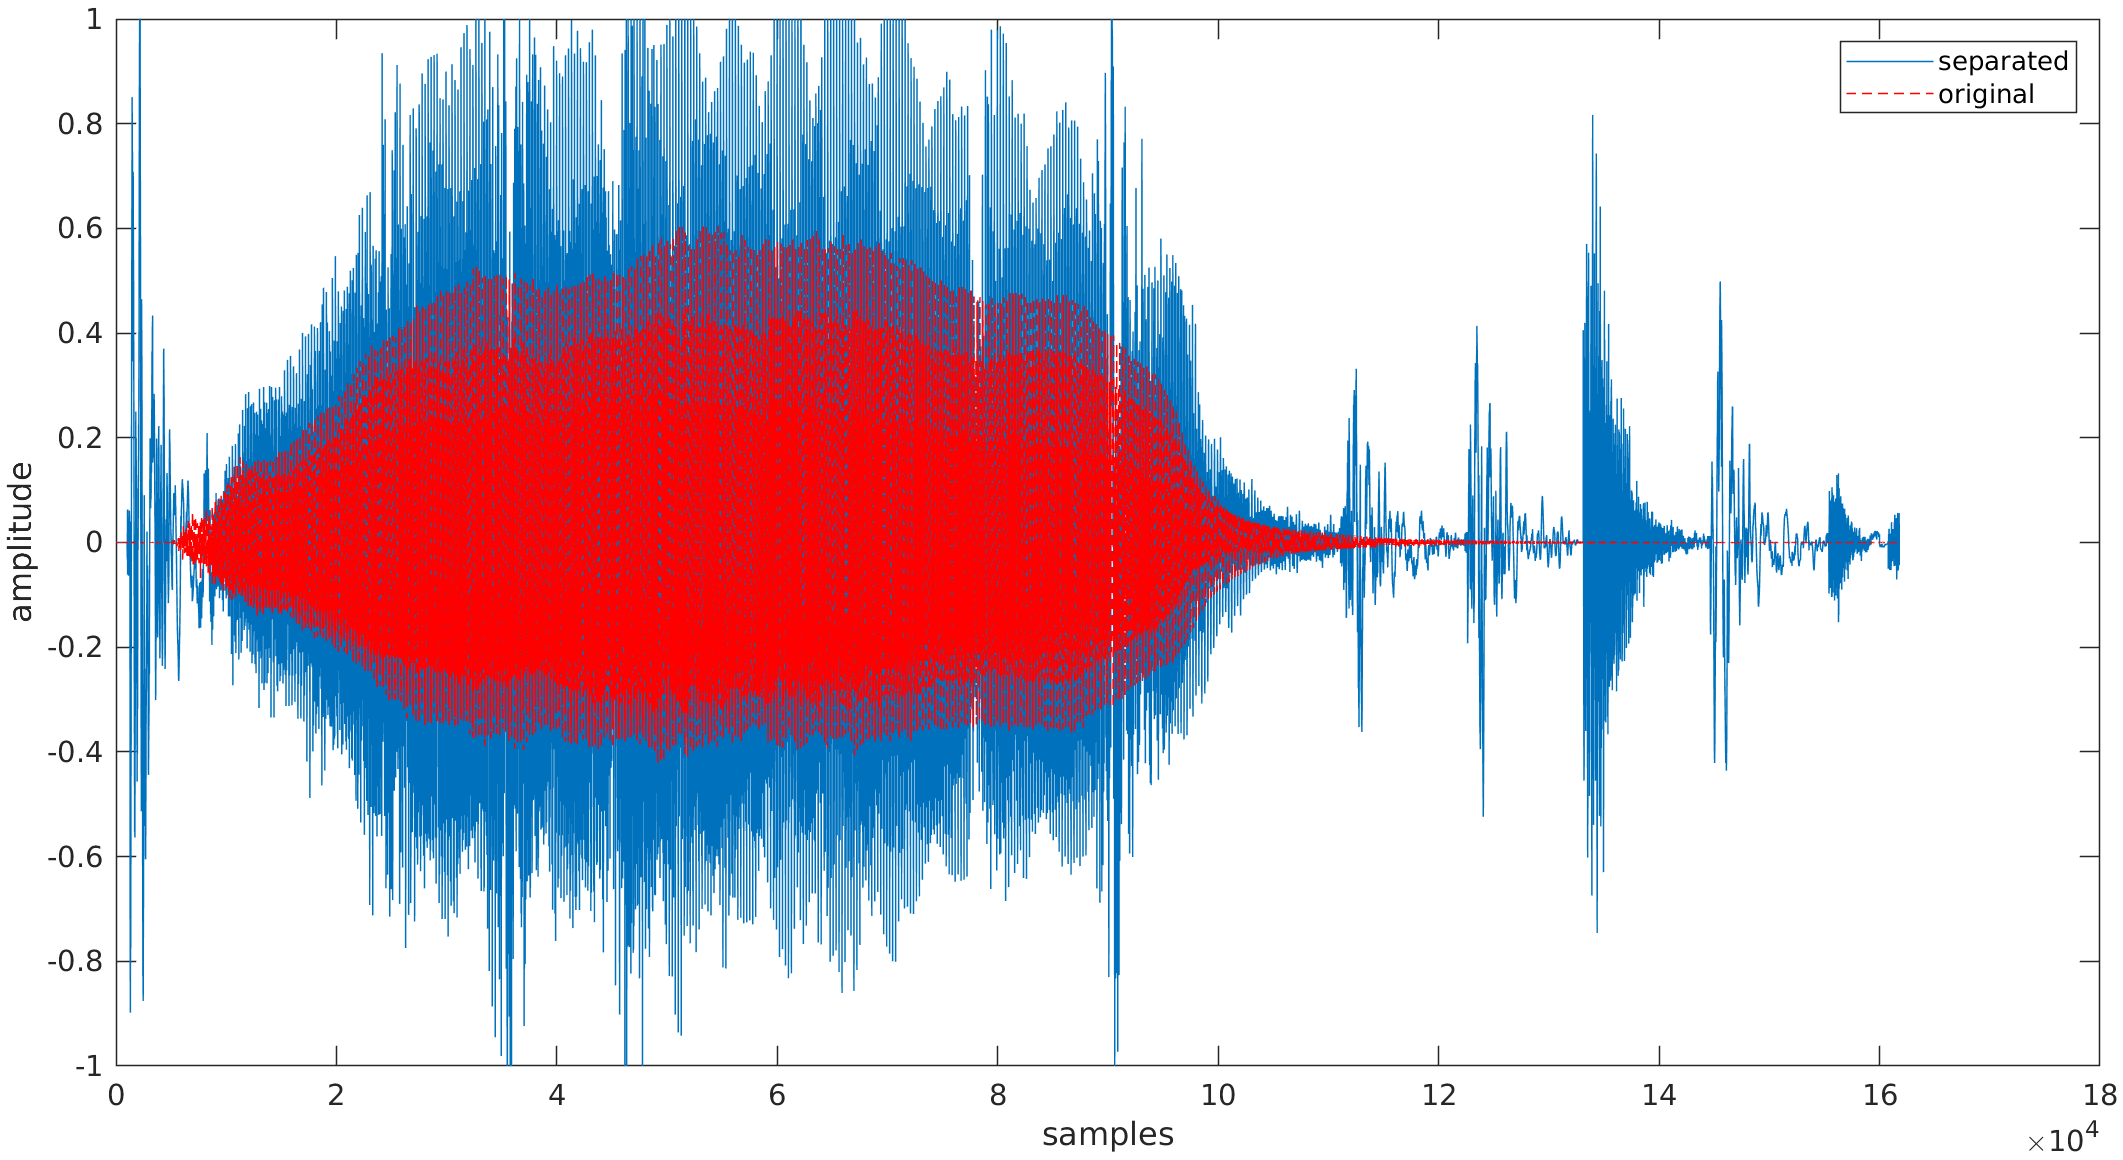
\includegraphics[height=5cm]{../images/harm_realtime_cmp.png}
		\caption{Harmonic waveform comparison}
	\end{figure}
\end{frame}

\begin{frame}
	\frametitle{Real-time HPSS}
	\begin{figure}
	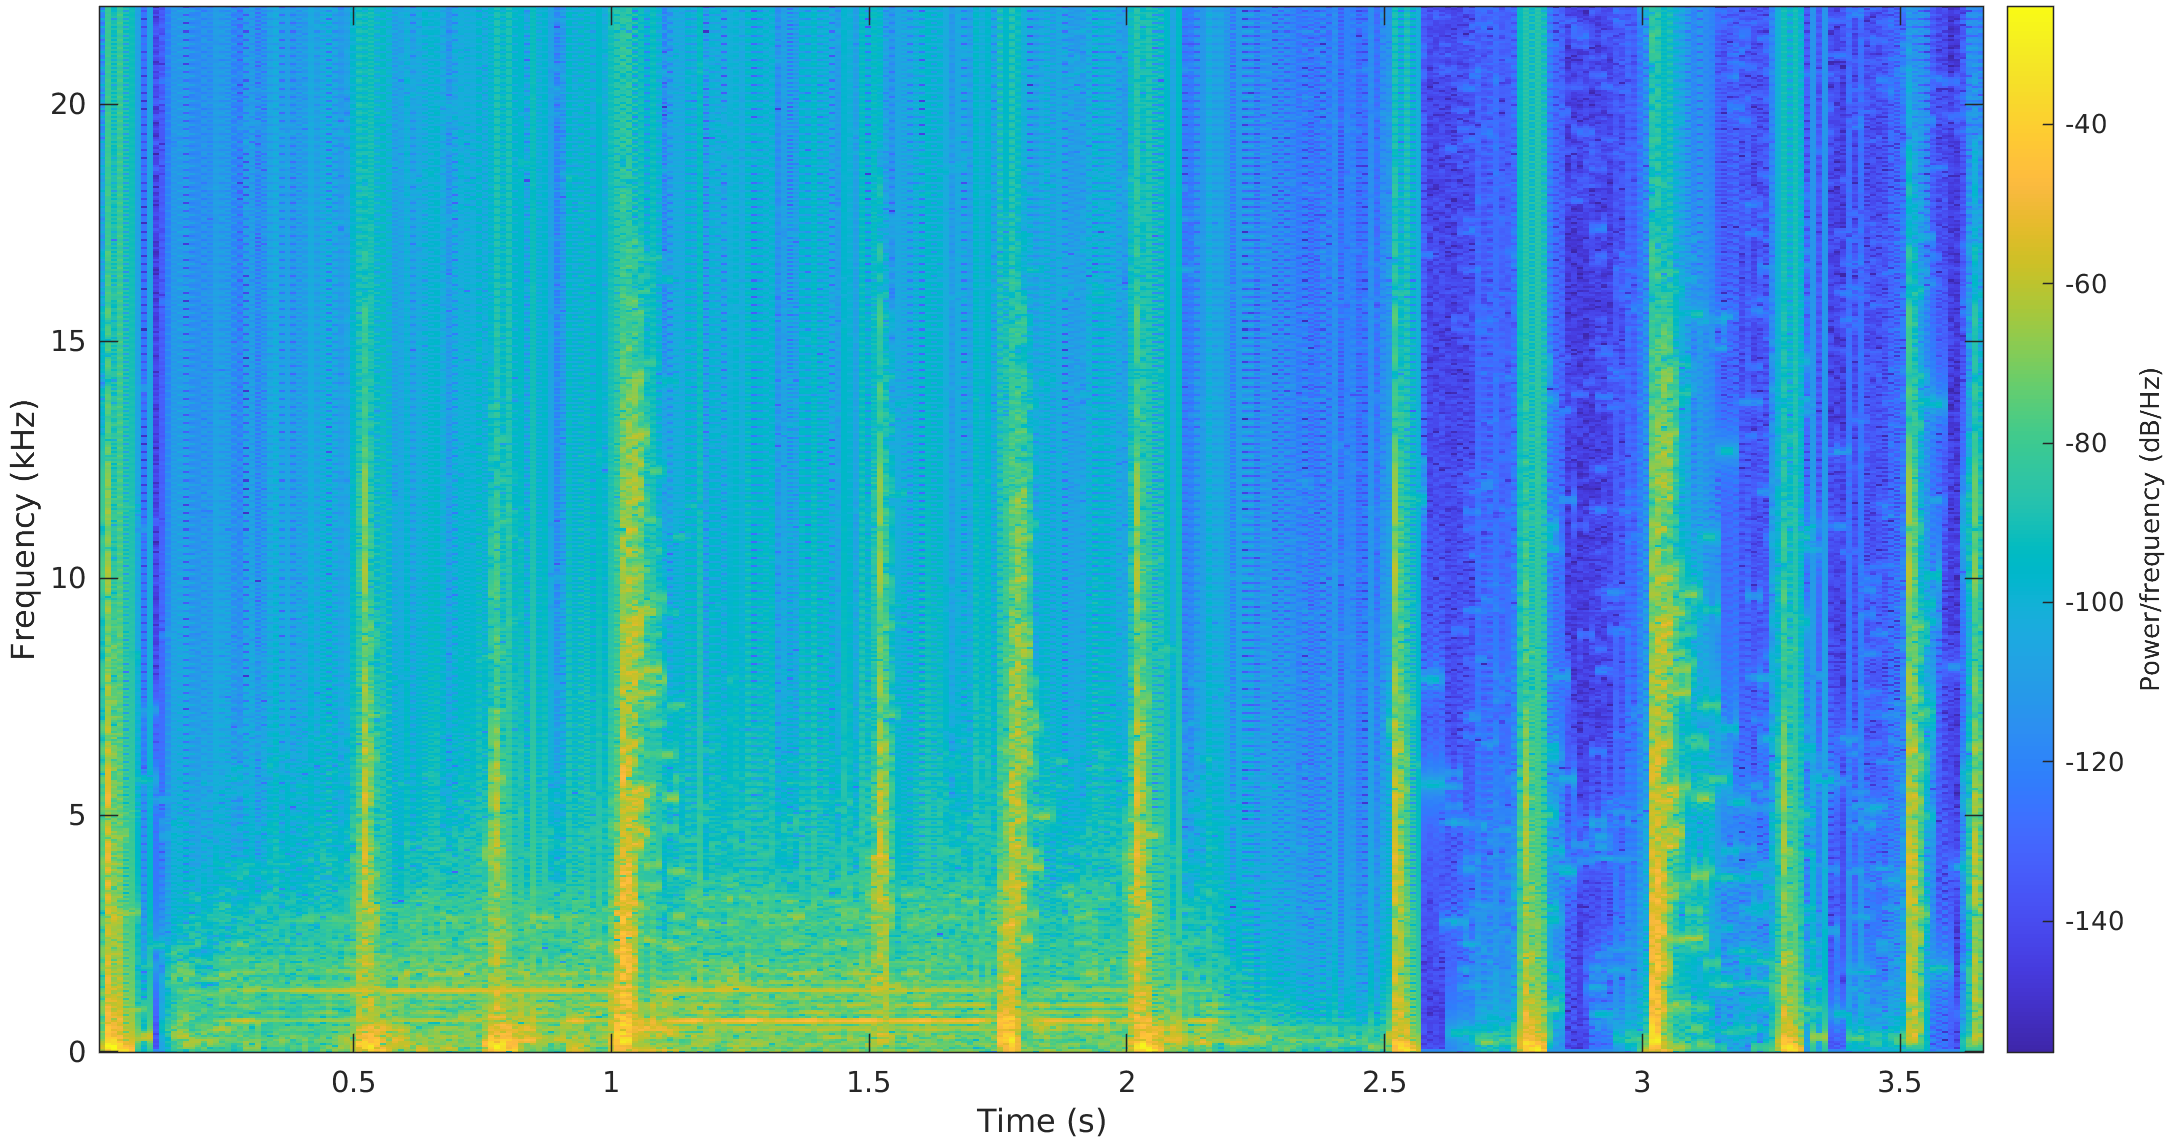
\includegraphics[height=5cm]{../images/perc_realtime.png}
		\caption{Separated percussive spectrogram}
	\end{figure}
\end{frame}

\begin{frame}
	\frametitle{Real-time HPSS}
	\href{run:../audio/perc_rt.wav}{Click to listen}\\
	\begin{figure}
	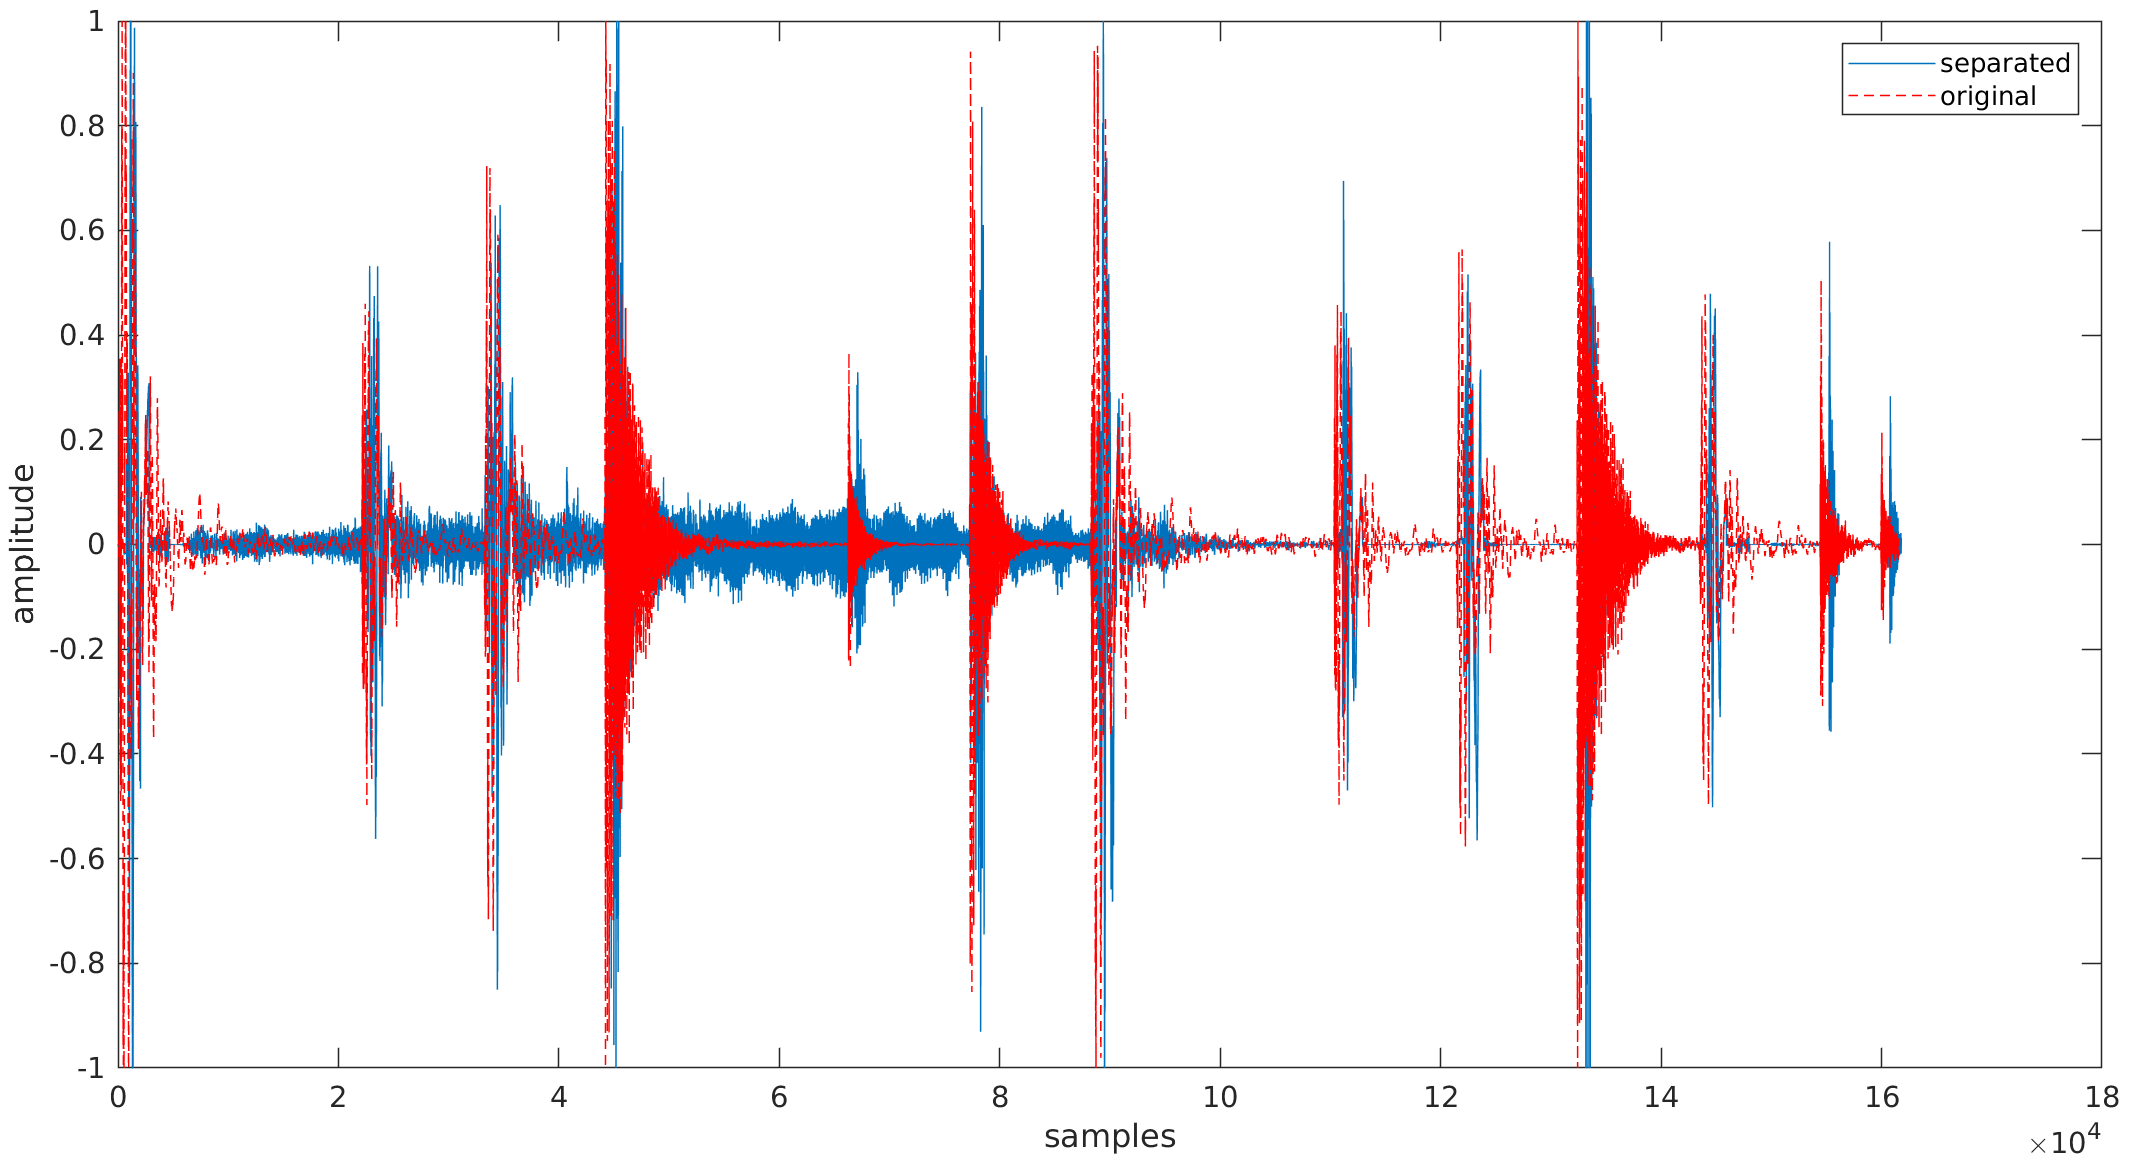
\includegraphics[height=5cm]{../images/perc_realtime_cmp.png}
		\caption{Percussive waveform comparison}
	\end{figure}
\end{frame}

\begin{frame}
	\frametitle{Real-time HPSS}
	\begin{figure}
	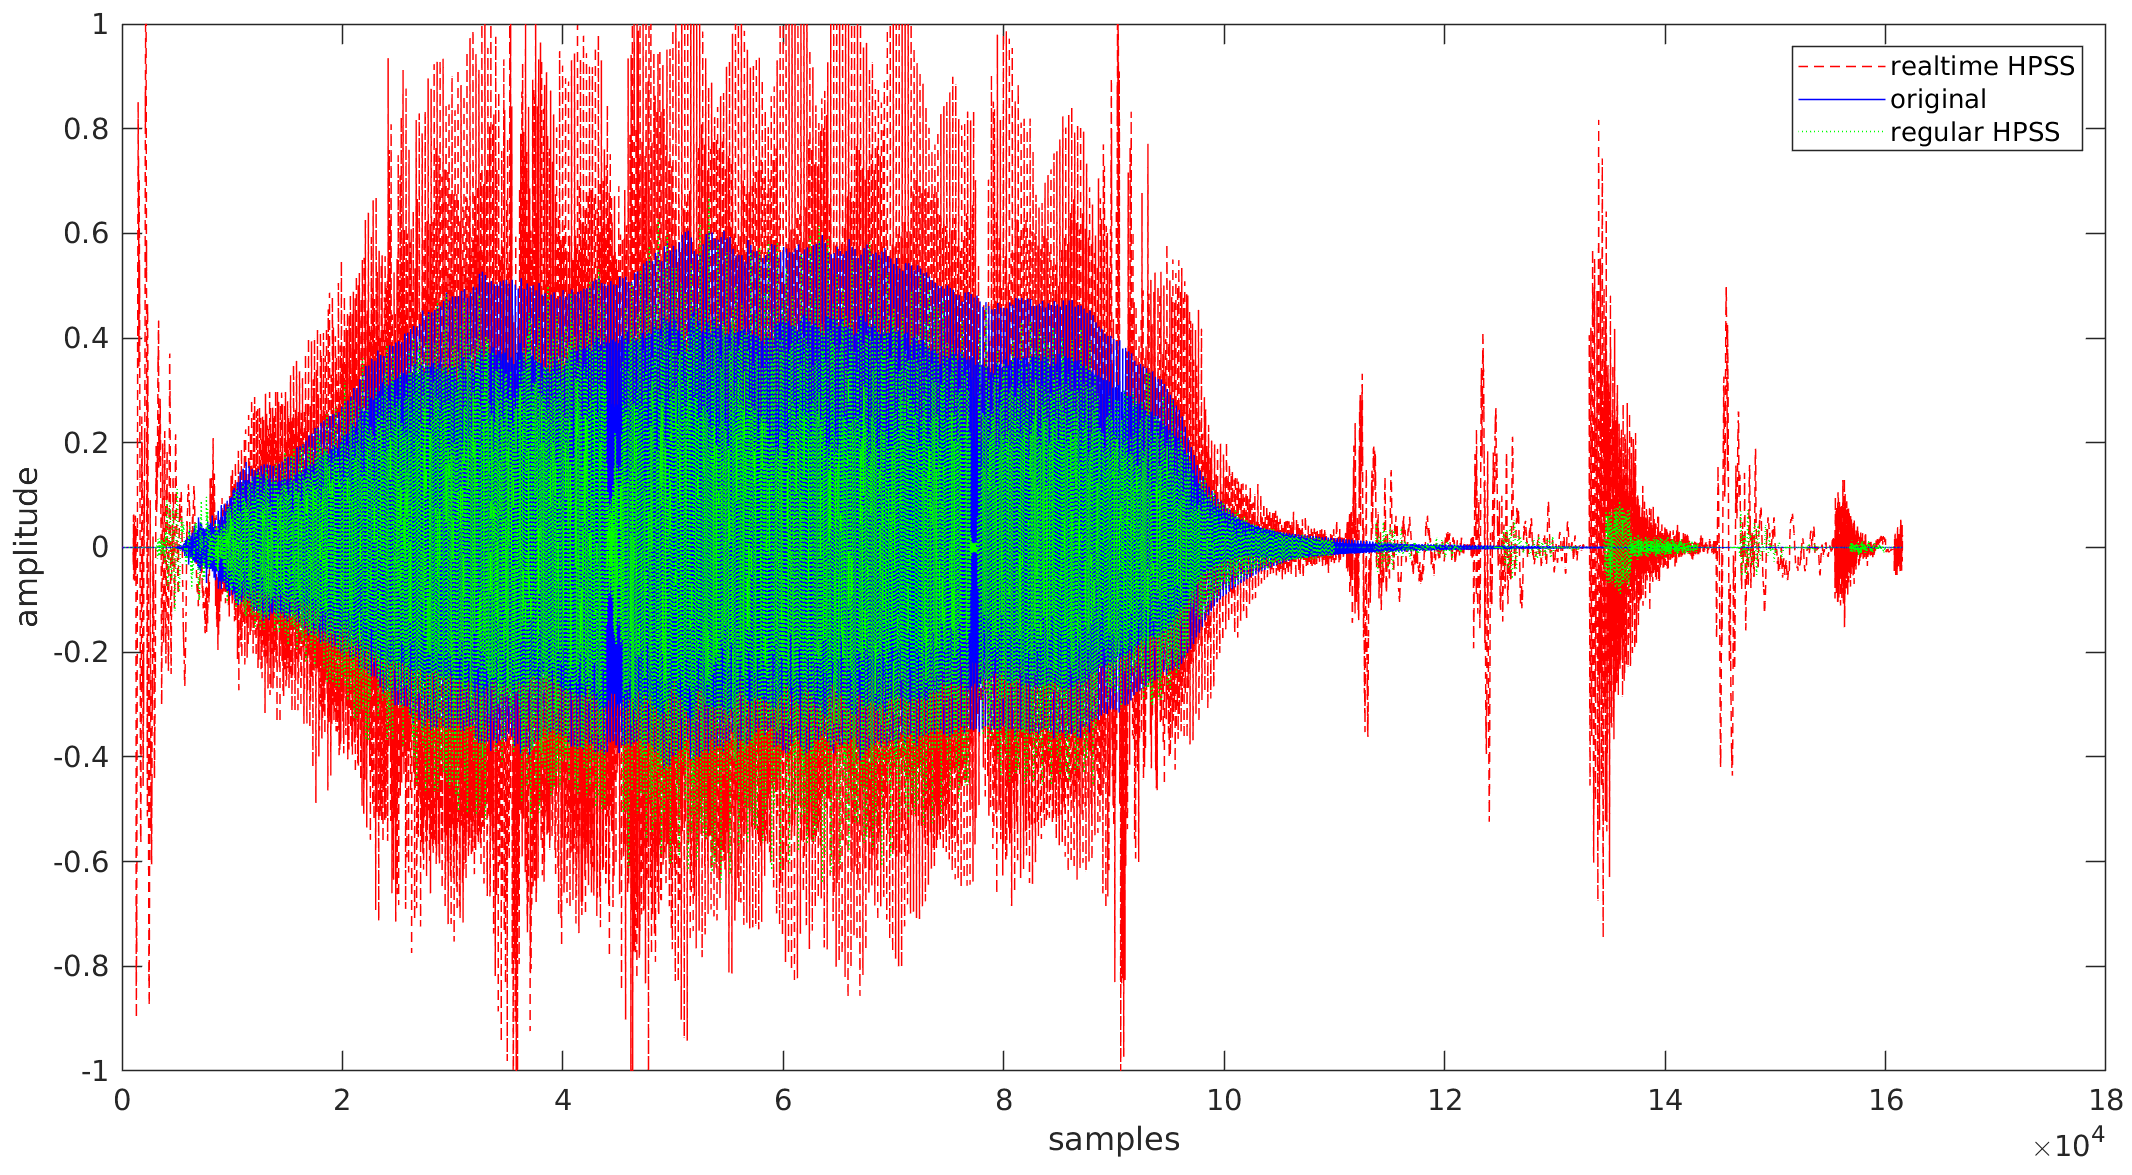
\includegraphics[height=5cm]{../images/harm_3way.png}
		\caption{Harmonic waveform comparison including offline HPSS}
	\end{figure}
\end{frame}

\begin{frame}
	\frametitle{Real-time HPSS}
	\begin{figure}
	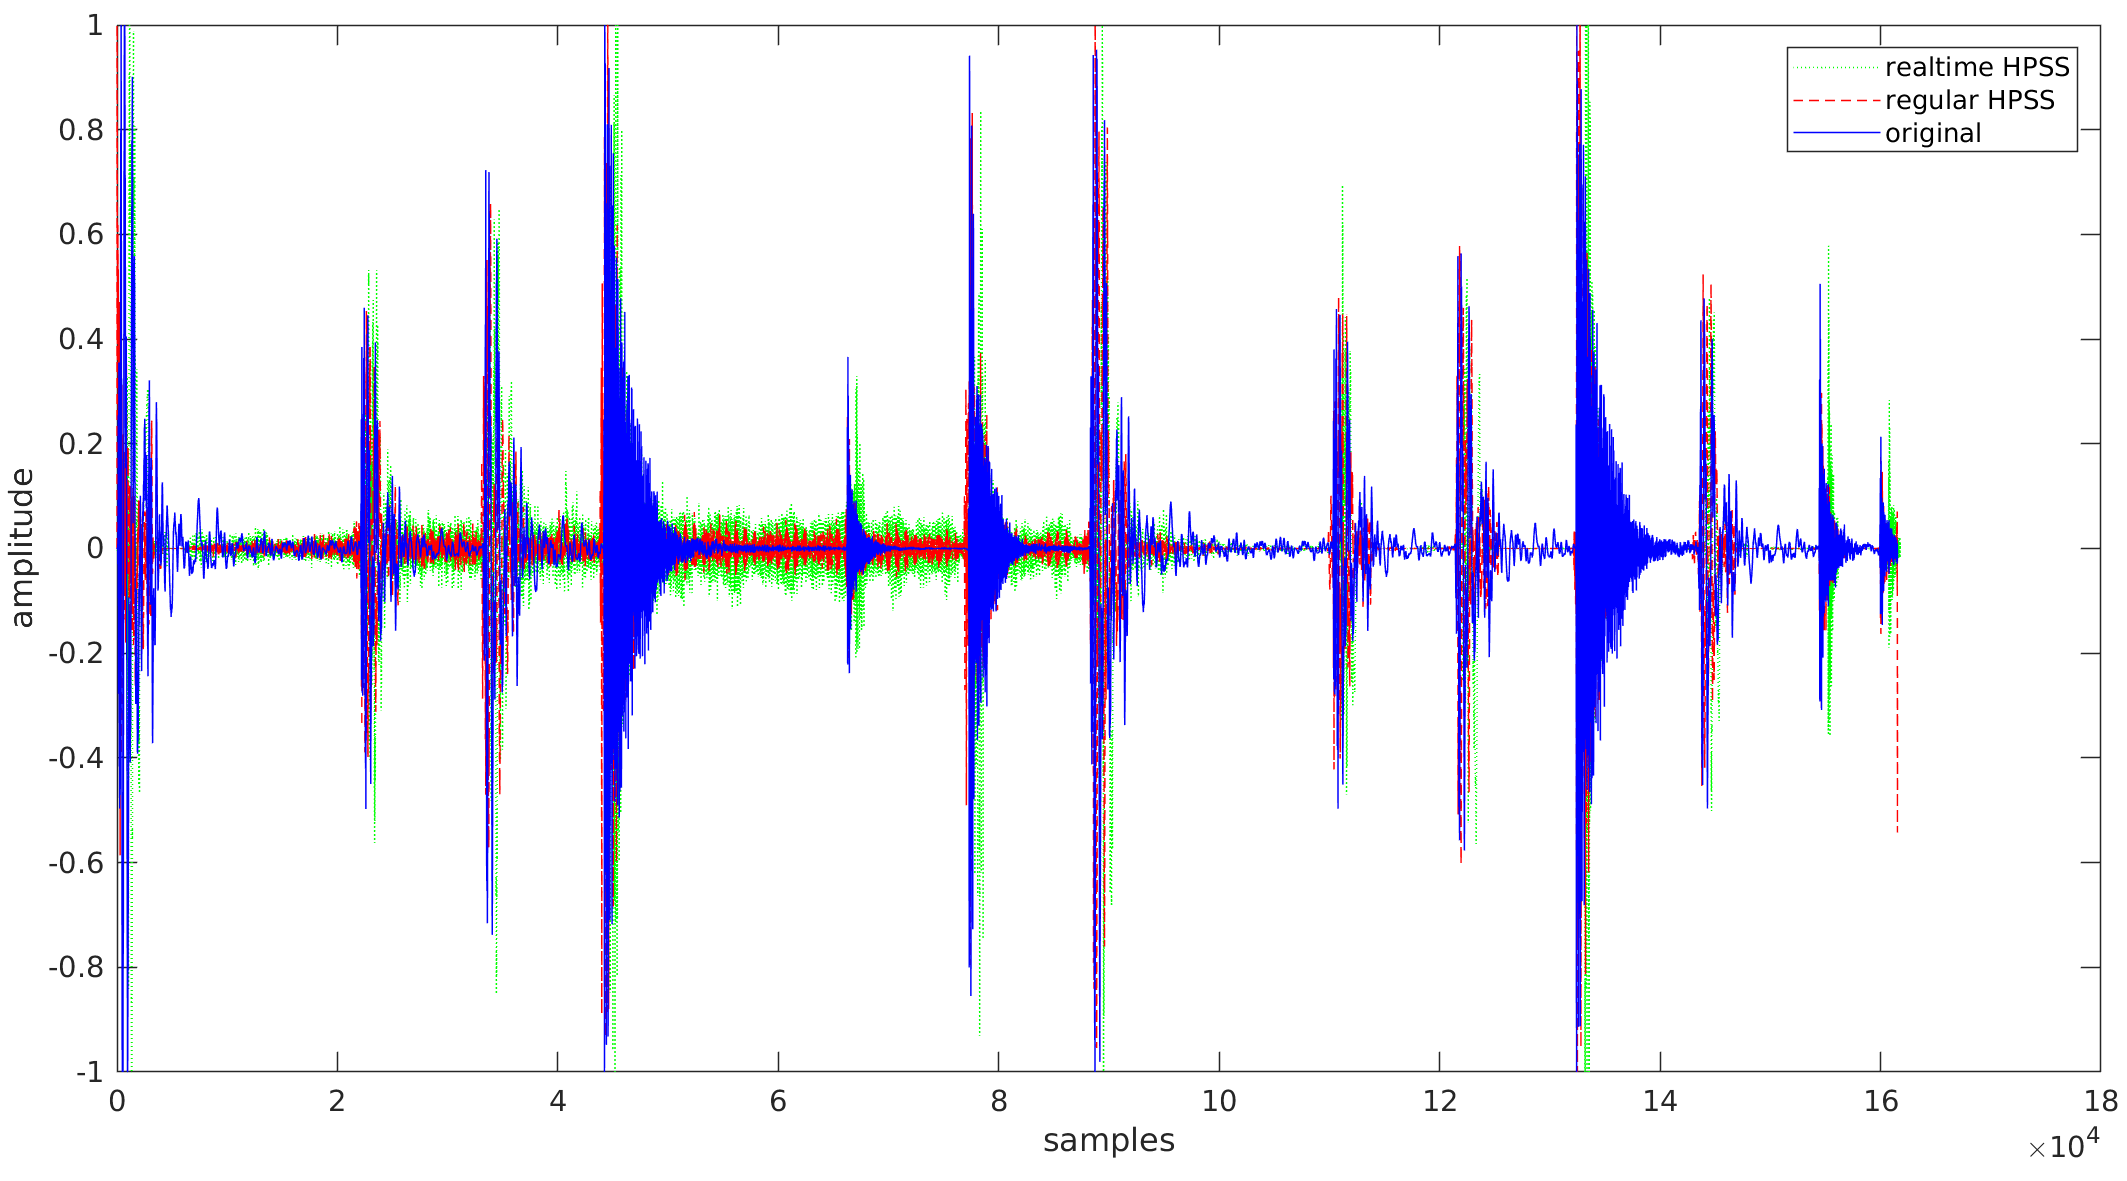
\includegraphics[height=5cm]{../images/perc_3way.png}
		\caption{Percussive waveform comparison including offline HPSS}
	\end{figure}
\end{frame}

\begin{frame}
	\frametitle{Complex example}
	\begin{figure}
	
\includegraphics[width=10cm]{../images/mestis_el_mestizo.jpg}
	\end{figure}
	\href{run:../audio/mestis_el_mestizo_shorter.wav}{original}, 
	\href{run:../audio/mestis_harm_offline_shorter.wav}{offline harmonic},
	\href{run:../audio/mestis_harm_rt_shorter.wav}{rt harmonic},
	\href{run:../audio/mestis_perc_offline_shorter.wav}{offline percussive},
	\href{run:../audio/mestis_perc_rt_shorter.wav}{rt percussive}
\end{frame}

\begin{frame}
	\frametitle{Conclusions}
	\begin{enumerate}
		\item Learned what HPSS is and why it matters
		\item Described, implemented, and showed results of median-filtering HPSS (2010, 2014)
		\item Adapted HPSS to real-time with STFT--ISTFT ``roundtrip''
		\item Showed that real-time HPSS produces acceptable percussive separation
		\item Future ideas: apply heuristics to improve real-time harmonic separation
	\end{enumerate}
\end{frame}

\end{document}
